% This must be in the first 5 lines to tell arXiv to use pdfLaTeX, which is strongly recommended.
\pdfoutput=1
% In particular, the hyperref package requires pdfLaTeX in order to break URLs across lines.

\documentclass[11pt]{article}

% Change "review" to "final" to generate the final (sometimes called camera-ready) version.
% Change to "preprint" to generate a non-anonymous version with page numbers.
\usepackage[preprint]{acl}

% Standard package includes
\usepackage{times}
\usepackage{latexsym}
\usepackage{tikz}


% For proper rendering and hyphenation of words containing Latin characters (including in bib files)
\usepackage[T1]{fontenc}

% This assumes your files are encoded as UTF8
\usepackage[utf8]{inputenc}

% This is not strictly necessary, and may be commented out,
% but it will improve the layout of the manuscript,
% and will typically save some space.
\usepackage{microtype}

% This is also not strictly necessary, and may be commented out.
% However, it will improve the aesthetics of text in
% the typewriter font.
\usepackage{inconsolata}

%Including images in your LaTeX document requires adding
%additional package(s)
\usepackage{graphicx}

% Added packages by authors, will comment them out if necessary.
\usepackage{xcolor}
\usepackage{xcolor,colortbl}
\definecolor{hidden-draw}{RGB}{0,0,0}

\usepackage{tikz}
\usepackage[edges]{forest}


\usetikzlibrary{trees,positioning,shapes,shadows,arrows.meta}

\renewcommand{\baselinestretch}{0.96}


\title{PlanGenLLMs: A Modern Survey of LLM Planning Capabilities}

\author{Hui Wei,$^\dagger$ Zihao Zhang,$^\ddagger$ Shenghua He,$^\S$ Tian Xia,$^\S$\\ 
\textbf{Shijia Pan,$^\dagger$ Fei Liu$^\ddagger$}\\[0.5em]
$^\dagger$University of California, Merced \, 
$^\ddagger$Emory University\, 
$^\S$PAII Inc.\\
\texttt{\{huiwei2, span24\}@ucmerced.edu}\\
\texttt{\{zihao.zhang, fei.liu\}@emory.edu}
\texttt{\quad \{shenghh2015, TianXia0209\}@gmail.com} \\ 
}


\begin{document}
\maketitle
%%%% ABSTRACT %%%%


\begin{abstract}

We study a data marketplace where a broker facilitates transactions between buyers and contributors. Buyers seek to estimate the mean \(\mu\) of an unknown normal distribution \(\mathcal{N}(\mu, \sigma^2)\), but have varying valuations based on their estimation error. Contributors, each with different data collection costs, gather samples from this distribution and report them (not necessarily truthfully) to the broker. The broker then sells subsets of the combined dataset to buyers at varying prices and redistributes the revenue to contributors. 
%
We formalize this as a mechanism design problem aimed at maximizing profit (total revenue minus data costs) while satisfying key market constraints: individual rationality (buyers and contributors benefit from participation), envy-freeness (no buyer prefers another’s allocation), budget balance (total payments match revenue), and incentive-compatibility (contributors are incentivized to collect a sufficient amount of data report it truthfully).  

We design a mechanism which satisfies these requirements.
We first establish a connection between envy-free data pricing and ordered-item pricing (OIP) for unit-demand buyers and leverage OIP algorithms to determine the optimal data allocation and expected prices for buyers. The actual prices paid by buyers are centered around these expected prices, but also vary based on discrepancies in contributors' reported data. This variation is then passed on to the contributors via their payments.
This scheme results in a Nash equilibrium (NE) where only the two lowest-cost contributors collect all the data and report it truthfully.
% We also show that this NE is individually rational for buyers, satisfies budget balance, and maximi
Including this variation in the prices also helps us achieve individual rationality for buyers, as buyers will pay less if there are significant discrepancies in contributors' datasets.


To complement these findings, we prove a nearly matching upper bound on the maximum possible profit achievable in any NE of any mechanism, thus proving that our mechanism is essentially unimprovable.
We also show that no nontrivial dominant-strategy incentive-compatible mechanism exists in this problem. 


\end{abstract}

%%%% INTRODUCTION %%%%
\section{Introduction}

With the ubiquity of AI, \emph{data} has become a critical economic resource
driving operations and innovation across many domains.
However, not everyone has the means to
collect data on their own
 and thus must rely on \emph{data marketplaces} to acquire the data they
need. For instance, materials data platforms (e.g.~\citep{citrine}) aggregate datasets
from proprietary sources; smaller organizations and academic researchers, who do not have
access to extensive experimental infrastructure, can purchase this
data to advance their research.
% \ac{redundant sentence ``materials''?}
In recent years, data marketplaces have emerged across various domains,
including 
% materials science~\cite{citrine},
advertising~\cite{googleads,databrickssharing},
computer systems~\cite{azuredatashare,awshub},
insurance~\cite{datarade},
freight~\cite{freightdat},
logistics~\cite{bloombergeap}, 
and others~\citep{awsdataexchange,ibmdatafabric,snowflake}. 
As shown in~\fig~\ref{fig:datamarketplace},
these platforms act as intermediaries,
facilitating data purchases between buyers and contributors.
%\kkcomment{Insert a figure here illustrating a marketplace.}


% \begin{figure}[h!] \label{fig:datamarketplace}
%     \centering
%     \includegraphics[width=0.4\textwidth]{figure1.png} % Replace with the path to your image
%     \caption{Data Marketplace}
%     \label{fig:your_label} 
% \end{figure}

\begin{figure*}[b]
\vspace{-0.06in}
\centering
\includegraphics[width=0.99\linewidth]{figs/data_marketplace_v2}
\vspace{-0.12in}
\caption{\small%
An illustration of a data marketplace.
(1) Data contributors collect and submit their data.
(2) A \emph{broker} operating the marketplace evaluates
 the quality of their submissions and prices the data.
(3) The broker sells subsets of this dataset to the buyers.
(4) The revenue is redistributed back to the contributors.
\label{fig:datamarketplace}
}
\end{figure*}



\parahead{Untruthful data reporting} 
In data marketplaces, buyers seek high-quality data for their learning tasks, while contributors aim to maximize their profits. Aligning these incentives of buyers and contributors presents a significant challenge.
Strategic contributors seek to minimize their data collection costs, while maximizing their compensation from buyers.
Buyers, on the other hand, pay for data but may question its reliability, particularly when contributors act in self-interest.
These dynamics raise two critical and closely connected questions which we wish to address in this work:
First, are buyers receiving reliable data commensurate with the price they pay?
%Are buyers being treated fairly, relative to other buyers?
%Are contributors being adequately compensated for their efforts?
Second, are contributors incentivized to provide reliable data rather than prioritizing personal profit, say, for instance, by submitting fabricated (fake) data instead of genuinely collecting it?



%Second para: Something lacking in current literature: focus on the incentives of buyers and contributors jointly.

%\parahead{Motivating challenges}
%However, designing mechanisms that maximize profit, provide value to buyers, incentivize truthful data reporting from contributors, and 

% \parahead{Incentives of Buyers and Contributors} 
% In data marketplaces buyers seek high-quality data for their learning tasks, while contributors aim to maximize their profits. Aligning these incentives of buyers and contributors presents a significant challenge.
% Strategic contributors seek to minimize their data collection costs, while maximizing their compensation from buyers.
% Buyers, on the other hand, pay for data but may question its reliability, particularly when contributors act in self-interest.
% These dynamics raise several critical questions:
% Are buyers receiving reliable data commensurate with the price they pay?
% Are buyers being treated fairly, relative to other buyers?
% Are contributors being adequately compensated for their efforts?
% Are contributors incentivized to provide reliable data rather than prioritizing personal profit, say, for instance, by submitting fabricated (fake) data instead of genuinely collecting it?





\parahead{Positioning}
Most prior work on data marketplaces sets prices for buyers and payments to contributors based on \emph{quantity of data}.
This overlooks the fact that buyers ultimately care about performance on a given learning task.
Quantity-based pricing fails when strategic contributors can report untruthfully.
For instance, naively paying contributors based on the size of the dataset they contribute, incentivizes them to report large fabricated (fake) datasets to inflate earnings.

Addressing this requires a \emph{joint} analysis of buyer and contributor incentives.
For instance, in the naive mechanism above, contributors may benefit from fabricating data, but if buyers lose trust in data quality, they may exit the market, reducing revenue and  eventually harming contributors.
To retain buyers, pricing must be adjusted to reflect data quality.
These adjustments should then be passed on to contributors to incentivize truthful (high quality) data submissions.
While there is prior work on incentivizing truthful data reporting, they do not consider broader market constraints, e.g. contributor payments must originate from buyers who derive value from the data they purchase.
%We discuss these distinctions further %in~\S\ref{sec:relatedwork}.

\parahead{Model}
We study these questions in a mean estimation problem. A finite set of data contributors $\contributors$, collect data from the same but unknown normal distribution $\Ncal(\mu,\sigma^2)$, with each contributor  incurring a different cost  per sample.
A finite set of buyers $\buyers$ aim to estimate the mean $\mu$ of this distribution.
Each buyer has a different valuation  based on her estimation error. A broker facilitates data transactions between contributors and buyers.
The contributors collect data and report it (not necessarily truthfully) to the broker.
The broker evaluates these submissions,  and sells different amounts of data to different buyers at different prices to maximize the cumulative profit, i.e. total revenue from buyers minus contributors' costs. 
In doing so, the broker should ensure that both buyers and contributors benefit from participating in the market, each buyer's price is fair relative to the others (envy-free), contributors are incentivized to collect a sufficient amount of data and report it truthfully, and that revenue from buyers balances payments to contributors.


% While we focus on the relatively narrow task of  mean estimation,
% we advance the literature in data marketplaces in two key ways (we discuss detailed differences in~\S\ref{sec:relatedwork}): 

% \emph{(1) Accounting for strategic contributor behavior:} Most prior work models both the prices to buyers and payments to contributors based on the \emph{quantity of data}.
% While this works well when contributors submit truthful data, it is vulnerable
% to manipulation if strategic contributors can report untruthfully. For instance, a naive mechanism that pays contributors based on the size of their datasets incentivizes contributors to report large fabricated (fake) datasets to inflate payments. Existing approaches addressing untruthful reporting often neglect broader market constraints. In contrast, our method explicitly addresses strategic behaviors while adhering to these constraints.  

% \emph{(2) Jointly studying buyer and contributor incentives:} Most prior work often studies the incentives of buyers and contributors in isolation. We analyze them \emph{jointly}, exploring how incentives on one side influence the other. For instance, in the naive mechanism above, contributors are incentivized to fabricate data. However, if buyers question the integrity of the data, they may withdraw from the market, which reduces potential revenue and subsequently harms contributors.





\subsection{Summary of contributions}
\label{sec:contributions}

\parahead{Problem Formalism} 
In~\S\ref{sec:setup}, we formalize the problem. A broker designs a mechanism specifying:  
(a) how much data each contributor should collect,  
(b) how much data is sold to each buyer,  
(c) the prices charged to buyers, and  
(d) the payments distributed to contributors.  
Each contributor $i$'s strategy determines how much data she collects (which may differ from the broker’s specification), and what she submits. For instance, a contributor may only collect a small amount of data, and fabricate the rest to mislead the broker, say by fitting a distribution to the small dataset she collected, and then sampling many points from it.


\subparahead{Requirements for the mechanism} 
The mechanism must satisfy:  
\emph{(i) Individually rational for buyers (IRB):} buyers' prices should not exceed their valuation.  
\emph{(ii) Envy-free for buyers (EFB):} no buyer prefers anothers' data allocation and price.  
\emph{(iii) Individually rational for contributors (IRC):} contributor payments cover data collection costs.  
\emph{(iv) Incentive-compatible for contributors (ICC):} collecting the specified amount of data in (a) and submitting it truthfully is a Nash equilibrium (NE), i.e. the best strategy for a contributor, when others are doing the same.
\emph{(v) Budget balance (BB):} total revenue from buyers equals total contributor payments.  
\emph{(vi) Profit-optimality (PO):} the mechanism should maximize profit among mechanisms satisfying
\emph{(i)--(v)}.  



\subparahead{Accounting for uncertainty of underlying distribution}
A key challenge in formulating this problem is in accounting for the \emph{unknown} underlying distribution. 
Evaluating a contributor's truthfulness requires comparing her submission to others. As this comparison is based on data, it necessarily depends on the 
unknown distribution.
Consequently, the buyer and contributor utilities, as well as the profit may also depend on it.
To address this, we consider the worst-case utilities and profit over all normal distributions with the given variance.


\parahead{Profit-optimal envy-free pricing with non-strategic contributors}
In~\S\ref{sec:buyerside}, we first study a simpler setting where contributors are non-strategic, i.e. they follow the broker’s specification and report data truthfully.  
Our first goal is to establish a profit-maximization baseline, $\blprofit$, considering only buyer incentives, which we will later try to approximate when contributors are strategic.  
Notably, in this baseline, the lowest-cost agent collects all the data---a natural outcome in the truthful setting but one that fails ICC with strategic contributors (see our hardness results).  

Our second goal is to design algorithms for this non-strategic setting. We will later build on this procedures when designing mechanisms with strategic contributors.  
A key insight is that designing revenue-optimal IRB and EFB pricing schemes reduces to optimizing a posted pricing curve for ordered items~\citep{chawla2022pricing}, allowing us to leverage those algorithms for our problem.  


\parahead{Hardness results}
In~\S\ref{sec:hardness}, we establish two key hardness results.
First, there is no nontrivial dominant-strategy incentive-compatible mechanism for this problem,
i.e. collecting the specified amount and reporting it truthfully is the best strategy regardless of others' strategies.
Second,  in any NE of any mechanism, the maximum achievable profit is  $\blprofit - (\cost_2 - \cost_1)$ where $\cost_1,\cost_2$ are the costs of the cheapest and second cheapest agents.
Both results stem from a key insight: when others collect no data, an agent can fabricate data at no cost from an any normal distribution.

\parahead{Mechanism design}
In~\S\ref{sec:mechanism}, we design mechanisms that satisfy the six requirements outlined earlier.  
While collecting all data from one agent is not ICC, we show that using two agents suffices.  
Intuitively, the broker can verify truthfulness by comparing their reported data with each other.  
Thus, to maximize profit, the mechanism assigns data collection to the two cheapest agents.  
Moreover, the cheapest contributor collects almost all of the points. The second cheapest agent collects only a minimal amount (just one point for normal mean estimation), as her primarily role is to help the broker verify the reliability of the cheapest contributor's submissions.

We employ the envy-free pricing algorithm from~\S\ref{sec:buyerside} to determine the total data collection amount, buyers' dataset sizes, and expected prices.  
Buyers' actual prices also include a term dependent on the difference
between the means of the two contributors' reported datasets, with this variation passed on to the contributors' payments.
This design helps us achieve three of our requirements;
ICC: as each contributor should report truthfully when the other is doing so in order to minimize this difference,
IRB: as buyers will pay less if there are significant discrepancies contributors' submissions, which may indicate unreliable data,
and
BB (with probability 1): as the market must be feasible for every random realization of data.


%\emph{Analysis techniques.}
Our proofs build on minimax lower bound techniques for normal mean estimation.  
Using these approaches we show that when other contributors collect and contribute data truthfully, it is best for any contributor to contribute her data truthfully regardless of how much she has collected. Furthermore, by carefully designing contributor payments, we show that the optimal amount of data for contributors to collect is exactly the amount recommended by the mechanism.
% \kkcomment{@Alex: can we say something interestign about the proof here.}
% \ac{is what I wrote fine?}



\subsection{Related work}
\label{sec:relatedwork}

\parahead{Data pricing}
In recent years, a significant body of work has focused on designing markets and auctions for data. Some studies assume settings where buyers either purchase (or are allocated) the entire dataset or none at all~\citep{agarwal2020towards,agarwal2019marketplace,bergemann2019markets,chen2023equilibrium}. However, this assumption does not align with real-world markets (e.g.~\citep{snowflake,awsdataexchange,citrine,bloombergeap}), where buyers can purchase smaller subsets of data. This limitation also leaves untapped revenue from buyers willing to pay smaller amounts for small datasets. Other works develop approaches for pricing \emph{information}~\citep{bergemann2018design,babaioff2012optimal,mehta2021sell,pei2020survey}, but these approaches do not reflect real-world marketplaces, where brokers sell datasets directly from various sources.


\subparahead{Pricing Ordered Items}
General multi-item pricing is a notoriously difficult problem, and several works have developed faster algorithms under structural assumptions on items. One pertinent line of work concerns pricing ordered items, where unit-demand buyers share a common preference ranking over goods~\citep{chawla2022pricing,hartline2005near}. Recently,~\citet{chen2024learning} developed methods for pricing ordered items in the context of data markets, assuming additional properties such as smoothness. As mentioned earlier, we build upon this line of research to design profit-optimal, envy-free pricing schemes in our problem.

\subparahead{Principal-agent models for data collection}
Some studies have explored principal-agent models in data collection, where a principal incentivizes agents to collect data through payments or other means when data collection is costly~\citep{cai2015optimum,huang2023evaluating}.
These methods assume specific forms for the valuation of the data for the principal. our approach is more general: we only assume that buyers' valuation decreases with their estimation error.
Moreover, in these works, and the works on \emph{Data pricing} it is assumed that  contributors will report data truthfully. Indeed, in many cases, they are able to design DSIC mechanisms for contributors, which, as we demonstrate, is impossible in our problem.



\parahead{Incentivizing truthful reporting}
Previous work on incentivizing truthful reporting of already collected data~\citep{zheng2024truthful,chen2020truthful} do not consider many of the market constraints we study, such as PO, IRB, IRC, and EFB. In their model agents do not incur costs to collect data.
Moreover, they assume that the  principal has access to a large budget for incentivization, but do not address the source of these funds. In contrast, our setting requires that payments originate from buyers who derive value from the data contributed by contributors.




\subparahead{Truthful Contributions in Collaborative Mean Estimation}
Recent work has explored collaborative mean estimation, where a group of strategic agents collaborate to estimate the mean of a  distribution~\citep{chen2023mechanism,clinton2024collaborative,dorner2023incentivizing}. A common technique in our method and these works is comparing an agent’s reported data mean against the mean of other agents to incentivize truthful reporting. However, our analysis techniques are different from these methods, in part because we must adhere to market constraints that do not arise in collaborative learning, and in part because all three methods assume
specific forms for the agents' valuation of data.


\subparahead{Moral Hazard}
The issue of contributors submitting fabricated data can also be analyzed under the framework of \emph{moral hazard}, where agents (contributors) deviate from agreed-upon tasks (data collection) with a principal (broker)~\citep{laffont2009theory,holmstrom1979moral,mirrlees1999theory,helpman1975moral}. As in classical moral hazard settings, the outcome of a contributor’s work (the collected dataset) is stochastic. However, unlike typical models, our broker lacks knowledge of the signal distribution given contributors' effort (the learning problem would be trivial if the data distribution were known) and cannot directly observe the outcomes of these efforts, relying instead on potentially dishonest reports from the contributors themselves.





%%%% TREE CHART %%%%
\tikzstyle{my-box}= [
    rectangle,
    draw=hidden-draw,
    rounded corners,
    text opacity=1,
    minimum height=1.5em,
    minimum width=5em,
    inner sep=2pt,
    align=center,
    fill opacity=.5,
]
\tikzstyle{leaf}=[my-box, minimum height=1.5em,
    fill=blue!15, text=black, align=left,font=\large,
    inner xsep=2pt,
    inner ysep
=4pt,
]
\begin{figure*}[htbp!]
    \centering
    \resizebox{\textwidth}{!}{
        \begin{forest}
            forked edges,
            for tree={
                grow=east,
                reversed=true,
                anchor=base west,
                parent anchor=east,
                child anchor=west,
                base=left,
                font=\Large,
                rectangle,
                draw=hidden-draw,
                rounded corners,
                align=left,
                minimum width=4em,
                edge+={darkgray, line width=1pt},
                s sep=3pt,
                inner xsep=2pt,
                inner ysep=3pt,
                ver/.style={rotate=90, child anchor=north, parent anchor=south, anchor=center},
            },
            where level=1{text width=7.9em,font=\Large,, align=left}{},
            where level=2{text width=8.9em,font=\large,}{},
            where level=3{text width=6.4em,font=\large,}{},
            where level=4{text width=6.4em,font=\large,}{},
        [ \;\;LLM Planning\;\; , ver
                [\;\;Foundation\\\;\;\;\;\;\;\;\;(\S \ref{sec:foundations})
                    [Task Decomposition,text width=10.9em
                        [
                            DEPS \cite{wang2023describe}; ProgPrompt \cite{singh2023progprompt}; \cite{wu2024can}; \\AdaPlanner \cite{sun2024adaplanner}; SelfGoal \cite{yang2024selfgoal}; ADaPT \cite{prasad2023adapt}.
                        ,leaf ,text width=55.5em]
                    ]
                    [LLM+Classical Planner ,text width=10.9em
                        [
                            LLM+P \cite{liu2023llm+}; LLM-DP \cite{dagan2023dynamic};  \cite{guan2023leveraging}; \\ LAST \cite{zhou2023language}; \cite{valmeekam2023planning}; SimPlan \cite{hirsch2024s}; Tree Search \cite{koh2024tree}.  
                        ,leaf ,text width=55.5em]
                    ]
                    [Search Algorithm,text width=10.9em
                        [
                            Tree of Thought \cite{yao2024tree}; Thought of Search \cite{katz2024thought}; LLM-MCTS \cite{zhao2024large}; \\ RAP \cite{hao2023reasoning}; LAST \cite{zhou2023language}; SimPlan \cite{hirsch2024s}; Tree Search \cite{koh2024tree}; \\MC-DML \cite{shimonte2025}; ARMAP \cite{chenautonomous2025}.
                        ,leaf ,text width=55.5em]
                    ]
                    [Fine-tuning,text width=10.9em
                        [
                            \cite{jansen2020visually}; RobLM \cite{chalvatzaki2023learning};  ETO \cite{song2024trial}; Agent-FLAN \cite{chen2024agent}; \\ AgentOhana \cite{zhang2024agentohana}; NAT\cite{wang2024learning}.
                        ,leaf ,text width=55.5em]
                    ]
                ]
                [\;\;Performance \\ \;\;\;\;\;Criteria \\\;\;\;\;\;(\S \ref{sec:completeness} - \S\ref{sec:efficiency})
                    [Completeness (\S \ref{sec:completeness})                      
                        [Plan Correctness ,text width=13.4em
                            [\cite{guan2023leveraging}; \cite{hao2024large}.
                            , leaf, text width= 42.5em]
                        ]
                        [Plan Achievability,text width=13.4em
                            [PPNL \cite{aghzal2023can}; \cite{valmeekam2024llms}.
                            ,leaf, text width = 42.5em]
                        ]
                    ]
                    [Executability (\S \ref{sec:executability})
                        [Object Grounding,text width=13.4em
                            [AdaPlanner \cite{sun2024adaplanner}; Inner Monologue \cite{huang2022inner}; \\ SayCan \cite{ahn2022can}; LLM-Planner \cite{song2023llm}; LLP \cite{sharma2021skill}; \\ ADaPT \cite{prasad2023adapt}; LLM-DP \cite{dagan2023dynamic}; LLM-MCTS \cite{zhao2024large}; \\G-PlanE \cite{lin2023grounded}. 
                            ,leaf, text width=42.5em]
                        ]
                        [Action Grounding,text width=13.4em
                            [LLM-Planner \cite{song2023llm};  BrainBoday-LLM \cite{bhat2024grounding}; \\Corrective Re-prompting \cite{raman2022planning}; SayCanPay \cite{hazra2024saycanpay}.
                            ,leaf, text width= 42.5em]
                        ]
                        [Sample-then-Filter,text width=13.4em
                            [CLP \cite{yuan2023distilling}; PLASMA \cite{brahmanplasma}; PRoC3S \cite{curtis2024trust}.
                            ,leaf, text width= 42.5em]
                        ]
                        [Closed-Loop Systems,text width=13.4em
                            [Corrective Re-prompting \cite{raman2022planning}; ProgPrompt \cite{singh2023progprompt}; \\ ADaPT \cite{prasad2023adapt}; SelfGoal \cite{yang2024selfgoal};
                            AdaPlanner \cite{sun2024adaplanner}; \\ISR-LLM \cite{zhou2024isr}.
                            ,leaf, text width= 42.5em]
                        ]   
                    ]
                    [Optimality (\S \ref{sec:optimality})
                        [LLM + Optimizer,text width=13.4em
                            [TTG \cite{ju2024globe}; LLMFP \cite{hao2024planning}.  
                            ,leaf, text width= 42.5em]
                        ]
                        [A* Search-Based Methods,text width=13.4em
                            [ToolChain* \cite{zhuang2023toolchain}; SayCanPay \cite{hazra2024saycanpay}; \\Beyond A* \cite{lehnert2024beyond}.
                            ,leaf, text width= 42.5em]
                        ]
                    ] 
                    [Representation (\S \ref{sec:representation})
                        [LLM-as-a-Translator,text width=13.4em
                            [LLM-GoalTrans \cite{xie2023translating}; ISR-LLM \cite{zhou2024isr}; Adaplanner \cite{sun2024adaplanner}; \\LLM-GenPlan \cite{silver2024generalized}; LLM+P \cite{liu2023llm+}; \cite{pan2023data}; \\ LLM-DP \cite{dagan2023dynamic};  \cite{guan2023leveraging}.
                            ,leaf, text width= 42.5em]
                        ]
                        [LLM-as-a-Planner,text width=13.4em
                            [G-PlanET \cite{lin2023grounded}; Chain-of-symbols \cite{hu2024chain}; PPNL \cite{aghzal2023can}; \\Adaplanner \cite{sun2024adaplanner}; PLaG \cite{lin2024graph}; SayCan \cite{ahn2022can}; \\ \cite{wu2024can}; 
                            LLM-GenPlan \cite{silver2024generalized}; \\ ProgPrompt \cite{singh2023progprompt}; LID \cite{li2022pre}. 
                            ,leaf, text width= 42.5em]
                        ]
                    ]
                    [Generalization (\S \ref{sec:generalization})
                        [Fine-tuning,text width=13.4em
                            [
                                 RobLM \cite{chalvatzaki2023learning}; Agent-FLAN \cite{chen2024agent}; ETO \cite{song2024trial};\\ AgentOhana \cite{zhang2024agentohana}; 
                                NAT \cite{wang2024learning}; \cite{jansen2020visually}.
                            ,leaf ,text width= 42.5em]
                        ]
                        [Generalized Planning,text width=13.4em
                            [
                            LLM-GenPlan \cite{silver2024generalized}.
                            ,leaf ,text width= 42.5em]
                        ]
                        [Skill Storage,text width=13.4em
                            [VOYAGER \cite{wang2023voyager}.
                            ,leaf ,text width= 42.5em]
                        ]
                    ]
                    [Efficiency (\S \ref{sec:efficiency})
                        [Reduced LLM and \\ World Model Calls,text width=13.4em
                            [AdaPlanner \cite{sun2024adaplanner};  \space Query-Efficient Planning \cite{gonzalez2024query}; \\ Thought of Search \cite{katz2024thought}; Tree-Planner \cite{hu2023tree}.
                            ,leaf ,text width= 42.5em]
                        ]
                        [Shorter Inputs and Outputs,text width=13.4em
                            [Chain-of-Symbols \cite{hu2024chain}; Beyond A* \cite{lehnert2024beyond}; \\ DEPS \cite{wang2023describe}; LLM-DP \cite{dagan2023dynamic}. 
                            ,leaf ,text width= 42.5em]
                        ]
                        [Smaller Model Size,text width=13.4em
                            [PLASMA \cite{brahmanplasma}.
                            ,leaf ,text width= 42.5em]
                        ]
                    ]
                ]
                [\;\;Evaluation \\\;\;\;\;\;\;\;(\S \ref{sec:evaluation})
                    [Datasets, text width=4.5em
                        [Planning-Focused,text width=9.9em
                            [\emph{Embodied Environment:} BlocksWorld; Logistics; PlanBench \cite{valmeekam2023planbench}; \\ ALFRED \cite{shridhar2020alfred}; VirtualHome \cite{puig2018virtualhome}; ALFWorld \cite{shridhar2020alfworld}; \\Embodied Agent Interface \cite{li2024embodied}; Open Grounded Planning \cite{guo2024opengrounded}; \\PPNL\cite{aghzal2023can}; AsyncHow\cite{lin2024graph}; Planetarium \cite{zuo2024planetarium}; \\ PARTNR \cite{chang2024partnr}; Robotouille \cite{gonzalez2025robotouille}.\\ 
                            \emph{Task Scheduling:} TravelPlanner \cite{xie2024travelplanner};  Natural Plan \cite{zheng2024natural}. \\ 
                            \emph{Game:}  MineCraft; SmartPlay \cite{wu2023smartplay}; AUCARENA \cite{chen2023put}; \\ GAMA-Bench \cite{huang2024far}. \\  
                            \emph{Task Decomposition:} TaskLAMA \cite{yuan2024tasklama}; CoScript \cite{yuan2023distilling}; \\WORLDAPIS \cite{ou2024worldapis}.
                            ,leaf ,text width=50.5em]  
                        ]
                        [Downstream Tasks,text width=9.9em
                            [\emph{Reasoning}: PrOntoQA \cite{saparov2022language}; GSM8K \cite{cobbe2021training}; \\ AGENTBENCH \cite{liu2023agentbench}; SWE-BENCH \cite{jimenez2023swe}. 
                            \\ \emph{Tool Usage}: ToolBench \cite{xu2023tool}; APIBench \cite{patil2023gorilla}; TPTU \cite{ruan2023tptulargelanguagemodelbased}. 
                            \\ \emph{Programming:} CodePlan \cite{bairi2023codeplanrepositorylevelcodingusing}; Spider \cite{yu2018spider}; Bird \cite{li2024can}.\\ 
                            \emph{Web:} WEBARENA \cite{zhou2023webarena}; Mind2Web \cite{deng2024mind2web}. \\ 
                            \emph{Generation:} Videodirectorgpt \cite{lin2023videodirectorgpt}; DiagrammerGPT \cite{zala2023diagrammergpt}; \\Step-by-Step \cite{moryossef2019step}.
                            ,leaf ,text width=50.5em]
                        ]  
                    ]
                    [Methods, text width=4.5em
                        [Verifier; Groundtruth,text width=9.9em
                            [\emph{Verifier}: VAL \cite{howey2004val}; BUTLER \cite{shridhar2020alfworld}. \\
                             \emph{Groundtruth}: Natural Plan \cite{zheng2024natural}; PPNL \cite{aghzal2023can}; \cite{sharma2021skill}. 
                            ,leaf ,text width=50.5em]
                        ]
                        [Human Evaluation,text width=9.9em
                            [PLASMA \cite{brahmanplasma}; CAPE \cite{raman2024cape}; TaPA \cite{wu2023embodied}; TIP \cite{lu2023multimodal}. 
                            ,leaf ,text width=50.5em]
                        ]
                        [LLM-as-a-Judge,text width=9.9em
                            [Open Grounded Planning \cite{guo2024opengrounded}; BioPlanner \cite{o2023bioplanner}.
                            ,leaf ,text width=50.5em]
                        ]
                    ]
                    [Metrics, text width=4.5em
                        [Success Rate \cite{valmeekam2023planning}; Goal Condition Recall \cite{hu2023tree}; Step Success Rate \cite{deng2023mind2web}; \\ Exact Match Score \cite{aghzal2024look}; True Negative Rate and False Negative Rate \cite{valmeekam2023planning}; \\ Unreachable Accuracy \cite{aghzal2023can}; Optimality Rate \cite{lehnert2024beyond}; Executability Rate \cite{hazra2024saycanpay};  \\ Constraint Pass Rate \cite{xie2024travelplanner}; Inference Time \cite{brahmanplasma}; \\ Number of Output and Input Tokens \citep{hu2024chain}; Number of Plan Steps \cite{raman2022planning}; \\Number of LLM and World Model Calls \cite{sun2024adaplanner};  Model Size \cite{brahmanplasma}; \\ Number of Parseable Problems \cite{zuo2024planetarium}.
                        ,leaf ,text width=62em]
                    ]
                ]               
        ]
        \end{forest}
    }
    \caption{Taxonomy of LLM Planning}
    \label{fig:taxonomy}
\end{figure*}


%%%% TAXONOMY %%%%
\section{Serializability and recovery}\label{sec:correctness}
% In this section, we prove the serializability under low isolation levels and the cross-isolation levels within \sysname. 
% Previous sections have demonstrated that the validation-based concurrency control guarantees the commit order of two transactions involved in a dependency. 

% Before we prove the guarantee of serializability in a weak isolation level, we first specify the relationship between the conflict graph (CG), which is constructed on the execution history, and the static dependency graph (SDG), which is based on transaction templates.
% For better illustration, the proof atmosphere is two-step; first, we will show that concurrency control in middleware guarantees the commit order of two transactions with dependency; then, we will prove the serializable guarantee of the workload in \sysname. 

% CG 中的依赖和 SDG 中的依赖是有对应关系的。
% \noindent\begin{lemma}
%     If $T_i \rightarrow T_j$ in the $CG$ of the execution history $H$, then $\mathcal{T}_i \rightarrow \mathcal{T}_j$ in the $SDG$ of the transaction template $\mathcal{T}$. 
%     % As a partial converse, if $\mathcal{T}_i \rightarrow \mathcal{T}_j$, then either $T_i \rightarrow T_j$ or $T_j \rightarrow T_i$ in $H$.
%     \label{theorem-1}
% \end{lemma}

% \noindent\textbf{Proof.} Suppose $T_i \rightarrow T_j$ within the execution history $H$, if $T_i \xrightarrow{ww} T_j$, then $H$ contains two write operations $w_i[x]$ and $w_j[x]$, belonging to $T_i$ and $T_j$, respectively. $x$ belongs to the intersection of the write sets of $T_i$ and $T_j$, it implies that $\mathcal{T}_i$ has potential ww dependency with $\mathcal{T}_j$. Thus, there exists a ww dependency in the $SDG$. Similarly, if there is rw or wr dependency between $T_i$ and $T_j$. 

% In this section, we first prove the serializability of \sysname's scheduling; in other words, \sysname can prevent all non-serializable schedulings, which are divided into the single-isolation level and cross-isolation level categories, and we provide the proof in \S~\ref{sec:proof.isolation} and \S~\ref{sec:proof.switch}, respectively. Lastly, we present the failure recovery strategy in \S~\ref{sec:proof:failure}.
In this section, we first prove the serializability of \sysname's scheduling in the single-isolation level and cross-isolation level categories in \S~\ref{sec:proof.isolation} and \S~\ref{sec:proof.switch}, respectively. Finally, we present the failure recovery strategy in \S~\ref{sec:proof:failure}. 

\subsection{Serializability under Low Isolation Levels \label{sec:proof.isolation}}
% Before we prove the isolation correctness, we identify $T.B$ as the beginning time of transaction $T$ and $T.C$ as the commit time of transaction $T$, and the characteristics of transactions involved in dependency edges are summarised in Table~\ref{tbl:correctness}. If $T_i \xrightarrow{ww} T_j$, 
% in SI, the FCW rule avoids concurrent updates, in other words, $T_i$ commits before $T_j$ starts. 
% While in RC, the database avoids \textit{dirty write} and guarantees read-last-committed. Hence, $T_j$ can only commit after $T_i$ commits. If $T_i \xrightarrow{wr} T_j$, $T_j$ reads the record written by $T_i$, $T_j$ must commit after $T_i$ commits in both SI and RC. Moreover, in SI, a transaction gets the snapshot at the beginning, we can make the characteristic more concise that $T_i$ commits before $T_j$ starts. Lastly, $T_i \xrightarrow{rw} T_j$, in both SI and RC, $T_i$ begins before $T_j$ commits, otherwise, $T_i$ reads the record written by $T_j$. 
% Before demonstrating the serializability of weak isolation levels, w
% \todo{1. previous work in SI and RC; 2. the concurrency control can identify all potential transaction templates and keep the dependency order ...; 3. conclusion}
% \textcolor{red}{in SI the only possible anomaly is from two consecutive RW and Tk commit first}
% \begin{theorem}
%     At the SI level, $H$ is conflict serializable if for every two consecutive RW dependency edges $T_i\xrightarrow{rw} T_j \xrightarrow{rw} T_k$ in $H$, $T_j$ commits before $T_k$.
%     \label{theorem-2}
% \end{theorem}
% \textcolor{red}{\sysname can guarantee serializability in SI as it forces Tj commit first}
% \textcolor{red}{in RC the only possible anomaly is from the RW and Tj commit first}
% \begin{theorem}
%     At the RC level, $H$ is conflict serializable if for every RW dependency edge $T_i\xrightarrow{rw} T_j$ in $H$, $T_i$ commits before $T_j$.
%     \label{theorem-3}
% \end{theorem}
% \textcolor{red}{\sysname can guarantee serializability in RC as it forces Ti commit first}
% Under standard low isolation levels, the execution order of transactions may violate SER, often manifested as dependency cycles. Luckily, these cycles have been proven to follow some specific vulnerable dependencies. 
% Serializability can be effectively guaranteed at weak isolation levels if these patterns are identified and appropriately addressed. 
% The non-serializable scheduling under each low isolation level serves some specific vulnerable dependencies.
% According to Theorem \ref{the:vulnerable}, a necessary condition for non-serializability is the inconsistent dependency and commit order of vulnerable dependencies. \sysname identifies the static vulnerable dependency from the transaction templates and ensures that in transactions involving vulnerable dependencies, the commit order is consistent with the dependency order as outlined in Algorithm \ref{alg.transaction}, thus maintaining SER with RDBMS configured to low isolation levels. 
Non-serializable scheduling under each low isolation level accommodates certain specific vulnerable dependencies. According to Theorem \ref{the:vulnerable}, a necessary condition for non-serializability is the presence of inconsistent dependencies and commit orders among these vulnerable dependencies. 
\maintext{The unified middle-tier concurrency control ensures the commit order respects dependency order for transactions with vulnerable dependencies, thereby preserving SER even when the RDBMS operates at lower isolation levels.}
\extended{\sysname identifies static vulnerable dependencies from the transaction templates and ensures that, in transactions involving these dependencies, the commit order aligns with the dependency order as specified in Algorithm \ref{alg.transaction}. This approach maintains SER even when the RDBMS is configured to low isolation levels.}

% Informally, at the SI level, a cycle is present if and only if it contains two consecutive RW conflicts $T_i \xrightarrow{rw} T_j \xrightarrow{rw} T_k$, with $T_k$ being the first transaction to commit, as discussed in Theorem \ref{def:si}. \sysname, at the SI level, records all potential two consecutive RW conflicts in the middle tier and ensures $T_j$ commits before $T_k$ as outlined in Algorithm \ref{alg.transaction}. This mechanism effectively prevents the formation of any SI cycles, thereby guaranteeing serializability.
% Similarly, at the RC level, a cycle exists if and only if it contains an RW conflict $T_i \xrightarrow{rw} T_j$, with $T_j$ being the first to commit as described in Theorem \ref{def:rc}. In this context, \sysname records all possible RW conflicts in the middle tier and enforces that $T_i$ commits before $T_j$ as detailed in Algorithm \ref{alg.transaction}. This approach ensures no RC cycles can form, thus maintaining serializability at the RC level. 

% \textcolor{red}{One possible conclusion: Unlike most SER CC protocols (e.g., SSI) that directly abort potential RW edges, this method permits certain RW edges to coexist while disallowing others that violate serializable orders. This approach effectively enhances concurrency within the system.}

% Following Theorem \ref{def:si} and Theorem \ref{def:rc} in \sysname, validation is integrated into the middle-tier concurrency control as discussed in Session \ref{design-1}, which is designed to handle transactions generated from templates associated with data dangerous structures at low isolation levels. This integration allows \sysname to proactively identify transactions that may lead to non-serializable scheduling, detect runtime dependencies, and ensure their correct commit order. This proactive approach effectively guarantees the absence of dependency cycles, thereby ensuring the serializability under low isolation levels.

% We first explore the possible \textcolor{red}{partial order} in an execution history $H$. 
% We denote the begin time of transaction $T$ as $T.B$ and the commit time as $T.C$. The \textcolor{red}{partial order} characteristics of conflict dependencies are summarized in Table~\ref{tbl:correctness}. 
% Consider the scenario where $T_i \xrightarrow{ww} T_j$. The First-Committer-Wins (FCW) rule at the SI level prevents concurrent updates by ensuring that $T_i$ commits before $T_j$ begins. At the RC level, the database prevents \textit{dirty write} and enforces the Read-Last-Committed rule, thus $T_j$ can only commit after $T_i$ has committed. 
% For the case where $T_i \xrightarrow{wr} T_j$, since $T_j$ reads the record written by $T_i$, $T_j$ commits only after $T_i$ has committed at both SI and RC levels. Moreover, at the SI level, since a transaction captures a snapshot at its beginning, it simplifies the relationship such that $T_i$ commits only before $T_j$ begins. Lastly, in the scenario where $T_i \xrightarrow{rw} T_j$, both SI and RC require that $T_i$ begins before $T_j$ commits to avoid $T_i$ reading a record that could potentially be written by $T_j$. 

% \begin{table}[t]
% \caption{Transaction characteristics of dependencies}
% \vspace{-4mm}
% \begin{tabular}{ccc}
% \toprule
%                       & Snapshot Isolation & Read Committed \\ 
% % \multicolumn{1}{l|}{$T_i \xrightarrow{ww} T_j$} & $commit(T_i) < begin(T_j)$ & $commit(T_i) < commit(T_j)$ \\
% % \multicolumn{1}{l|}{$T_i \xrightarrow{wr} T_j$} & $commit(T_i) < begin(T_j)$ & $commit(T_i) < commit(T_j)$ \\
% % \multicolumn{1}{l|}{$T_i \xrightarrow{rw} T_j$} & $begin(T_i) < commit(T_j)$ & $begin(T_i) < commit(T_j)$
% \midrule
% \multicolumn{1}{l}{$T_i \xrightarrow{ww} T_j$} & $T_i.C < T_j.B$ & $T_i.C < T_j.C$ \\
% \multicolumn{1}{l}{$T_i \xrightarrow{wr} T_j$} & $T_i.C < T_j.B$ & $T_i.C < T_j.C$ \\
% \multicolumn{1}{l}{$T_i \xrightarrow{rw} T_j$} & $T_i.B < T_j.C$ & $T_i.B < T_j.C$ \\
% \midrule
% \multicolumn{3}{l}{$<$ is the partial order \todo{in the execution history.}} \\
% \bottomrule
% \end{tabular}
% \label{tbl:correctness}
% \end{table}

% \begin{theorem}
%     In SI, H is conflict serializable if $T_j$ commits before $T_k$ for all two consecutive vulnerable dependency edges $T_i\xrightarrow{rw} T_j \xrightarrow{rw} T_k$ in H.
%     \label{theorem-2}
% \end{theorem}
% \noindent\textbf{Proof.} We adopt the contrapositive approach here, assuming that if $H$ is not conflict serializable, there must be a cycle in $CG$. We maintain the commit order of $T_j$ and $T_k$, assuming $T_{j^{'}}$ is the first transaction committed within this cycle. Let's denote $T_{s^{'}}$ and $T_{i^{'}}$ as immediate predecessors of $T_{j^{'}}$, e.g. $T_{s^{'}}\rightarrow T_{i^{'}} \rightarrow T_{j^{'}}$. Since $T_{j^{'}}.C < T_{i^{'}}.C$, as per Table~\ref{tbl:correctness}, only the rw dependency is possible between $T_{i^{'}}$ and $T_{j^{'}}$. We can further infer that $T_{i^{'}}.B < T_{j^{'}}.C$, and since T3 was submitted first, $T_{j^{'}}.C < T_{s^{'}}.C$. Based on these two conditions, we can deduce that $T_{i^{'}}.B < T_{s^{'}}.C$, making only the rw dependency is possible between $T_{s^{'}}$ and $T_{i^{'}}$ as well.
% However, we identify all transactions that match the structure and could keep the commit order of $T_{i^{'}}$ and $T_{j^{'}}$, which means $T_{j^{'}}$ can not be the first one in these three transactions to commit. This contradicts our derivation. Therefore, \sysname can ensure the conflict serializability when the RDBMS is configured to SI.

% \begin{theorem}
%     At the SI level, $H$ is conflict serializable if for every two consecutive RW dependency edges $T_i\xrightarrow{rw} T_j \xrightarrow{rw} T_k$ in $H$, $T_j$ commits before $T_k$.
%     \label{theorem-2}
% \end{theorem}
% \noindent\textbf{Proof.} 
% We prove this by contradiction, assuming that $H$ is not conflict serializable when $T_j$ commits before $T_k$. Let $T_{s^{'}}$ and $T_{i^{'}}$ be the immediate predecessors of $T_{j^{'}}$, such that $T_{s^{'}}\rightarrow T_{i^{'}} \rightarrow T_{j^{'}}$. Given that $T_{j^{'}}.C < T_{i^{'}}.C$, as indicated in Table~\ref{tbl:correctness}, the only feasible dependency between $T_{i^{'}}$ and $T_{j^{'}}$ is a RW dependency. We can further infer that $T_{i^{'}}.B < T_{j^{'}}.C$, and since $T_{j^{'}}$, $T_{j^{'}}.C < T_{s^{'}}.C$. From these conditions, it follows that $T_{i^{'}}.B < T_{s^{'}}.C$, suggesting that the only possible dependency between $T_{s^{'}}$ and $T_{i^{'}}$ is also RW.
% However, upon identifying all transactions that conform to this structure and could maintain the commit order of $T_{i^{'}}$ and $T_{j^{'}}$, it becomes evident that $T_{j^{'}}$ cannot be the first among these three transactions to commit. This observation contradicts our initial assumption. Therefore, we conclude that the \sysname can ensure conflict serializability at the SI level.

% \begin{theorem}
%     In RC, H is conflict serializable if $T_i$ commits before $T_j$ for all vulnerable dependency edges $T_i\xrightarrow{rw} T_j$ in H.
%     \label{theorem-3}
% \end{theorem}
% \noindent\textbf{Proof.} Similar to the proof of SI, we assume the existence of a dependency cycle in $H$, with $T_{i^{'}}$ as the first committed transaction and $T_{s^{'}}$ as its closest ancestor of $T_{i^{'}}$ in the cycle. This implies  $T_{s^{'}}\rightarrow T_{i^{'}}$ and $T_{i^{'}}.C < T_{s^{'}}.C$. According to Table~\ref{tbl:correctness}, an rw dependency exists between $T_{s^{'}}$ and $T_{i^{'}}$, and the validation-based concurrency control in \sysname ensures that $T_{s^{'}}$ commits before $T_{s^{'}}$ can commit. This contradiction indicates that \sysname can guarantee the conflict serializability of $H$ under RC.

% % \subsection{Consistent commit order}

% In \sysname, we incorporate validation into the transactions produced by transaction templates associated with data anomalies at weak isolation levels. This allows \sysname, during execution, to identify transactions that could potentially result in data anomalies and guarantee the commit order, all without the database's awareness. This approach disrupts the necessary conditions for the CG to form a dependency cycle.

\subsection{Serializability under Cross-isolation Levels \label{sec:proof.switch}}
% During the transition process, \sysname employs a more stringent concurrency control policy to ensure conflict serializability. Consider, for example, the switch from SER to SI. During this transition, we split the $CG$ of $H$ into two subgraphs, $CG_{SER}$ and $CG_{SI}$. $CG_{SER}$ contains transactions running under the SER isolation level, and $CG_{SI}$ contains those running under SI. $CG_{SER}$ is obviously acyclic, and according to Theorem~\ref{theorem-2}, so is $CG_{SI}$. Subsequently, we consider the dependency edges that connect $CG_{SER}$ and $CG_{SI}$. When the database processes transactions under both SI and SER concurrently, no exceptions will occur apart from those that could occur under SI alone. In \sysname, the concurrency control for all transactions is conducted according to the policy corresponding to SI, meaning the dependency between $CG_{SER}$ and $CG_{SI}$ forms a cycle neither.

\begin{comment}
Achieving serializability becomes complex, as \sysname must handle non-serializable scheduling arising from different isolation levels when transitioning from one isolation level $I_{old}$ to the new isolation level $I_{new}$.     
\end{comment}

% As detailed in Section~\ref{design-3}, this transition process comprises three distinct stages. 
% The serializability of Phase I, which encompasses all transactions operating under the old isolation level, as well as Phase III, involving all transactions under the new isolation level, can be readily proven as demonstrated in Section~\ref{sec:proof.isolation}.
% We will discuss the serializability for Phase II; the core is to prove the correctness of Theorem \ref{the:cross-isolation} and Theorem \ref{the:cross-isolation-commit}.  
% The correctness during the transition is established by proving the validity of Theorem \ref{the:cross-isolation} and Theorem \ref{the:cross-isolation-commit}.
% The validation locking mechanism in CIV allows the concurrency control algorithm described in Section \ref{design-1} to detect all vulnerable dependencies, $T_i \xrightarrow{rw} T_j$, regardless of whether $T_i$ and $T_j$ are executing under different or the same isolation levels. Furthermore, it enables $T_i$ to maintain its commit order consistent with the dependency order. 
We prove the correctness of the cross-isolation level in three steps: If there is non-serializable scheduling during the transition, \blackding{1} there exists at least a cross-isolation vulnerable dependency as defined in Definition~\ref{def:transition_vul}; 
% \blackding{2} The cross-isolation validation mechanism in \S\ref{design-3} can detect and avoid at least one cross-isolation vulnerable dependency in the non-serializable scheduling.
\blackding{2} there exists at least a cross-isolation vulnerable dependency $T_j \xrightarrow{rw} T_k$, where $T_k$ commits before $T_j$ and $T_j$ commits after the transition. 
\blackding{3} The cross-isolation validation mechanism can detect the dependency if $T_j$ commits after the transition and enforce the consistent commit and dependency order. \maintext{Due to the space limitation, we provide more details in our technique report \cite{TxnSails}. }

% In this subsection, we first prove that if we can ensure the commit order of $T_j$ and $T_k$ in the cross-isolation vulnerable dependency $T_i \xrightarrow{rw} T_j \xrightarrow{rw} T_k$ aligns with the dependency order, then transactions can achieve SER. Then, we prove that our cross-isolation validation can ensure that the transaction commit order is consistent with the data dependency order in all cross-isolation vulnerable dependencies, thus ensuring serializability.
% all cross-isolation vulnerable dependencies can be prevented according to our cross-isolation validation phase.
% We prove this in the following two steps.
% if it needs to.

% We first prove that if non-serializable scheduling exists, there is at least one cross-isolation vulnerable dependency $T_j \xrightarrow{rw} T_k$, where 1. $T_k$ commits before $T_j$; 2. $T_j$ operates under SER; and 3. $T_j$ commits after the transition starts.

% The lock manner in CIV enables the concurrency control algorithm in Section \ref{design-1} can detect all vulnerable dependencies, $T_i\xrightarrow{rw} T_j$, even $T_i$ and $T_j$ execute under different isolation levels. We need to prove that if non-serializable scheduling exists, at least one cross-isolation vulnerable dependency $T_j \xrightarrow{rw} T_k$, where $T_k$ commits before $T_j$; 2. $T_j$ operates under SER; 3. $T_j$ commits after the transition starts. 

\begin{figure}[t]
    \centering
    \includegraphics[width=0.47\textwidth]{figures/switch_correctness.pdf}
    \vspace{-4mm}
    \caption{Transition from SER to SI/RC}
    % \caption{Partial dependency between $S_{old}^{(1)}$, $S_{old}^{(2)}$, and $S_{new}$}
    \label{fig:switch_correctness}
    \vspace{-4mm}
\end{figure}
% If there is non-serializable scheduling, there is a cross-isolation vulnerable $T_j \xrightarrow{rw} T_k$ in this scheduling, where $T_k$ commits before $T_j$.

{
% \color{blue}
\blackding{1} 
\maintext{
We first prove the existence of cross-isolation vulnerable dependency in non-serializable scheduling. 
}
\extended{
We first prove that if there is non-serializable scheduling during the transition, there must be two consecutive RW dependencies, $T_i \xrightarrow{rw} T_j \xrightarrow{rw} T_k$, where $T_k$ commits before $T_j$.
}
If non-serializable scheduling occurs, consider three transactions: $T_2 \xrightarrow{D_1} T_1 \xrightarrow{D_2} T_0$. 
Without loss of generality, we assume $T_0$ is the first transaction committed.
Since $T_0$ commits first, $D_2$ must be an RW dependency; otherwise, $T_1$ should commit before $T_0$. 
Additionally, $T_1$ can not operate under RC because the concurrency control in \S\ref{design-1} would avoid the inconsistent dependency and commit order between $T_1$ and $T_0$. 
Moreover, $D_1$ can only be an RW edge; otherwise, $T_2$ commits before $T_0$ commits, as depicted in Figure~\ref{fig:switch_correctness}a, which contradicts the initial assumption that $T_0$ is the first to commit. 
\extended{Moreover, the data dependency from $T_2$ to $T_1$ can only be an RW edge. We prove this by reductio. If the dependency from $T_2$ to $T_1$ is either a WW or WR dependency, implying that $T_2$ commits before $T_1$ starts. Since $T_1$ is concurrent with $T_0$ due to an RW dependency, deriving $T_0$ commits after $T_1$ starts. Thus, $T_2$ must commit before $T_0$ commits, contradicting the assumption that $T_0$ is the first transaction to commit. Therefore, the data dependency from $T_2$ to $T_1$ must be an RW dependency, leading to two consecutive RW dependencies $T_2 \xrightarrow{rw} T_1 \xrightarrow{rw} T_0$, where $T_0$ commits first. 
}

Moreover, if $T_1$ operates under SI, the concurrency control in \S\ref{design-1} can detect the dependency from $T_1$ to $T_0$ and
enforce the consistent commit and dependency order. 
Hence, if non-serializable scheduling exists, \textbf{$T_1$ must operate under SER}. 

In other words, \textbf{the transition between RC and SI is serializable if they perform the concurrency control in \S\ref{design-1}}. 

% Furthermore, we can find at least a vulnerable dependency, where $T_j$ commits after the transition. 


% After employing the cross-isolation validation mechanism, $T_j$'s read set would be checked, and then the commit order would be enforced to be consistent with its dependency order.  

\blackding{2} We then prove that the existence of cross-isolation vulnerable dependency $T_j \xrightarrow{rw} T_k$, where $T_k$ commits before $T_j$ and $T_j$ commits after the transition. 
We demonstrate the proof under two cases as follows. 

% (1) Transaction $T_i$ in the cross-isolation vulnerable dependency $T_i \xrightarrow{rw} T_j$ operates under SER. If $T_i$ operates under SI or RC, then the concurrency control proposed in \S~\ref{design-1} can ensure that the commit order of $T_i$ and $T_j$ is consistent with the dependency order. Therefore, $T_i$ must operate under SER. 

% \noindent\textbf{Transition between SI and RC.} Consider the cross-isolation vulnerable dependency $T_i \xrightarrow{rw} T_j$. 

% (2) There must be at least one cross-isolation vulnerable dependency, $T_i \xrightarrow{rw} T_j$, where $T_i$ commits after the transition starts. Given that $T_i$ must operate under SER, we demonstrate the proof under two scenarios of the transition from SI/RC to SER and SER to SI/RC, respectively. 

\noindent\textbf{Transition from SI/RC to SER.} According to proof \blackding{1}, if there is non-serializable scheduling during the transition, there must be two consecutive RW dependencies, $T_i \xrightarrow{rw} T_j \xrightarrow{rw} T_k$, where $T_k$ commits before $T_j$ and $T_j$ operates under SER. During the transition from SI/RC to SER, $T_j$ operates under the new isolation level, making it commit after the transition starts. 
% \textit{As a result, the cross-isolation validation mechanism can detect the dependency and schedule the commit order to achieve serializable scheduling. }

\noindent\textbf{Transition from SER to SI/RC.} For clarity, we categorize the transactions during the transition into three discrete sets:
\maintext{
\begin{itemize}[leftmargin=*]
\item $S_{old}^{(1)}$: Transactions under $I_{old}$ committed before the transition.
\item $S_{old}^{(2)}$: Transactions under $I_{old}$ committed after the transition.
\item $S_{new}$: Transactions under $I_{new}$ starting after the transition.
\end{itemize}
}

\extended{
\begin{itemize}[leftmargin=*]
    \item $S_{old}^{(1)}$: The set of transactions under $I_{old}$ and have been committed when the transition occurs. 
    \item $S_{old}^{(2)}$: The set of transactions that operate under $I_{old}$ and commit after the transition occurs. 
    \item $S_{new}$: The set of transactions that start after the transition occurs and operate under $I_{new}$.
\end{itemize} 
}

Figure \ref{fig:switch_correctness}b shows the partial orders between transaction sets. 
Non-serializable scheduling implies a dependency cycle, 
\maintext{
either (a) between $S_{old}^{(2)}$ and $S_{new}$ or (b) spanning $S_{old}^{(1)}$, $S_{old}^{(2)}$, and $S_{new}$.
}
\extended{
which can be classified into two kinds: (a) scheduling involves only transactions in $S_{old}^{(2)}$ and $S_{new}$; (b) scheduling involves transactions in $S_{old}^{(1)}$, $S_{old}^{(2)}$ and $S_{new}$. 
}

In the first case, all transactions involving vulnerable dependencies are committed after the transition. According to proof \blackding{1}, if there is non-serializable scheduling during the transition, there must be two consecutive RW dependencies, $T_i \xrightarrow{rw} T_j \xrightarrow{rw} T_k$, and $T_j$ commits after the transition. 
In the second case, 
\maintext{
% as depicted in Figure \ref{fig:switch_correctness}b, 
there exists a transaction $T_j\in S_{old}^{(2)}$, its successor transaction is $T_k\in S_{old}^{(1)}$ and its predecessor transaction is either $T_i^{\prime}$ or $T_i$. Hence, there also exists a cross-isolation vulnerable dependency, where $T_k$ commits before $T_j$ and $T_j$ commits after the transition.
} 
\extended{we prove that there is at least one cross-isolation vulnerable dependency, $T_j\xrightarrow{rw} T_k$, where $T_j\in S_{old}^{(2)}$, in the non-serializable scheduling. We conclude that if there is a WR/WW data dependency from $T_i$ to $T_j$, $T_i$ must be committed before $T_i$ starts. Given that, we analyze the possible data dependencies between transaction sets.
The red arrow at the bottom shows that data dependencies from $S_{new}$ to $S_{old}^{(2)}$ can only be RW dependencies due to those transactions in $S_{new}$ commit after those in $S_{old}^{(2)}$.
The red dashed arrow within $S_{old}^{2}$ represents that dependencies between transactions within $S_{old}^{(2)}$ can only be RW dependencies because they are concurrent transactions. 
The red arrow in the top part shows that dependencies from transactions in $S_{old}^{(2)}$ to those in $S_{old}^{(1)}$ must be RW dependencies due to those transactions in $S_{old}^{(2)}$ commit after those in $S_{old}^{(1)}$ start. 
}
\extended{
Next, we use the reductio to prove that transaction $T_j$ in at least one vulnerable dependency, $T_j \xrightarrow{rw} T_k$, is not in the $S_{old}^{(1)}$ set.
If $T_j$ in all cross-isolation vulnerable dependencies, $T_j \xrightarrow{rw} T_k$, is in $S_{old}^{(1)}$, then any transaction $T_j$ in $S_{old}^{(2)}$ which is contained in a RW dependency pointing to $S_{old}^{(1)}$ must not have a precede RW dependency. However, due to that dependencies from transactions in $S_{new}$ (i.e., $T_i$) to $S_{old}^{(2)}$ (i.e., $T_i^\prime$) or dependencies from transactions in $S_{old}^{(2)}$ (i.e., $T_i^\prime$) to $S_{old}^{(2)}$ (i.e., $T_j$) must be RW dependencies, leading to contradiction. Therefore, at least one $T_j$ in cross-isolation vulnerable dependencies, $T_j \xrightarrow{rw} T_k$, is in $S_{old}^{(2)}$ or $S_{new}$. In other words, at least one $T_j$ commits after the transition starts.
}

% In conclusion, if there is a cross-isolation vulnerable dependency from $T_i$ to $T_j$ during the transition, the cross-isolation validation can ensure that their commit order is consistent with their dependency order, thus ensuring serializability. 
\blackding{3}
The cross-isolation validation mechanism can detect the vulnerable dependency $T_j \xrightarrow{rw} T_k$ if $T_j$ commits after the transition. It then enforces a consistent commit and dependency order. According to the contrapositive of proof \blackding{2}, if there does not exist cross-isolation vulnerable dependency $T_j \xrightarrow{rw} T_k$, where $T_k$ commits before $T_j$ and $T_j$ commits after the transition, then there is no non-serializable scheduling during the transition. As a result, the scheduling during the transition is serializable. 
% The approaches proposed in \S\ref{design-1} and \S\ref{design-3} can prevent all non-serializable scheduling. 
% if there is a cross-isolation vulnerable dependency from $T_i$ to $T_j$ during the transition, the cross-isolation validation can ensure that their commit order is consistent with their dependency order, thus ensuring serializability. 

% then any dependency $T_y \xrightarrow{rw} T_z$, where $T_y\in S_{old}^{(2)}$ and $T_z\in S_{old}^{(1)}$, the precede dependency can not be RW, which means $T_x \xrightarrow{ww/wr} T_y$, thus $T_x \in S_{old}^{(1)}$. In this case, a dependency cycle cannot contain transactions in all three transaction sets. Therefore, the counter-example does not exist; at least a precede RW dependency of $T_y$ must exist. Then, there is a structure with two consecutive RW dependencies, $T_x \xrightarrow{rw} T_y \xrightarrow{rw} T_z$, where $T_z \in S_{old}^{(1)}$ commits before $T_y \in S_{old}^{(2)}$ and $T_y$ commits after the transition starts. Thus, $T_y$ and $T_z$ constitute a cross-isolation level vulnerable dependency.

% Therefore, we conclude that for transitions from SER to SI/RC or from SI/RC to SER, if there is non-serializable scheduling, there is at least one cross-isolation vulnerable dependency, $T_j \xrightarrow{rw} T_k$, in two consecutive RW dependencies, transaction $T_j$ operates under the SER and commits after the transition starts. 
}


\subsection{Failure Recovery \label{sec:proof:failure}}
%{\color{blue}
% Failure recovery aims to recover the database to a consistent state, ensuring that no partial or corrupted data is present.
The system incorporates a robust failure recovery mechanism to ensure data consistency and service availability. When \sysname encounters a failure, the system automatically restarts \sysname to re-connect the RDBMS and rolls back all uncommitted transactions. When the RDBMS encounters failures, the system restarts the RDBMS and leverages the ARIES recovery algorithm~\cite{DBLP:journals/tods/MohanHLPS92:ARIES} to recover the database in a consistent state. 
% its recovery can rely on its own recovery techniques. 
% Moreover, applications can verify whether their modifications have been applied after recovery if they do not receive a response to the commit request.
% does not either modify the database kernel or keep any runtime transaction meta. As a result, there is no requirement to recover it to any consistent point. \sysname guarantees that any transaction passing the validation maintains the SER. Hence, it relies on the underlying RDBMS for failure recovery in the event of a failure. Moreover, applications can verify whether their modifications have been applied after recovery if they do not receive a response to the commit request. 
%}
% Due to the space limitation, we provide more details in our technique report \cite{TxnSails}. 

% \sysname identifies the static vulnerable dependency from the transaction templates. 

% To guarantee SS during the transition when involving SER, our CIV records all transactions $T_j$ that involve RW at the SER isolation level. CIV prevents $T_i \xrightarrow{rw} T_j \xrightarrow{rw} T_k$ by enforcing a commit order that aligns with its dependency order. This approach ensures that $T_k$ does not commit before $T_j$, thereby avoiding the formation of cycles.

% \textbf{Transaction $T_j$ operates under SER.} Otherwise, the middle-tier concurrency control approach would ensure that the commit order of $T_j$ and $T_k$ is consistent with their dependency order. 

% \textbf{Transaction $T_j$ commits after the transition point.} In scenarios where the transition is from SI or RC to SER, since $T_j$ operates under SER, it starts and commits after the transition point.
% For the other two scenarios, we illustrate the partial orders between transaction sets, according to the categories outlined in Section \ref{design-3}, at the transition point in Figure \ref{fig:switch_correctness}b. The features of some dependencies are listed following: 
% % Dependencies arise from , between transactions in $S_{new}$ and those in $S_{old}^{(1)}$ and $S_{old}^{(2)}$. 
% \blackding{1} Dependencies from transactions in $S_{old}^{(1)}$ to those in $S_{new}$ can only be RW dependencies and no reverse dependencies because transactions in $S_{old}^{(1)}$ commit before any transactions in $S_{new}$ start. 
% \blackding{2} Transactions in $S_{new}$ are concurrent with those in $S_{old}^{(2)}$, because transactions in $S_{old}^{(2)}$ operate under SER, the dependencies from transactions in $S_{new}$ to those in $S_{old}^{(2)}$ are RW dependencies. The reverse dependencies can be any type.
% \blackding{3} Similarly, the dependencies between transactions within $S_{old}^{(2)}$ can only be RW dependencies because they are concurrent transactions.
% \blackding{4} Transactions in $S_{old}^{(1)}$ commits before those in $S_{old}^{(2)}$, thus dependencies from transactions in $S_{old}^{(1)}$ .

% There can be two kinds of dependency cycles: dependency cycles contain transactions in $S_{old}^{(1)}$ and $S_{new}$, and dependency cycles contain transactions in all three sets. In the first type, $T_j$ must commit after the transition according to the classification criteria of $S_{old}^{(2)}$. In another type, although $T_j$ may commit before the transition point, we prove that every dependency cycle contains two consecutive RW dependencies, $T_i^{'} \xrightarrow{rw} T_j^{'} \xrightarrow{rw} T_k^{'}$, and $T_j^{'}$ commits after the transition point. 

% As shown in Figure \ref{fig:switch_correctness}, the dependency cycle contains the dependency from transaction in $S_{new}$ to $S_{old}^{(2)}$ and the dependency from transaction in $S_{old}^{(2)}$ to $S_{old}^{(1)}$. Without losing generality, we denote them as $T_1\xrightarrow{rw} T_2$ and $T_3\xrightarrow{rw} T_4$, where $T_2$ and $T_3$ can be the same transaction. The dependency chain from $T_2$ to $T_4$ can be formalize as:

% \todo{}
% Thus far, we have proved the correctness of Theroem \ref{the:cross-isolation} and Theroem \ref{the:cross-isolation-commit}. The cross-isolation level validation mechanism ensures the commit order of xxx is consistent with their dependency order, thus ensuring SS during the transition.
% If the dependency cycle does not involve the transactions in $S_{old}^{(1)}$, $T_j$ must commit after the transition according the  $S_{old}^{(2)}$. In another case, 

% Initially, the dependencies between $S_{old}^{(2)}$ and $S_{new}$ can be any types and may be bidirectional. 
% In phase~II, \sysname is required to track these dependencies and ensure that there are no dependencies from the transactions in $S_{new}$ to those in $S_{old}^{(2)}$.

% which involves transactions that run across isolation levels and can be divided into two distinct parts: (1) the isolation transitions involving SER isolation and (2) the transitions occurring solely between SI and RC levels. 
% \newpage
% \textbf{Transaction involves SER isolation level.} Additional validation is necessary during the transition when SER isolation is involved. As outlined in Section~\ref{design-3}, we categorize transactions into three sets: $S_{old}^{(1)}$, $S_{old}^{(2)}$, and $S_{new}$. The concurrency control in Section~\ref{sec:design:cc:validation} ensures that there is no dependency cycle within $S_{old}^{(1)} \cup S_{old}^{(2)}$ and $S_{new}$, respectively.
% As depicted in Figure~\ref{fig:switch_correctness}, dependencies arise across isolation levels, between transactions in $S_{new}$ and those in $S_{old}^{(1)}$ and $S_{old}^{(2)}$. 
% \blackding{1} Transactions in $S_{old}^{(1)}$ commit before any transactions in $S_{new}$ start. Therefore, dependencies can only occur when a transaction in $S_{new}$ reads or writes the data written by $S_{old}^{(1)}$. 
% \blackding{2} Initially, the dependencies between $S_{old}^{(2)}$ and $S_{new}$ can be any types and may be bidirectional. 
% In phase~II, \sysname is required to track these dependencies and ensure that there are no dependencies from the transactions in $S_{new}$ to those in $S_{old}^{(2)}$. 
% % Thus, the dependencies can be only flow from $S_{old}^{(2)}$ to $S_{new}$.
% Therefore, the dependency graph is acyclic during the transition, thus achieving SS.
% cross-isolation transactions during the transition are serializable.

% \textbf{Transition between SI and RC isolation levels.} Unlike involving SER, the transition of \sysname between SI and RC isolation levels does not require additional validation. To illustrate this, we consider the counter-example in Figure~\ref{fig:cross-isolation} and briefly demonstrate that no cycle can be formed during the transition. By contradiction, we assume a cycle exists, with $T_j$ being the first transaction to commit. This implies the existence of an RW edge from $T_i$ to $T_j$, as $T_j$ commits first. However, by identifying the static vulnerable dependency at RC, the middle-tier concurrency control approach ensures $T_i$ commits before $T_j$ for any RW dependency, meaning that $T_i$ operates under SI. 
% By identifying the static vulnerable dependency in SI, it is not permissible for two consecutive RW dependencies to have the last transaction committed first. So, the dependency from $T_k$ to $T_i$ must be either WW or WR. 
% In this case, the commit time of $T_k$ is before $T_i$ starts. Since $T_i$ is concurrent with $T_j$ by a RW dependency, $T_j$ commits after $T_i$ starts. Thus, $T_k$ must commit before $T_j$ commits, which contradicts the assumption that $T_k$ is the first transaction to commit in the cycle. Therefore, we conclude that no cycles exist during the transition.

% The transition process ensures serializability when transactions follow the middle-tier concurrency control designed for each individual isolation level in \sysname. As we all know, non-serializable scheduling can be identified by a dependency cycle. Consider the counter-example in Figure~\ref{fig:cross-isolation}. Denote the first committed transaction in the cycle as $T_j$, with its predecessor transactions as $T_i$ and $T_j$. The inconsistent dependency order and commit order between them indicate the dependency from $T_i$ to $T_j$ must be an RW dependency. This implies $T_i$ operates under SI and is concurrent with $T_j$, meaning \textit{$T_i$ begins before $T_j$ commits}. Then, the dependency from $T_k$ to $T_i$ could be either WW or WR dependency. If it is an RW dependency, two consecutive RW dependencies occur, consisting of the dangerous structure in SI; then, the middle-tier concurrency control could schedule the commit order of $T_i$ and $T_j$ to make it consistent with the dependency order. Since $T_i$ operates under SI, $T_k$ must commit before $T_j$ begins, which contradicts our assumption that $T_j$ is the first transaction to commit in this cycle. Therefore, no such dependency cycles exist, ensuring that transaction scheduling is serializable under \sysname.

% \sysname employs a stringent concurrency control mechanism during isolation level transitions. 
% The correctness of this mechanism can be divided into two parts: the transition involving SER and the transition between SI and RC. We demonstrate the correctness of both scenarios separately.

% \subsubsection{Transaction involving SER isolation level.}
% As detailed in Section~\ref{design-3}, this transition process comprises three distinct stages, for which we provide proof of serializability. 
% The serializability of Phase I, which encompasses all transactions operating under the previous isolation level, as well as Phase III, involving all transactions under the new isolation level, can be readily proven as demonstrated in Section~\ref{sec:proof.isolation}.
% We will provide proof of serializability for Phase II, which involves transactions that run across both isolation levels.

% According to Section~\ref{design-3}, we categorize the transactions into three sets: $S_{old}^{(1)}$, $S_{old}^{(2)}$, and $S_{new}$. As depicted in Figure~\ref{fig:switch_correctness}, we will demonstrate that these transactions' schedules are serializable, without conflict cycles. Within the same isolation level, consider the proof in Section \ref{sec:proof.isolation}, we can establish that both $S_{old}^{(1)} \cup S_{old}^{(2)}$ and $S_{new}$ are serializable. 
% When dependencies are across isolation levels and transactions are from between $S_{new}$ and $S_{old}^{(1)}$, as well as between $S_{new}$ and $S_{old}^{(2)}$.
% \blackding{1} Transactions in $S_{old}^{(1)}$ commit before transactions in $S_{new}$ start. Therefore, dependencies can only occur when a transaction in $S_{new}$ reads or writes the data written by $S_{old}^{(1)}$.
% \blackding{2} Initially, the dependencies between $S_{old}^{(2)}$ and $S_{new}$ can be any types and bidirected. In phase~II, \sysname could track these dependencies and ensure that transactions in $S_{new}$ either commit after $S_{old}^{(1)}$ or abort. 
% % no operation in $S_{old}^{(1)}$ depends on an operation in $S_{new}$.
% Thus, the dependencies can be only from $S_{old}^{(2)}$ to $S_{new}$. Consequently, cross-isolation transactions during the switching phase are serializable.
% For example, for the switch from SER to SI, the $CG$ of $H$ is divided into two subgraphs: $CG_{SER}$ and $CG_{SI}$. $CG_{SER}$ contains transactions operating under the SER level, and $CG_{SI}$ contains those operating under the SI level. It is evident that $CG_{SER}$ is acyclic due to the stringent nature of SER. Furthermore, according to Theorem~\ref{theorem-2}, $CG_{SI}$ is also acyclic.
% We then examine the dependency edges that bridge $CG_{SER}$ and $CG_{SI}$.

% In \sysname, \textcolor{red}{Describe more information when the database concurrently processes transactions under both SI and SER, how to deal with transaction conflict to guarantee serializability.} the concurrency control for all transactions adheres to SER protocol or Theorem \ref{theorem-2}. This approach ensures that no cycles form between $CG_{SER}$ and $CG_{SI}$, maintaining the acyclic nature of the overall system's conflict graph and thereby preserving conflict serializability throughout the transition.

% \subsubsection{Transition between SI and RC isolation level.} The transition process ensures serializability when transactions follow the middle-tier concurrency control designed for each individual isolation level in \sysname. As we all know, non-serializable scheduling can be identified by a dependency cycle. Consider the counter-example in Figure~\ref{fig:cross-isolation}. Denote the first committed transaction in the cycle as $T_j$, with its predecessor transactions as $T_i$ and $T_j$. The inconsistent dependency order and commit order between them indicate the dependency from $T_i$ to $T_j$ must be an RW dependency. This implies $T_i$ operates under SI and is concurrent with $T_j$, meaning \textit{$T_i$ begins before $T_j$ commits}. Then, the dependency from $T_k$ to $T_i$ could be either WW or WR dependency. If it is an RW dependency, two consecutive RW dependencies occur, consisting of the dangerous structure in SI; then, the middle-tier concurrency control could schedule the commit order of $T_i$ and $T_j$ to make it consistent with the dependency order. Since $T_i$ operates under SI, $T_k$ must commit before $T_j$ begins, which contradicts our assumption that $T_j$ is the first transaction to commit in this cycle. Therefore, no such dependency cycles exist, ensuring that transaction scheduling is serializable under \sysname.


\section{Criterion I: Completeness (Table \ref{tab:completeness})}\label{sec:completeness}

The completeness of planning has two key aspects: (1) if a valid plan exists, the model should generate it correctly, and (2) if no feasible plan is possible, the model should recognize this and refrain from generating an incorrect or arbitrary plan.

A plan is correct if it achieves the goal within a fixed budget while avoiding excessive complexity and infinite loops. To ensure correctness, the LLM must work with classical sound and complete solvers \cite{guan2023leveraging, hao2024large}. Also, the LLM has to accurately translate the domain and problem into the specific format (e.g., PDDL), required by these solvers \cite{guan2023leveraging}.

In terms of identifying unsolvable planning problems, those with inherently unachievable goals, even top LLMs (e.g., GPT-4 \cite{achiam2023gpt}) and Large Reasoning Models (e.g., OpenAI O1 \cite{jaech2024openai}) struggle due to hallucination issues \cite{aghzal2023can, valmeekam2024llms}. 


\section{Criterion II: Executability (Tables \ref{tab:executability_1}-\ref{tab:executability_2})} \label{sec:executability}

Executability checks if a plan can be carried out in a given environment while meeting all constraints. A executable plan must use only allowed actions and recognizable objects. Beyond basic precondition and postcondition rules, planners must consider extra constraints, such as avoiding sugar when baking a cake for diabetics \cite{yuan2023distilling}. Importantly, executability and correctness are orthogonal: \emph{an executable plan isn’t necessarily correct}, since it might be grounded and follow all constraints but still fail to reach the goal; likewise, \emph{a correct plan isn’t always executable} since it may only include high-level steps that can’t be executed in a specific environment. Real-world applications typically require plans that are both correct and executable, especially when the executors are not humans (e.g., robots and computers).

To ensure plans are executable, researchers have proposed several approaches, including Object Grounding, Action Grounding, Closed-Loop Systems, and Sample-then-Filter. \smallskip

\noindent\textbf{Object Grounding} Object grounding ensures the LLM planner uses objects available in the current environment when generating plans. The simplest way to do this is by feeding observed or available objects into the planner via prompts \citep{huang2022inner, song2023llm, lin2023grounded, singh2023progprompt} or neural embeddings \cite{sharma2021skill, ahn2022can}. In partially observed environments, where some object information are uncertain (e.g., needing to clean a cup that could be in a cabinet, drawer, or fridge), the planner can generate multiple possible plans, one for each scenario, and select the first feasible one \citep{prasad2023adapt, dagan2023dynamic, zhao2024large}. \citet{sun2024adaplanner} takes a different approach, first generating a plan with placeholders for objects, then filling in the blanks with observed objects during execution.\smallskip

\noindent\textbf{Action Grounding} Action grounding ensures all actions in a plan can actually be executed in the current environment. Like object grounding, the simplest way is to explicitly list all admissible actions in LLMs’ inputs \cite{singh2023progprompt}. If a step goes beyond the executor’s capabilities (e.g., combining multiple allowed actions into one), the LLM planner should be reprompted to break it down until every step is executable \citep{prasad2023adapt}. 

Hierarchical Planning is another common method for grounding actions in LLM planning \citep{huang2022language, raman2022planning, song2023llm, hazra2024saycanpay, bhat2024grounding}. It starts with high-level steps and then translates each one into a sequence of executable actions. This can be done in two ways: either generating all high-level steps first and then refining them into actions or translating each step as it's generated. If an action isn't exactly admissible, the closest valid action is retrieved instead \citep{huang2022language, raman2022planning}. \smallskip

\noindent\textbf{Sample-then-Filter} Since LLMs alone can't guarantee plans meet all constraints, this approach first generates multiple plans and then verifies them, selecting only those that pass all checks. \citet{yuan2023distilling} ranks InstructGPT-generated plans using cosine similarity with task embeddings and selects the most similar one. \citet{brahmanplasma} applies a verifier-guided beam search, keeping the top-K plans based on correctness and constraint adherence at each step. \citet{curtis2024trust} generates Pythonic plans with parameter ranges, tests them with a simulator or classifier, and prompts the LLM to revise if constraints are still violated. \smallskip

\noindent\textbf{Closed-Loop Systems} 
A closed-loop system in LLM planning means the model adapts its plan based on feedback from executors \cite{prasad2023adapt, yang2024selfgoal}, simulators \cite{bhat2024grounding}, validators \cite{zhou2024isr, silver2024generalized}, other LLMs \cite{wang2023describe}, or even humans \cite{huang2022inner}, when the initial plan are inexecutable. It reprompts the LLM planner to replan 
until the plan is fully executable. Unlike open-loop systems \cite{huang2022language}, which lack feedback, closed-loop planning helps reduce hallucinations and enables LLMs to handle complex, long-horizon, and dynamic environments \cite{wang2023describe}.

Closed-loop systems fall into two types: \emph{implicit} and \emph{explicit} \cite{sun2024adaplanner}. Implicit systems only fix the failed action \cite{raman2022planning, singh2023progprompt, zhou2024isr, prasad2023adapt, yang2024selfgoal}, while explicit systems regenerate the entire plan \cite{sun2024adaplanner}. Though explicit systems require more computation, they prevent errors from compounding across steps.


\section{Criterion III: Optimality (Table \ref{tab:optimality})} \label{sec:optimality}

Optimality means achieving the goal state through the \emph{best} possible plan. It poses a greater challenge than standard planning, which only requires reaching the goal state. Researchers have proposed two paradigms for achieving the optimal plans: LLM + Optimizer and $\textbf{A}^*$ search-based methods. \smallskip

\noindent\textbf{LLM + Optimizer}\;\; It combines the LLM, which turns user requests into symbolic optimization problems, with an optimizer that solves them and finds the best solution \cite{ju2024globe, hao2024planning}. For example, TTG \citep{ju2024globe} uses the LLM to convert travel planning requests of minimum total costs into Mixed Integer Linear Programming problems, then runs an optimizer such as SCIP \citep{bestuzheva2021scip} to provide the optimal plan. Compared to LLM + classical planners, where LLMs define the domain and problem in a formal representation, LLM + optimizers ensure optimal solutions by further formulating and solving constrained optimization problems. \smallskip

\noindent\textbf{A* Search-Based Methods} A* search always finds the lowest-cost optimal solution, making it a natural choice for LLM-based planners to achieve optimality. ToolChain* \cite{zhuang2023toolchain} combines A* tree search with an LLM, which suggests next steps and estimates heuristic scores, to create plans with the fewest tool API calls. SayCanPay \citep{hazra2024saycanpay} uses A* search with LLMs to generate the shortest possible plans. Beyond A* \citep{lehnert2024beyond} trains a Transformer model, Searchformer, to mimic A* search paths for complex tasks like Maze navigation and Sokoban puzzles, optimizing for the fewest steps. Besides A* search, other search algorithms (e.g., DFS and MCTS) can also be used to find optimal solutions.


\section{Representations of Categories}





%\begin{figure}\centering\includegraphics[width=0.8\textwidth]{figures/ex01.jpg}\caption{This example illustrates the main idea to produce three schemas of different data. Figure B illustrates that the transitive dependency will not be materialized in a graph.  Since student $\rightarrow$ Department and  Department  $\rightarrow$ DepartmentHead, student $\rightarrow$ DepartmentHead. Therefore, there is no edge between student and DepartmentHead.}\label{fig:exampleAB}\end{figure}

%\begin{figure}\centering\includegraphics[width=0.8\textwidth]{figures/composedarrows.jpg}\caption{Illustration to removing the composed arrows. }\label{fig:composedarrows}\end{figure}

%\begin{figure}\centering\includegraphics[width=0.6\textwidth]{figures/exa03.jpg}\caption{This example illustrates the fifth normal form. We do not need the SPJ table.  This example shows that SPJ is a join limit from three relation SP, PJ and SJ, which will generate the SPJ relation by three table joins.  This limit says that whenever a supplier s supplies part  p, and a project j uses part p, and the supplier s supplies at least one part to project j, then supplier will also be supplying part p to project j. }\label{fig:exampleD}\end{figure}

%\begin{figure}\centering\includegraphics[width=0.6\textwidth]{figures/SPJData.jpg}\caption{This figure shows the example data for the join of three tables, then the last table is the limit table.}\label{fig:SPJData}\end{figure}

%The categorical framework provides a unified view of multi-mode data. In this section, we demonstrate the usefulness of this framework to output the normalized schema for different types of data.


%including composed morphisms. In this paper, we only consider a category with a finite number of objects and arrows, but each object may contain an infinite number of elements \cite{hirst1993completeness}, which is connected with some application areas that involve streaming or temporal data.  since a complete representation is often unnecessary as some arrows (e.g. composed arrows) or objects are derivable from others. 

%\begin{figure}\centering\includegraphics[width=0.7\textwidth]{figures/ideas.jpg}\caption{Illustration to then main workflow for the optimization and output }\label{fig:ideas}\end{figure}

%Given a category $\mathcal{C}$, its representation is a directed graph, denoted as $\mathcal{G}(C)$, consisting of vertices and arrows, where the vertices correspond to the objects and the arrows indicate the functions between these objects (sets). A representation may not necessarily include  all the objects and morphisms in a given category. For instance, the composed arrows and identity arrows may be ignored in a representation without losing any information. In this section, we leverage the inference rules of functional dependencies and multivalued dependencies to derive two levels of reduced representation for categories. This reduced representation is a condensed representation that intentionally ignores some selected objects and morphisms with the properties of both sound and complete, meaning that it can accurately capture or derive all the morphisms and objects of $\mathcal{C}$. Later  we then can establish a connection between the reduced representation and the hierarchy of the database normal form theory, as discussed in Section 5.

%In this section, we will build the link between the reduced representation of categories and the normal form theory of databases, which presents an innovative  approach to define the  principles of normal forms in multi-model databases.

%This endeavor unfolds an innovative  approach to define the  principles of normal forms in multi-model databases.


%In the following three sections, we aim to establish a connection between the reduced representations of categories and the framework of normal forms in databases. To achieve this, 

In this section, we design two levels of reduced representations for categories. 


%as illustrated in Figure \ref{fig:reduced}, which serve as a condensed form by eliminating derivable objects and morphisms. 

%We will explicitly show the connection of these two reduced representations and normal form theory in databases in Section 6.  


%As mentioned in Section 2.1, strictly speaking, a category is beyond a graph with composed arrows. However, for the purpose of visual representation, we still can use a directed graph $G$ to represent a category $\mathcal{C}$ by omitting the composed arrows.  

%$G$ may not necessarily include all the objects and morphisms in $\mathcal{C}$. For example,

%Further,    identity arrows can also be omitted from the representation without any loss of information.

%A representation $G$ of a category $\mathcal{C}$ can be a directed graph. It is important to note that $G$ may not necessarily include all the objects and morphisms in $\mathcal{C}$. For example, composed arrows and identity arrows can be omitted from the representation without any loss of information. In this section, we derive two levels of reduced representations for categories, as illustrated in Figure \ref{fig:reduced}. These reduced representations serve as a condensed form intentionally ignoring redundant objects and morphisms. 

%We establish an intriguing connection between the reduced representations and the hierarchy of the database normal form theory, as discussed in Section 5. This connection sheds light on a new perspective of multi-model database normal form theory through the lens of category theory. 

%For the sake of simplicity, certain elements may be excluded from a representation without compromising the information it conveys. For example, composed arrows and identity arrows can be omitted from the representation without any loss of information. This selective omission allows for a more concise depiction of the category.




%Despite the omissions, it possesses the properties of being both sound and complete. This implies that the reduced representation accurately captures or derives all the morphisms and objects of $\mathcal{C}$.



%By developing a reduced representation for categories and exploring its correlation with database normal form theory, we advance our comprehension of category theory and its practical applications in the realm of databases.


%Given a category, we may convert it to a complete graph representation, where all objects and morphisms correspond to the nodes and vertexes in the graph. It is feasible as the limited number of objects and the single morphism between any two objects. 

%However, it is often not feasible to enumerate all the objects and morphisms in a given category. For instance, in a monoidal category, the presence of a loop morphism may lead to an infinite number of composed morphisms. To address this issue, this section focuses on studying a reduced representation $\mathcal{R}$ of a category $\mathcal{C}$.




%Furthermore, in relational databases, given a relational schema and a set of constraints (e.g. functional dependency and join dependency), there are different algorithms to decompose this relation to a good schema to satisfy different levels of normal forms. Analogously, given a category, we will introduce three levels of reduced representations, as illustrated in Figure \ref{fig:reduced}. These three levels enable the creation of a hierarchical structure of concise representations for categories. The significance of this hierarchical structure becomes evident when we establish a connection between it and the hierarchy of the database normal form theory, as discussed in Section 5. 

%This intriguing connection sheds light on the relationship between the reduced representations of categories and the normal form theory,

%that enable the creation of a hierarchy of concise representations of categories,   We will establish a fascinating connection between this hierarchy of reduced representations and the hierarchy of the normal form theory in Section 5.    


%A complete enumeration of  all objects and morphisms in a $\mathcal{C}$ is sometimes impossible. For example, consider the loop morphism in a category with an object (i.e. a monoidal category  ), there are possibly infinite numbers of composed morphisms.

%In this paper, we study a reduced (concise) representation $\mathcal{R}$ of a category $\mathcal{C}$, which is sound and complete, in the sense that all morphisms and objects of $\mathcal{C}$ can be correctly derived from $\mathcal{R}$. 


%Enhance with injective, surjective properties:FD 4: If $X \to Y$ and $X \to Z$, and $X \to Y$ is a subjective function, then $X \to Z$. FD 5: If $X \to Z$ and $Y \to Z$, and $Y \to Z$ is an injective function, then $X \to Y$.



\subsection{First Reduced Representation}
\label{subsec:1RR}

%In a relational database setting, given a set F of FDs, numerous other functional dependencies can be inferred or deduced from the FDs in F. We call them implied functional dependencies. There are three well-known inference rules for functional dependencies, called Amstrong's axioms: FD 1: If $Y \subseteq X$, then $X \to Y$; This says that every two objects which have containment relationship, then there is a projection arrow between them. FD 2: If $X \to Y$, then $XZ \to YZ$; In particular, given an element $(x,z) \in XZ$, we define that $(y,z) \in YZ$ and $(y,z)$ is the image of   $(x,z)$. FD 3: If $X \to Y$ and $Y \to Z$, then $X \to Z$. This is exactly the transitivity rule in categories.  It is important to note that these three rules are real axioms here. That is, they are correct by definition, not proof. We define the existence of objects and arrows with these rules.  


%There are three levels of cover between two graph representation G1 and G2

%1. Level 1 cover: A graph representation $G_1$ is said to cover another graph representation $G_2$ by level 1 if every arrows in $G_2$ can be inferred from $G_1^+$.

%2. Level 2 cover: A graph representation $G_1$ is said to cover another graph representation $G_2$ by level 2 if every arrows in $G_2$ can be inferred from  $(G_1 \cup L)^+$, where L denotes the restorable limit and colimits objects in $G_2$.

%3. Level 3 cover: A graph representation $G_1$ is said to cover another graph representation $G_2$ by level 3 if every arrows in $G_2$ can be inferred from  $(G_1 \cup L \cup A)^+$, where L denotes the restorable limit and colimits objects in $G_2$ and A denotes all the restorable arrows.

% which corresponds to Boyce-Codd normal form (BCNF) in relational normal form theory. 



\begin{definition}
Given a set of functional dependencies $F$,  a graph representation $G$ of a category $\mathcal{C}$ is said to cover another graph representation $G'$  if every arrow in $G'$ is also in $(G,F)^+$; that is, if every arrow in $G'$ can be inferred from $G$ and $F$. 
\end{definition}

\begin{definition}
    Given a set of functional dependencies $F$, two graph representations $G$ and $G'$ are equivalent if $G$ covers $G'$ and $G'$ covers $G$. 
\end{definition}

 Roughly speaking, the computation of a First Reduced Representation (1RR) is similar to computing a minimal (canonical) cover of functional dependencies,  wherein an equivalent representation with the minimum number of arrows is sought. Algorithm \ref{alg:1RR} describes the key steps involved in generating the 1RR. The inputs to this algorithm are a graph representation $G$ of a category and a set of functional dependencies $F$ in the canonical form. The output is the 1RR.

% The first step is to compute a closure category $(G,F)^+$, which is accomplished through Algorithm \ref{alg:closureFD} (Line 1). The closure category ensures that all relevant functional dependencies that can be inferred from the original ones are explicitly included. Next, we proceed to remove any redundant arrows from the graph while ensuring that the remaining graph remains equivalent (Lines 2-4). When an arrow $f: X \to Y$ is removed, two cases arise: (1) If the arrow $f$ is a projection arrow, the definition of the relationship object $X$ involving $f$ is altered by removing an extraneous object $Y$ from $X$, or (2) if the arrow $f$ is not a projection arrow, it is simply removed as it can be derived from other existing arrows.


 
 
 %Algorithm \ref{alg:1RR} describes the main steps to generate the 1RR. The input is a graph representation $G$ of a category and a set of functional dependencies with a canonical form. First, a closure category $G^+$ is computed by Algorithm \ref{alg:closureFD}. Second, any arrow is removed if the remaining graph after the removal is still equivalent. When an arrow $f: X \to Y$ is removed, there are two cases: (1) $X$ is a relationship object and this arrow is a projection arrow, then the definition of the relationship object $X$ is changed, an extraneous object $Y$ is removed from $X$, or (2) this arrow is not a projection arrow. This step removes a redundant arrow. 


 
%We will now proceed with a detailed walkthrough of the algorithm. In Step 1, a closure category $G_1$ is computed by Algorithm \ref{alg:closureFD}. In Step 2, the modified graph $G_1$ is transformed into a set of functional dependencies. For every relationship object $X$ in $G_1$, two new functional dependencies are included: $X \to A_1, \ldots, A_n$ and $A_1, \ldots, A_n \to X$, where $A_i \in \pi(X)$. Additionally, other arrows in $G_1$ are converted into corresponding functional dependencies. Consequently, apart from the functional dependencies for relationship objects, all other arrows in $G_1$ have a single attribute on the LHS. In Step 3, a minimal cover for all the functional dependencies is computed (\cite{elmasri2000fundamentals}). Finally, in Step 4, the computed minimal cover is transformed into a new graph representation.  Each functional dependency, represented as $f: X \to Y$, is translated into an arrow connecting the sets $X$ and $Y$ in the graph.  When the left-hand side (LHS) of a functional dependency $X$ consists of multiple attributes, e.g., $X = A_1, \ldots, A_n \to Y$, a new relationship object $X$ is introduced in $G_0$. Projection arrows represented as $X \to A_i$ for each $X_i$ are also added, along with the arrow $X \to Y$. 







%This process follows a similar approach to Step 1, where functional dependencies are translated into arrows connecting the appropriate objects.




%A canonical form of a functional dependency is obtained by decomposing it into a set of minimal cover, irreducible FDs and ensuring that the right-hand side of each FD contains only a single attribute. 

%In the sequel,  $X$  denotes a relationship object, which is associated with multiple attributes $A_1,...,A_n$.

 %We now go through the algorithm.  Step 1 adds all functional dependencies into $G_0$. Each FD $f: X \to Y$ is represented as an arrow between $X$ and $Y$. If $X$ or $Y$ does not occur in $G_0$, then add new objects and arrows correspondingly.   If the left-hand side (LHS) of $X$ has multiple attributes, say $ X=X_1,...,X_n \to Y$, then create a new relationship object $X$ in $G_0$, add all projection arrows $X \to X_i$ for each $X_i$, and add the arrow $X \to Y$. Step 2 converts the new $G_1$ into a set of FDs, For each relationship object $X$ in $G_1$, add two new FDs: $X \to X_1,...,X_n$ and $X_1,...,X_n \to X$.  And other arrows are converted to FDs correspondingly. Therefore, except for the FDs for relationship objects, all other arrows have a single attribute in LHS. Step 3 computes a minimal cover for all FDs.  An algorithm to compute minimal cover is offered in the appendix based on the approach in \cite{elmasri2000fundamentals}  for the sake of self-containment of this paper. Finally, in Step 4, this minimal cover is converted to a new graph representation.  The approach is similar to that of Step 1. 
 
 
 %For any rule with multiple attributes in LHS, say  $X_1,X_2,...X_n \to X$, then $X$ is defined as a relationship object for $X_1,X_2,...,X_n$. The following lemma shows that the definition of each relationship object $X$ is unique.    

%xcept for the FD involving the definition of a relationship object, the LHS of all other FDs has a single attribute, and those FDs are represented as arrows in the returned graph.  


 

% \begin{lemma} In the output of a set of FDs in Line 3 of Algorithm \ref{alg:1RR}, for each FD with multiple attributes in LHS, the corresponding RHS is different.  \end{lemma}

%\begin{proof} Because there is only one original rule whose RHS is X and LHS has multiple elements. It is possible that the LHS is reduced, but there is only one rule about X. Thus, we can define X uniquely.\end{proof}


 
 %In a relational database setting, given a set F of FDs, numerous other functional dependencies can be inferred or deduced from the FDs in F. We call them implied functional dependencies. There are three well-known inference rules for functional dependencies, called Amstrong's axioms: FD 1: If $Y \subseteq X$, then $X \to Y$; This says that every two objects which have containment relationship, then there is a projection arrow between them. FD 2: If $X \to Y$, then $XZ \to YZ$; In particular, given an element $(x,z) \in XZ$, we define that $(y,z) \in YZ$ and $(y,z)$ is the image of   $(x,z)$. FD 3: If $X \to Y$ and $Y \to Z$, then $X \to Z$. This is exactly the transitivity rule in categories.  It is important to note that these three rules are real axioms here. That is, they are correct by definition, not proof. We define the existence of objects and arrows with these rules.  A canonical cover is a set of functional dependencies that is minimal and equivalent to the original set of functional dependencies.




 

%Note that if RHS has multiple elements, then this rule is at most one as it is a minimal cover and the number of the original rules is at most one. 





%Given a set of functional dependencies, if the LHS X contains multiple attributes, if X appears in category C, replace X with a single attribute. Otherwise, create a new relationship object for X, and create the projection morphisms: $X \to X_i$ in C.


%Here are the steps to obtain a canonical cover: 1. Start with the original set of functional dependencies.2. Decompose any functional dependency that contains multiple attributes on the right-hand side into individual functional dependencies. For example, if you have $A  \to BC$, decompose it into $A \to B$ and $A \to C$.3. Eliminate any redundant dependencies. A dependency $X \to Y$ is redundant if Y can be derived from X and other existing dependencies. Remove the redundant dependencies while maintaining the original dependencies. 4. Repeat steps 2 and 3 until no further decomposition or elimination of dependencies is possible. The resulting set of dependencies is the canonical cover.


%\begin{algorithm}\caption{Level 1 cover}\label{alg:level1cover}\input{algorithms/level1cover}\end{algorithm}

%\begin{algorithm}\caption{Level 2 cover}\label{alg:level2cover}\input{algorithms/level2cover}\end{algorithm}


%\begin{algorithm}\caption{Level 3 cover}\label{alg:level3cover}\input{algorithms/level3cover}\end{algorithm}









%G1 is equivalent to G2 if and only if G1 covers G2 and G2 covers G1. We may also say G1 is equivalent to G2 by level 1, 2 or 3 inference.




%Given a representation G, if G' is the first reduced representation and G' is equivalent to G by level 2 inference, and G' has the minimal number of limit and colimit objects, then G' is the second reduced representation of G.


%A category without (co)limit and commutative diagram constraints can be represented with a set of functional dependencies. Each arrow in a schema category can be represented with a functional dependency. Each isolated object without morphism may be represented as a trivial FD: $X \to X$. Similarly a graph can be also represented as a set of FDs. A graph representation G of C is the first reduced representation if $FD(G)$ is a minmal cover of $FD(C)$.


%Intuitively, the first reduced representation of a category $\mathcal{C}$ determines a graph $\mathcal{G(C)}$  with the same objects and arrows, forgetting the identities and  all arrows (functions) that can be composed.
%Intuitively, the first reduced representation of a category $\mathcal{C}$ determines a graph $\mathcal{G(C)}$  with the same objects and arrows, forgetting the identities and  all arrows (functions) that can be composed.

%An algorithm to compute the minimal cover:https://www.inf.usi.ch/faculty/soule/teaching/2014-spring/cover.pdf


%\begin{definition} (First Reduced Representation) A graph representation $\mathcal{G}$ of a category $\mathcal{C}$ is in the first reduced representation (1RR) if and only if  all identity arrows and composed arrows are removed. In other words, 1RR keeps only atomic arrows and projection arrows. \label{def:1RR}\end{definition} 

%\begin{definition} (minimal cover) A graph representation $\mathcal{G}$ of a category $\mathcal{C}$ is a minimal cover of $\mathcal{C}$ if the moval of any arrows will not equivalent to $\mathcal{C}$.\label{def:mincover} \end{definition} 

%\begin{definition} (First Reduced Representation) A graph representation $\mathcal{G}$ of a category $\mathcal{C}$ is in the first reduced representation (1RR) if and only if  $\mathcal{G}$ is a minimal cover of $\mathcal{C}$. \label{def:1RR}\end{definition}

%\begin{definition} (First Reduced Representation) A graph representation $\mathcal{G}$ of a category $\mathcal{C}$ with functional dependencies is in the first reduced representation (1RR) if and only if it is a canonical cover of $\mathcal{C}$. We can use the following algorithm to find at least one first reduced representation.\label{def:1RR2}\end{definition} 

%Given a representation G, if G' is equivalent to G by level 1 inference, and G' has the minimal arrow cover and minimal relationship width, then G' is the first reduce representation of G.



%\begin{algorithm}\caption{Computing the complete representation}\label{alg:complete1}\input{algorithms/computecomplete1}\end{algorithm}

\begin{algorithm}
\caption{Computing the First Reduced Representation (1RR)}
\label{alg:1RR}
\KwIn{A graph representation $G$ and  a set of functional dependencies $F$} 
\KwOut{The first reduced representation of $G$} 
\DontPrintSemicolon

 Use Algorithm \ref{alg:closureFD} to compute a closure graph $(G,F)^+$;

\ForEach {arrow  $f: X \to Y$ in $(G,F)^+$} 
{
    \If{($(G,F)^+ - f)$ is equivalent to $(G,F)^+$}
    {
    Remove $f$ in $(G,F)^+$;
    }
}

Return the updated graph $(G,F)^+$;






\end{algorithm}








%\begin{example} See Figure \ref{fig:composedarrows}. In this example,Person has three attributes SSN, Yea and Age. $Year \to Age$. SSN is a bijective function with Person. In this case, the two composed arrows i.e. (SSN, Year) and (Person, Age) are removed. When we map the categories into relational data, based on the mapping algorithms which are introduced in Section 4, a complete category in Figure \ref{fig:composedarrows}(a) will output a table T1(Person,SSY,Age, Year). But  the reduce presentation will output two tables T2(Person,SSN,year) and T3(Year,Age). Note that T1 is not in the third normal form (3NF), but T2 and T3 are. This example intutively shows the connection between the reduced representation and the normal form theory, which will be elaborated on later.\end{example}

%\begin{example} See an example to illustrate 1RR \ref{fig:1RRExample}. Step 1, Convert FDs to G, and add the two objects X1=BC and X2=CD, and the corresponding projection arrows and other arrows. Step 2: all FDS: $A \to BCDE$, $X1 \to BCD$, $BC \to X1$, $X2 \to CDF$, $CD \to X2$, $E \to F$. Then compute the closures. For example, Closure(X1)= BCDF, Closure(X2)=CDF. Remove the projection and composed elements. Then the final category is shown in Figure (b).\end{example}

\vspace{-2mm}
\begin{example}  Recall Figure \ref{fig:1RRExample}, where the subfigure (c) illustrates the removal of three redundant arrows, namely $D \to B$, $D \to C$, and $A \to C$, resulting in the first reduced representation.

\label{exp:1RRExample} \end{example}

%The time complexity of this algorithm is dominated by the cost to compute the closure of the functional dependencies (i.e. Line 3). Let $m$ and $n$ be the number of objects and arrows in $G_0$, and let $d$ be the number of FDs. The total time for computing the FD closure is $O((d+n) \cdot m)$ based on the implementations of the papers (\cite{elmasri2000fundamentals,10.1145/320493.320489}. Using this procedure, one can implement Algorithm \ref{alg:1RR} with the time $O((d+n) \cdot m)$.


%This can be done with a polynomial algorithm, which runs in O(A*F), where A denotes the total number of attributes of all relationship objects, and F is the total number of arrows in G.

%Let $m$ be the number of objects in $G$, $n$ the number of arrows in $G$, and let $d_1$ and $d_2$ be the number of FDs and MVDs, respectively. The total time for computing the FD closure is $O((d_1+n) \cdot m)$ and MVD closure is $O((d_2+n) \cdot m^3)$ based on the implementations of papers  (\cite{10.1145/320493.320489, 10.1145/320613.320614}. Using these procedures, one can implement Algorithm \ref{alg:2RR} with the time $O(d_1+d_2+n) \cdot m^3)$.

%In the above example, the two arrows are removed.  We will show in the next section that this representation will produce two relational tables T1(Person,SSN,year) and T2(Year,Age). These two tables satisfy 3NF and BCNF. If we include all attributes in one table, then it has transitive function dependency and violates the 3NF. In the later section, we will the output relational data can satisfy both 3NF and BCNF, and further they can satisfy the improved 3NF and BCNF, which was proposed in paper \cite{journals/tods/LingTK81}. In essence, the first reduced representation can be viewed as a generalization of 3NF and BCNF for multi-model data. 

%Note that the first reduce representation of a category C is not unique in some cases, as the composed arrows may be defined differently. For example, consider three loop arrows for a set \{$a,b,c$\}. The function $f_0$ is an identity function, and the other two functions are defined as follows: $f_1(a)=b$, $f_1(b)=c$, $f_1(c)=a$, and $f_2(a)=c$, $f_2(b)=a$, and $f_2(c)=b$. Thus, $f_1 \circ f_1$ = $f_2$, and $f_2 \circ f_2$ = $f_1$. $f_0$ is an identity function that should be removed. However, either $f_1$ or $f_2$ can be considered as a composed arrow. Either one of them can be removed, but not both.

\subsection{Second Reduced Representation}

%The first reduced representation removes the selected arrows in a category, and the second reduced representation further removes selected objects called derivable relationship objects to further reduce redundancy. 

%The first reduced representation involves the removal of specific arrows within a category to reduce the redundancy, and the second reduced representation eliminates certain objects called derivable relationship objects to further minimize the redundancy.

While the first reduced representation condenses the graph representation by eliminating redundant arrows,  the second reduced representation (2RR) takes the optimization process a step further by eliminating (or decomposing) redundant objects, called \textit{derivable relationship objects}.


\begin{definition} (Derivable relationship objects) A  relationship object $O$ in a category $\mathcal{C}$ is derivable if the following conditions are satisfied: (i) $O$ is a limit or an MVD object, and (ii) there is no incoming arrow to $O$; and (iii) for each outgoing arrow $k: O \to X$, where $k$ is not a projection arrow, there exists a projection arrow $f: O \to Y$, and another arrow $g: Y \to X$, such that $k = g \circ f$ in $C$. \label{def:derivable_relation}\end{definition}

%A derivable relationship object can be removed without losing any information when the following three conditions are satisfied simultaneously, (i) they are universal objects (limit or pullback); (ii) they have no incoming arrows; and (iii) any outgoing edge can be derived through other arrows. In addition, if a derivable relationship object is an MVD object (see Definition \ref{def:MVD}), then we call it derivable MVD object, otherwise it is a derivable limit object.  

A derivable relationship object can be removed without losing any information when the following three conditions are simultaneously satisfied: (i) it is a universal object (limit or pullback); (ii) it has no incoming arrows; and (iii) any outgoing edge can be derived through other arrows. Additionally, if a derivable relationship object is an MVD object (defined in Definition \ref{def:MVD}), it is called a derivable MVD object; otherwise, it is a derivable limit object.

%Therefore, this (co)limit can be removed without losing extra information in the category.

%Intuitively, this algorithm removes the universal objects such as pure pullback, limits, and colimits.

%Algorithm \ref{alg:2RR}  generates the second reduced representation. The input is a graph representation and a set of functional dependencies and multivalued dependencies with the canonical form \cite{10.1145/27629.214286}. The output is the second reduced representation. First, similar to 1RR, all functional dependencies are added into $G$, and then the graph is converted into a set of FD in Lines 1 and 2. The key steps lie in Lines 3 and 4. In particular, Line 3 removes the implicit pullback objects. In order to compute the closure of MVDs, the dependent basis of each LHS is calculated. The appendix shows the algorithm to compute the MVD dependency basis. While there is any derivable relationship object $O$ containing both X and Y, where there is a non-trivial MVD $X \to\to Y$. If $O$ contains only X and Y, remove O, otherwise, decompose O with two subobjects $X \cup Y$ and $O-Y$, and the associated projection arrows are also separated. Line 4 removes the derivable limits and colimit objects, which can be recovered from other objects and morphisms.  Finally, lines 5 and 6 generate the corresponding category based on the minimal cover of functional dependencies as the approach for 1RR. 
%\cite{10.1145/27629.214286}

%Algorithm \ref{alg:2RR} is designed to generate the 2RR, with the input of a graph representation $G$, a set of FDs $F$, and a set of MVDs $M$.  The algorithm's steps are outlined as follows. It begins by utilizing Algorithm \ref{alg:closureMVD} to compute a closure category $(G,F,M)^+$ (Line 1). Next, the algorithm focuses on removing derivable MVD objects (Line 2), by iteratively examining MVD objects denoted as $O$ in the context of $X \to\to_O Y$. When such objects are found, the algorithm decomposes them into two subobjects: $X \cup Y$ and $O - Y$. Subsequently, the derivable limit objects are also eliminated. The final steps (Lines 3-5) involve removing the redundant arrows following a similar approach as 1RR.





Algorithm \ref{alg:2RR} is designed to generate the 2RR, using a graph representation $G$, a set of functional dependencies (FDs) $F$, and a set of multivalued dependencies (MVDs) $M$ as input. The steps of the algorithm are outlined as follows: The algorithm begins by utilizing Algorithm \ref{alg:closureMVD} to compute a closure category $(G,F,M)^+$ (Line 1). It then focuses on removing derivable MVD objects (Line 2). This is done by iteratively examining MVD objects, denoted as $O$, in the context of $X \to\to_O Y$. When such objects are found, the algorithm decomposes them into two subobjects: $X \cup Y$ and $O - Y$. Subsequently, it eliminates the derivable limit objects. The final steps (Lines 3-5) involve removing the redundant arrows, following a similar approach to the 1RR algorithm.



%In Line 2, the algorithm first proceeds to remove derivable MVD objects.  As long as there exist MVD objects denoted as $O$ with respect to $X \to\to_U Y$, the algorithm decomposes them into two subobjects: $X \cup Y$ and $O-Y$. Then it eliminates derivable limits objects. The final steps (Lines 3-5) involve removing the redundant arrows following a similar approach as 1RR.




%We now describe Algorithm \ref{alg:2RR}. First, in Step 1, similar to 1RR, all functional dependencies are initially added to the graph $G_0$. Step 2 removes implicit pullback objects. In particular, to infer all MVDs, the dependent basis of each left-hand side (LHS) of MVDs should be calculated. The algorithm to compute the MVD dependency basis is provided in the appendix based on the paper \cite{10.1145/320613.320614}. While there is any implicit pullback object $O$ with respect to $X \to\to Y$, it is decomposed into two subobjects: $X \cup Y$ and $O-Y$, while also separating the associated projection arrows. Step 4 handles the removal of derivable limits and colimit objects, which can be obtained from other objects and morphisms within the graph.  Finally, in Steps 5 and 6, the algorithm generates the corresponding category based on the minimal cover of functional dependencies, following the same approach as 1RR. By applying this algorithm, the second reduced representation is produced, resulting in a more optimized and streamlined category structure by removing redundant objects and morphisms.

%Given one MVD $X \to\to Y$, and any object $Z$, we assume that there is an object $XZ$ in C and $XYZ$ is a pullback for $XY$, $XZ$ and $X$.




%We say a category C is consistent with an MVD $X \to Y$ if there is at least one relationship object which associates with both $X$ and $Y$ in C.

 



%\begin{algorithm}\caption{Compute the complete category with MVDs}\label{alg:complete2}\input{algorithms/computecomplete2}\end{algorithm}


%If a restorable relationship object is associated with at least three objects, and two of them are $X, Y$, and there is a multivalued dependency $X \to\to Y$ in C, then we call this object is restorable pullback object withrespect to $X \to\to Y$.




\begin{algorithm}
\caption{Computing the second reduced representation (2RR)}
\label{alg:2RR}
\KwIn{A graph representation $G$, a set of multivalued dependencies $M$ and  a set of functional dependencies $F$} 
\KwOut{The second reduced representation (2RR) of $G$} 
\DontPrintSemicolon


 Use Algorithm \ref{alg:closureMVD} to compute a closure graph $(G,F,M)^+$;

% $D = FD(G') \cup M$ \tcp*{FD(G') is a set of FDs in G' }

$G'=$\texttt{Remove\_Objects}($(G,F,M)^+$);




\ForEach {arrow  $f: X \to Y$ in $G'$} 
{
    \If{($G' - f$) is equivalent to $G'$}
    {
    Remove $f$ in $G'$;
    }
}

Return the updated $G'$;

%Step 4: Compute a minimal cover V of FDs for $G_3$

%FOREACH object X remove all associated and composed FDs in ClosureFD(X)+ ENDFOR

%Step 5: Generate a graph representation $G_4$ based on  $V$ 



\SetKwFunction{func}{ $\mbox{Remove\_Objects}$}
\SetKwProg{Fn}{Function}{:}{}
\Fn{\func{$G$}}
{
%Convert $G$ to a set of FDs, denoted by $FD(G)$

%Compute the dependent basis of MVD in $FD(G) \cup M$ \tcp*{Appendix for details}

\While{$\exists$ any derivable MVD object $O \in G$ w.r.t $X \to\to_O Y$ }
 {
    decompose $O$ into two objects $O_1= X \cup Y$ and $O_2=O-Y$ and assign the corresponding projection arrows for $O_1$ and $O_2$;

    %\ForEach{projection arrow $f:O \to N$ }
    %    {
    %        \If{$\pi(N) \subseteq \pi(O_i)$ (i=1 or 2)}
     %        {
     %           add the projection arrow $f':O_i \to N$
     %       }
     %   }
    
  }

  Remove all derivable limit  objects in $G$; 

  
  Return the updated $G$;
}





%Compute the minimal cover C of $FD(G) \cup M \cup F$

%while there is a MVD in C but not in an object in G

%add one new object for this MVD, ENDHILE

%Continue to use the 1RR computation algorithm for G with functional dependencies and multivalued dependencies. 





\end{algorithm}


%\begin{definition} (Second Reduced Representation) A graph representation of a category $\mathcal{C}$ is in the second reduced representation (2RR) if and only if  it is in 1RR and it removes restorable pullback, limit and colimit objects. Algorithm \ref{alg:2RR} shows an algorithm that can find at least one second reduced representation.\end{definition}

%\begin{algorithm}\caption{Computing 2RR}\label{alg:2RR}\KwIn{A graph representation $G$, a set of multivalued dependencies $M$ and  a set of functional dependencies $F$} 
\KwOut{The second reduced representation (2RR) of $G$} 
\DontPrintSemicolon


 Use Algorithm \ref{alg:closureMVD} to compute a closure graph $(G,F,M)^+$;

% $D = FD(G') \cup M$ \tcp*{FD(G') is a set of FDs in G' }

$G'=$\texttt{Remove\_Objects}($(G,F,M)^+$);




\ForEach {arrow  $f: X \to Y$ in $G'$} 
{
    \If{($G' - f$) is equivalent to $G'$}
    {
    Remove $f$ in $G'$;
    }
}

Return the updated $G'$;

%Step 4: Compute a minimal cover V of FDs for $G_3$

%FOREACH object X remove all associated and composed FDs in ClosureFD(X)+ ENDFOR

%Step 5: Generate a graph representation $G_4$ based on  $V$ 



\SetKwFunction{func}{ $\mbox{Remove\_Objects}$}
\SetKwProg{Fn}{Function}{:}{}
\Fn{\func{$G$}}
{
%Convert $G$ to a set of FDs, denoted by $FD(G)$

%Compute the dependent basis of MVD in $FD(G) \cup M$ \tcp*{Appendix for details}

\While{$\exists$ any derivable MVD object $O \in G$ w.r.t $X \to\to_O Y$ }
 {
    decompose $O$ into two objects $O_1= X \cup Y$ and $O_2=O-Y$ and assign the corresponding projection arrows for $O_1$ and $O_2$;

    %\ForEach{projection arrow $f:O \to N$ }
    %    {
    %        \If{$\pi(N) \subseteq \pi(O_i)$ (i=1 or 2)}
     %        {
     %           add the projection arrow $f':O_i \to N$
     %       }
     %   }
    
  }

  Remove all derivable limit  objects in $G$; 

  
  Return the updated $G$;
}





%Compute the minimal cover C of $FD(G) \cup M \cup F$

%while there is a MVD in C but not in an object in G

%add one new object for this MVD, ENDHILE

%Continue to use the 1RR computation algorithm for G with functional dependencies and multivalued dependencies. 




\end{algorithm}




\begin{example}  This example illustrates the 2RR algorithm. Figure  \ref{fig:2RRExample}(a) is the input. In Line 1, a closure of the category is computed, which has been explained in Example \ref{exp:CloureMVDExample}.  In Line 2,  $X$  is decomposed to $X_1$ and $X_2$ due to MVDs $A \to\to_X B$ and $A \to\to_X CD$.  In Lines 3-5, the redundant arrows are removed. Finally, the 2RR is shown in Fig. \ref{fig:2RRExample}(c), where there is no derivable MVD object. 
\label{exp:2RRExample} \end{example}




%The time complexities of Algorithms  \ref{alg:1RR} and \ref{alg:2RR} are essentially that of the computation of the closure of FDs and MVDs. That is, they are the same as that of Algorithm \ref{alg:closureFD} and \ref{alg:closureMVD} respectively, which were analyzed before.


%A linear time algorithm for testing membership in the closure of a set of FDs is presented in \cite{10.1145/320493.320489}. Using this procedure, one can implement Algorithm 1 with a time bound of $O(m^2)$, . 



%We now analyze the time complexity of the algorithm. The membership problem for MVDs can be decided in time $O(L(D)^4)$, where $L(D)$ is the size of the description of the given set of dependencies and the category.

%It is important to note that in 2RR algorithm, all restorable pullback objects are decomposed and removed. Because we use the inference rules for FD and MVDs. But we do not apply the inference rule. 

%As shown in Section \ref{sec:limits},  limits have their connection with join dependency. Recall that the 4th normal form and Project-Join normal form (PJ/NF)  is defined with the join dependency. Later we will connect the second reduced representation with PJ/NF.

%Figure \ref{fig:reduced} (b) shows the main idea for the second reduced representation: eliminating all pure limits and colimits objects.  The relational data after this reduction will satisfy the fifth normal form. A relation schema R is in fifth normal form (5NF) (or project-join normal form (PJNF)) with respect to a set F of functional, multivalued, and join dependencies if, for every nontrivial join dependency JD($R_1$,$R_2$,...$R_n$) in $F^+$ (that is, implied by F), every $R_i$ is a superkey of R.


%\subsection{Third Reduced Representation}3RR further removes unique arrows in  commutative triangles to avoid redundant storage. Let us see the following example to understand it.  

%\begin{figure} \centering \includegraphics[width=0.6\textwidth]{figures/UniqueArrow2.jpg} \caption{This example illustrates that the left and right unique arrow. For Fig (a), assume that each school has exactly one dean, then staff can decide department, and department can decide faculty. Dean can decide the school. Then there is one unique arrow from staff to dean.  For Fig (b), each research group belong to one faculty. If two groups has the same GroupHead, then these two groups should belong to the same faculty. All GroupHead should have one group. That is $\forall groupHead, \exists group, s.t. group \rightarrow groupHead $ } \label{fig:universal}  \end{figure}


%\begin{example} See Fig. \ref{fig:universal}.This example illustrates that the left and right unique arrows. See Fig. \ref{fig:universal}(a). Assume that each faculty has exactly one dean, then staff can decide department, and department can decide faculty. Dean can decide the faculty. Then there is one unique arrow from staff to dean. For example, if one staff change the department, or one faculty change the dean, there is no need to update the relation between the staff and the dean. And thus it can avoid the issue of data anomalies. See Fig. \ref{fig:universal} (b). This example illustrates that  we can avoid the implementation of the arrow $f$ from GroupHead to School. Here we assume that this $f$ is unique. Each group belongs to one faculty. If two groups has the same GroupHead, then these two groups should belong to the same faculty. All GroupHead should have one group. That is $\forall groupHead, \exists group, s.t. group \rightarrow groupHead $.\label{exp:3RR} \end{example}


%\begin{figure}\centering\includegraphics[width=0.2\textwidth]{figures/restorablearrow.jpg}\caption{Illustration to the left and right restorable arrows in  the commutative triangle. }\label{fig:restorablearrows}\end{figure}



%\begin{definition} (Third Reduced representation) A graph representation $\mathcal{G}$ of a category $\mathcal{C}$ is in the third reduced representation (3RR) if and only if $\mathcal{G}$ is a 2RR and a left or right unique arrow is removed in any commutative triangle of $\mathcal{G}$.\end{definition}



%\begin{algorithm}\caption{Computing 3RR}\label{alg:3RR}\input{algorithms/compute3RR}\end{algorithm}

%Recall Example \ref{exp:3RR} which illustrates the left unique arrow (between staff and Dean) and the right unique arrow (between GHead and School).  Note that this normalized representation cannot be defined by the classic normalized form.  The algorithm for the third reduced representation outputs a specification of relation schema that is beyond the fifth normal form.  The existing normal form theory decomposes a table into several smaller pieces. But the third representation amps to schema without the redundant attributes. That is, the third avoids redundancy by removing some attributes. Although the relational normal form has no similar idea, By considering the object normal and XML normal form, we can find some related ideas which will be discussed later in Section 5.   




% \setcounter{footnote}{0} 
\definecolor{tabfirst}{rgb}{1, 0.7, 0.7} % red
\definecolor{tabsecond}{rgb}{1, 0.85, 0.7} % orange
\definecolor{tabthird}{rgb}{1, 1, 0.7} % yellow
\newcommand{\mystrut}{\rule[-0.4ex]{0pt}{1.7ex}}
\newcommand{\highlight}[2]{\colorbox{#1}{\mystrut#2}}

% \newcommand{\mystrut}{\rule[-0.2ex]{0pt}{0.5ex}}
% \newcommand{\highlight}[2]{\colorbox{#1}{\rule[-0.3ex]{0pt}{0.1ex}\strut #2}}

\begingroup
\setlength{\tabcolsep}{12pt}
\begin{table*}[t]
\centering
\renewcommand{\arraystretch}{1.1} % Adjust the row height factor
    \resizebox{0.9\linewidth}{!}{
    \begin{tabular}{m{2.5cm} cc cc cc cc }
    \toprule
    \multirow{3}[3]{*}{Method} & \multicolumn{4}{c}{Indoor} & \multicolumn{4}{c}{Outdoor} \\
    \cmidrule(lr){2-5} \cmidrule(lr){6-9} 
    & \multicolumn{2}{c}{NYUv2} & \multicolumn{2}{c}{SceneNet}
    & \multicolumn{2}{c}{Waymo} & \multicolumn{2}{c}{nuScenes} \\
     \cmidrule(lr){2-3} \cmidrule(lr){4-5} \cmidrule(lr){6-7} \cmidrule(lr){8-9}
    & RMSE & MAE & RMSE & MAE & RMSE & MAE & RMSE & MAE \\
    \midrule 
    % Sparse-to-Dense~\cite{Ma2017SparseToDense} & & &\\
     Pre-trained %\footnotemark[2]
     & 0.446 & 0.189 & 0.443 & 0.173
     & 2.821 & 1.514
     & 3.998 & 1.967 \\ 
     BNAdapt
     & 0.410 & 0.189 & 0.446 & 0.176
    & 2.194 & \cellcolor{tabthird}1.122
    & 1.801 & 0.828\\ 
     CoTTA
     & 0.376 & 0.147 & 0.405 & 0.136
     & 2.652 & 1.227
     & 2.668 & 1.222 \\ 
     ProxyTTA
     & \cellcolor{tabthird}0.203 & \cellcolor{tabthird}0.095 & \cellcolor{tabthird}0.357 & \cellcolor{tabthird}0.125
    & \cellcolor{tabthird}2.178 & \cellcolor{tabfirst}0.971
    & \cellcolor{tabthird}1.755 & \cellcolor{tabthird}0.799\\ 
    \midrule
    Ours~(+Marigold)
    & \cellcolor{tabsecond}0.149 & \cellcolor{tabfirst}0.059 & \cellcolor{tabsecond}0.207 & \cellcolor{tabsecond}0.099 
    & \cellcolor{tabfirst}2.115 & \cellcolor{tabsecond}1.121
    & \cellcolor{tabfirst}1.561 & \cellcolor{tabfirst}0.561\\
    Ours~(+DepthFM)
    & \cellcolor{tabfirst}0.145 & \cellcolor{tabsecond}0.077 & \cellcolor{tabfirst}0.178 & \cellcolor{tabfirst}0.081 
    & \cellcolor{tabsecond}2.162 & 1.133
    & \cellcolor{tabsecond}1.622 & \cellcolor{tabsecond}0.618\\
    % & \textbf{1.516} & \textbf{0.561} & \TODO{} & \TODO{} & \textbf{0.149} & \textbf{0.059} & 0.413 & 0.243 \\ 
    \bottomrule
    \end{tabular}
    }
\caption{\textbf{Quantitative comparison of generalizable performance.}
We evaluate the generalizability of our method by comparing it with test-time adaptation methods across various domain datasets.
% \textbf{Bold} denotes best and \textit{Italics} second-best. 
In this table, the pre-trained depth completion model is CostDCNet~\cite{kam2022costdcnet}, trained on KITTI DC for outdoor and VOID for indoor adaptation.
It is used for each adaptation method---BNAdapt~\cite{wang2021tent}, CoTTA~\cite{wang2022continual}, and ProxyTTA~\cite{park2024testtime}---excluding ours, for adapting to each domain.
The first best is marked in \highlight{tabfirst}{red}, the second in \highlight{tabsecond}{orange}, and the third in \highlight{tabthird}{yellow}.
}
\label{tab:generalization}
\vspace{-5pt}
\end{table*}
\endgroup





% % \setcounter{footnote}{0} 
% \definecolor{tabfirst}{rgb}{1, 0.7, 0.7} % red
% \definecolor{tabsecond}{rgb}{1, 0.85, 0.7} % orange
% \definecolor{tabthird}{rgb}{1, 1, 0.7} % yellow
% \newcommand{\mystrut}{\rule[-0.4ex]{0pt}{1.7ex}}
% \newcommand{\highlight}[2]{\colorbox{#1}{\mystrut#2}}

% % \newcommand{\mystrut}{\rule[-0.2ex]{0pt}{0.5ex}}
% % \newcommand{\highlight}[2]{\colorbox{#1}{\rule[-0.3ex]{0pt}{0.1ex}\strut #2}}

% \begingroup
% \setlength{\tabcolsep}{12pt}
% \begin{table*}[t]
% \centering
% \renewcommand{\arraystretch}{1.1} % Adjust the row height factor
%     \resizebox{0.9\linewidth}{!}{
%     \begin{tabular}{m{2.5cm} cc cc cc cc }
%     \toprule
%     \multirow{3}[3]{*}{Method} & \multicolumn{4}{c}{Indoor} & \multicolumn{4}{c}{Outdoor} \\
%     \cmidrule(lr){2-5} \cmidrule(lr){6-9} 
%     & \multicolumn{2}{c}{NYUv2} & \multicolumn{2}{c}{SceneNet}
%     & \multicolumn{2}{c}{Waymo\footnotemark[2]} & \multicolumn{2}{c}{nuScenes} \\
%      \cmidrule(lr){2-3} \cmidrule(lr){4-5} \cmidrule(lr){6-7} \cmidrule(lr){8-9}
%     & RMSE & MAE & RMSE & MAE & RMSE & MAE & RMSE & MAE \\
%     \midrule 
%     % Sparse-to-Dense~\cite{Ma2017SparseToDense} & & &\\
%      Pre-trained %\footnotemark[2]
%      & 0.446 & 0.189 & 0.443 & 0.173
%      & 3.078 & 1.175
%      & 6.630 & 2.656 \\ 
%      BNAdapt
%      & 0.410 & 0.189 & 0.446 & 0.176
%     & \cellcolor{tabthird}1.877 & \cellcolor{tabthird}0.596
%     & 6.391 & 2.306\\ 
%      CoTTA
%      & \cellcolor{tabthird}0.376 & \cellcolor{tabthird}0.147 & \cellcolor{tabthird}0.405 & \cellcolor{tabthird}0.136
%      & 2.140 & 0.689
%      & \cellcolor{tabthird}6.099 & \cellcolor{tabthird}2.676 \\ 
%      ProxyTTA
%      & \cellcolor{tabsecond}0.203 & \cellcolor{tabsecond}0.095 & \cellcolor{tabsecond}0.357 & \cellcolor{tabsecond}0.125
%     & \cellcolor{tabfirst}1.580 & \cellcolor{tabfirst}0.466
%     & \cellcolor{tabfirst}5.509 & \cellcolor{tabfirst}2.062\\ 
%     \midrule
%     Ours
%     & \cellcolor{tabfirst}0.149 & \cellcolor{tabfirst}0.059 & \cellcolor{tabfirst}0.207 & \cellcolor{tabfirst}0.099 
%     & \cellcolor{tabsecond}1.873 & \cellcolor{tabsecond}0.590
%     & \cellcolor{tabsecond}5.876 & \cellcolor{tabsecond}2.499\\
%     % & \textbf{1.516} & \textbf{0.561} & \TODO{} & \TODO{} & \textbf{0.149} & \textbf{0.059} & 0.413 & 0.243 \\ 
%     \bottomrule
%     \end{tabular}
%     }
% \caption{\textbf{Quantitative comparison on generalizable performance.}
% We evaluate the generalizability of our method by comparing it with test-time adaptation methods on various domain datasets.
% % \textbf{Bold} denotes best and \textit{Italics} second-best. 
% In this table, the pre-trained depth completion model is CostDCNet~\cite{kam2022costdcnet}, trained on KITTI DC for outdoor and VOID for indoor adaptation.
% It is used for each adaptation method---BNAdapt~\cite{wang2021tent}, CoTTA~\cite{wang2022continual} and ProxyTTA~\cite{park2024testtime}---excluding ours, for adapting to each domain.
% The first best is \highlight{tabfirst}{red}, the second is \highlight{tabsecond}{orange}, and the third is \highlight{tabthird}{yellow}.
% }
% \label{tab:generalization}
% \vspace{-5pt}
% \end{table*}
% \endgroup

 % \footnotetext[2]{
 % The pre-trained model is CostDCNet~\cite{kam2022costdcnet}, trained on KITTI DC for outdoor and VOID for indoor adaptation. It is used for each adaptation method excluding ours, with reported performance using the best results from Park \etal~\cite{park2024testtime}.
 % }


\setlength{\tabcolsep}{3pt}
\begin{table}
\centering
\caption{Efficiency of Different Methods}
\vspace{-0.1in}
\label{tab:efficiency}
% \resizebox{\textwidth}{!}{%
\scalebox{0.65}{%
\begin{tabular}{|c|ccc|ccc|ccc|}
  \hline
  \multirow{2}{*}{} & \multicolumn{3}{c|}{\textbf{memory size (MB)}} & \multicolumn{3}{c|}{\textbf{training time (s)}} & \multicolumn{3}{c|}{\textbf{matching time (s)}}\\
  % \cline{2-7}
  % {} & MByte & seconds/ep & seconds\\
  {} & \textbf{Beijing} & \textbf{Porto} & \textbf{Chengdu} & \textbf{Beijing} & \textbf{Porto} & \textbf{Chengdu} & \textbf{Beijing} & \textbf{Porto} & \textbf{Chengdu}\\
  % \cline{2-7}
  % {} & (MByte) & (minutes/ep) & (seconds/K) & (MByte) & (minutes/ep) & (seconds/K)\\
  \hline
  \textbf{MDP} & 1819MB & 2039MB & 2122MB & - & - & - & 389.14s & 361.15s & 599.51s  \\
  \textbf{HMM} & 1209MB & 1388MB & 1361MB & - & - & - & 427.97s & 380.05s & 589.08s \\
  % \hline
  \textbf{FMM} & 897MB & 931MB & 981MB & - & - & - & 1.13s & 1.02s & 1.87s \\
  % \hline
  \textbf{AMM} & 957MB & 1013MB & 1124MB & - & - & - & 3.42s & 3.05s & 5.16s \\
  % \hline
  \textbf{MTrajRec} & 9045MB & 12428MB & 11265MB & 182.4s & 2200.2s & 25672.4s & 51.22s & 42.27s & 73.68s\\
  % \hline
  \textbf{L2MM} & 9087MB & 11875MB & 10898MB & 189.1s & 2314.2s & 27032.2s & 6.71s & 5.26s & 9.10s\\
  % \hline
  \textbf{GraphMM} & 8537MB & 11752MB & 10378MB & 48.4s & 645.2s & 7311.4s & 8.06s & 6.96s & 11.18s\\
  % \hline
  \textbf{\modelName} & 2530MB & 2299MB & 2357MB & 11.9s & 126.4s & 1507.8s & 1.09s & 0.95s & 1.65s\\
  \hline
\end{tabular}}
\vspace{-0.15in}
\end{table}


\section{Evaluation}
We provide three sets of insights into this section, organised as \textit{findings (F*)}. We quantitatively study the effect of the adversarial and counterfactual perturbations on the performance of informal reasoners and autoformalisation methods. Then, we dive deeper into method variants. Finally, 
we analyse the nature of formalisation errors made by the models.

\subsection{Robustness Analysis}
\paragraph{\textbf{\emph{F1: Noise perturbations have a stronger effect on formalisation methods than informal \ac{LLM} reasoners.}}}
Table~\ref{tab:distraction_k4_formalisation} shows that, on average, the accuracy of both direct and \ac{CoT} informal reasoning remains between $73\%$ and $74\%$ in the face of added noise. While the autoformalisation method performs similarly to informal reasoners on the original dataset, its performance decreases between $4\%$ and $11\%$. The accuracy drops especially with logical (L) and tautological (T) distractions, whose logical language formats trick the \ac{LLM} into formalizing the noisy clauses. On the other hand, the linguistically complex and more natural sentences of encyclopedic distractions show a minor effect, suggesting that \acp{LLM} successfully avoids formalizing the more complicated sentences.

\paragraph{\textbf{\emph{F2: All \ac{LLM}-based reasoning methods suffer a drop for counterfactual perturbations.}}} % influence .}}}
Table~\ref{tab:distraction_k4_formalisation} shows that counterfactual statements cause a significant decrease in performance for both the informal reasoners and autoformalisation methods of between $12\%$ and $13\%$ on average. 
Moreover, this observation also holds for all tested models, i.e., none are robust towards counterfactual perturbations across every evaluated dimension. Even the strongest model, GPT 4o-mini, yields a performance of 63-68\%, which is relatively close to the random performance of 50\%. The high impact of counterfactual statements (the single ``not'' inserted) could be due to the inability of \acp{LLM} to overwrite prior knowledge with explicitly stated information or memorization of the answers. We study the error sources further in §\ref{subsec:errors}.  

\noindent \paragraph{\textbf{\emph{F3: Introducing multiple noise sentences has an effect only for logical distractions.}}}
We show the impact of introducing between one and four sentences for the two top-performing autoformalisation models in Figure~\ref{fig:length_distraction}. The figure shows similar trends with and without counterfactual perturbations.
As additional logical distractions are introduced, the model performance consistently decreases. Tautological (T) distractions lead to a decline in accuracy with a single disruptive sentence, yet adding more noise does not worsen the outcome. 
The tautological corpus introduces truth constants for all sentences as a persistent unseen logical construct. Given that this leads only to a decrease for a single occurrence, we can assume that a model can consistently handle the same unseen logical construct. In contrast, the logical corpus increases the chance of adding text, requiring new, previously unseen reasoning constructs for each added sentence. The impact of encyclopedic noise remains negligible, generalising F1 to $k$ sentences. Similarly, counterfactual perturbations remain much more effective for all settings, generalising F2.

\begin{table}[!t]
\small
\setlength{\modelspacing}{2pt}
\setlength{\tabcolsep}{1.7pt} % Default value: 6pt
\setlength{\belowrulesep}{4pt}
\begin{threeparttable}
    \centering
    \begin{tabular}{cc l r rrr @{\quad} rrrr}
\toprule
\multirow{2}{*}{} & \multirow{2}{*}{} & Reasoning & \multirow{2}{*}{O} & \multicolumn{3}{c}{Distraction} & \multicolumn{4}{c}{Counterfactual} \\
 & & Format & & E& L & T & $\text{O}_C$ & $\text{E}_C$& $\text{L}_C$ & $\text{T}_C$\\
\midrule
\multirow{6}{*}{\rotatebox{90}{Gemma-2}} & \multirow{3}{*}{\rotatebox{90}{9b}}
   & Informal (direct) & \textbf{0.78} & \textbf{0.80} & \textbf{0.79} & \textbf{0.77} & 0.58 & 0.52 & 0.50 & 0.59 \\
 & & Informal (CoT) & 0.72 & 0.78 & 0.73 & 0.76 & 0.61 & \textbf{0.57} & \textbf{0.60} & \textbf{0.66} \\
 & & Formal (FOL) & 0.62 & 0.58 & 0.52 & 0.53 & \textbf{0.63} & 0.52 & 0.46 & 0.46 \\[\modelspacing]
\cmidrule{2-11}
 & \multirow{3}{*}{\rotatebox{90}{27b}} 
   & Informal (direct) & 0.71 & 0.69 & \textbf{0.66} & \textbf{0.68} & 0.59 & 0.51 & 0.54 & 0.59 \\
 & & Informal (CoT) & 0.66 & 0.65 & 0.64 & 0.63 & 0.62 & 0.58 & \textbf{0.62} & \textbf{0.64} \\
 & & Formal (FOL) & \textbf{0.74} & \textbf{0.74} & 0.61 & 0.61 & \underline{\textbf{0.72}} & \underline{\textbf{0.67}} & 0.58 & 0.51 \\[\modelspacing]
\midrule
\multirow{6}{*}{\rotatebox{90}{Mistral}} & \multirow{3}{*}{\rotatebox{90}{7B}} 
   & Informal (direct) & 0.77 & \textbf{0.77} & 0.75 & \textbf{0.79} & \textbf{0.63} & \textbf{0.54} & \textbf{0.54} & \textbf{0.66} \\
 & & Informal (CoT) & \textbf{0.79} & 0.75 & \textbf{0.77} & 0.78 & 0.55 & 0.52 & \textbf{0.54} & 0.58 \\
 & & Formal (FOL) & 0.62 & 0.58 & 0.54 & 0.57 & 0.50 & \textbf{0.54} & 0.51 & 0.52 \\[\modelspacing]
\cmidrule{2-11}
 & \multirow{3}{*}{\rotatebox{90}{Small}} 
   & Informal (direct) & \textbf{0.77} & \textbf{0.76} & \textbf{0.76} & \textbf{0.75} & 0.61 & 0.51 & 0.56 & 0.59 \\
 & & Informal (CoT) & 0.72 & 0.72 & 0.72 & 0.71 & \textbf{0.62} & \textbf{0.59} & \textbf{0.62} & \textbf{0.68} \\
 & & Formal (FOL) & 0.68 & 0.59 & 0.53 & 0.64 & 0.54 & 0.55 & 0.49 & 0.51 \\[\modelspacing]
\midrule
\multirow{6}{*}{\rotatebox{90}{Llama-3.1}} & \multirow{3}{*}{\rotatebox{90}{8B}} 
   & Informal (direct) & 0.63 & 0.61 & 0.64 & 0.66 & 0.61 & \textbf{0.62} & 0.59 & 0.61 \\
 & & Informal (CoT) & 0.73 & \textbf{0.73} & \textbf{0.71} & \textbf{0.72} & \textbf{0.62} & 0.59 & \textbf{0.61} & \textbf{0.65} \\
 & & Formal (FOL) & \textbf{0.77} & 0.71 & 0.63 & 0.52 & 0.60 & 0.58 & 0.55 & 0.52 \\[\modelspacing]
\cmidrule{2-11}
 & \multirow{3}{*}{\rotatebox{90}{70B}} 
   & Informal (direct) & 0.77 & 0.74 & 0.74 & 0.73 & 0.62 & 0.53 & 0.56 & 0.64 \\
 & & Informal (CoT) & \textbf{0.78} & \textbf{0.75} & \textbf{0.76} & \textbf{0.76} & 0.64 & 0.61 & \textbf{0.66} & \underline{\textbf{0.73}} \\
 & & Formal (FOL) & 0.74 & 0.73 & 0.71 & 0.71 & \textbf{0.66} & \textbf{0.62} & 0.59 & 0.57 \\[\modelspacing]
 \midrule
\multirow{3}{*}{\rotatebox{90}{GPT}} & \multirow{3}{*}{\rotatebox{90}{4o-mini}} 
   & Informal (direct) & 0.78 & 0.77 & 0.79 & 0.79 & 0.64 & 0.61 & 0.61 & 0.63 \\
 & & Informal (CoT) & 0.80 & 0.80 & \underline{\textbf{0.81}} & \underline{\textbf{0.82}} & \textbf{0.68} & \textbf{0.63} & \underline{\textbf{0.68}} & \textbf{0.64} \\
 & & Formal (FOL) & \underline{\textbf{0.84}} & \underline{\textbf{0.82}} & 0.73 & 0.79 & 0.63 & 0.62 & 0.57 & 0.54 \\[\modelspacing]
 \midrule
\multicolumn{2}{c}{\multirow{3}{*}{\textbf{Avg}}} 
 & Informal (direct) & 0.74 & 0.73 & 0.73 & 0.73 & 0.61 & 0.55 & 0.56 & 0.62 \\
 & & Informal (CoT) & 0.74 & 0.74 & 0.73 & 0.74 & 0.62 & 0.58 & 0.62 & 0.65 \\
  & & Formal (FOL) & 0.72 & 0.68 &	0.61 & 0.62 & 0.61 & 0.59 & 0.54 & 0.52 \\
\bottomrule
\end{tabular}
\caption{Accuracies of informal and autoformalisation-based deductive reasoners. The best overall model per dataset is underlined; the best model version is marked in bold.}
\label{tab:distraction_k4_formalisation}
\end{threeparttable}
\end{table} 

\begin{figure}[!t]
    \centering
    \scriptsize
    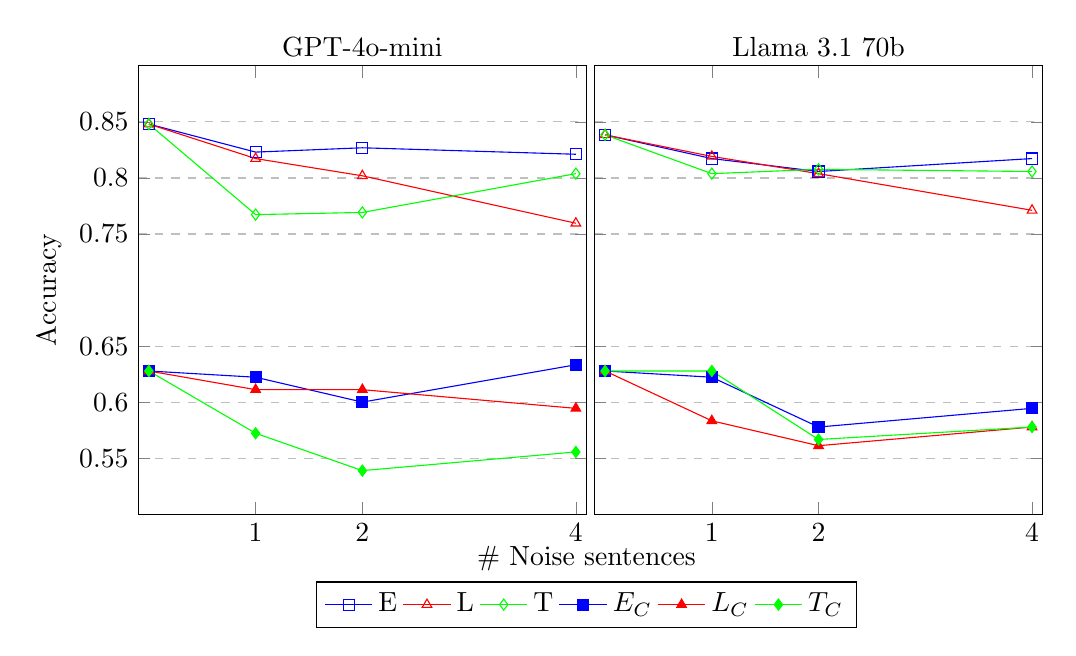
\begin{tikzpicture}
        \begin{axis}[name=gpt,
            title={GPT-4o-mini},
            width=0.6\linewidth,
            height=0.6\linewidth,
            xlabel={\# Noise sentences},
            ylabel={Accuracy},
            xmin=-0.1, xmax=4.1,
            ymin=0.5, ymax=0.9,
            xtick={1,2,4},
            ytick={0.55, 0.6, 0.65, 0.75, 0.8, 0.85},
            title style={yshift=-0.6em},
            legend style={at={(1,-0.15)},
	           anchor=north,legend columns=-1},
            x label style={at={(axis description cs:1,-0.05)},anchor=north},
            y label style={at={(axis description cs:-0.15,0.5)},anchor=south},
            ymajorgrids=true,
            grid style=dashed,
        ]
            \addplot[color=blue, mark=square,]
                coordinates {
                (0,0.848076939582825)(1,0.823076903820038)(2,0.826923072338104)(4,0.821153819561005)
                };
            \addplot[color=red, mark=triangle,]
                coordinates {
                (0,0.848076939582825)(1,0.817307710647583)(2,0.801923096179962)(4,0.759615361690521)
                };
            \addplot[color=green, mark=diamond,] 
                coordinates {
                (0,0.848076939582825)(1,0.767307698726654)(2,0.769230782985687)(4,0.803846180438995)
                };
            \addplot[color=blue, mark=square*] 
                coordinates {
                (0,0.627777755260468)(1,0.622222244739533)(2,0.600000023841858)(4,0.633333325386047)
                };
            \addplot[color=red, mark=triangle*,] 
                coordinates {
                (0,0.627777755260468)(1,0.611111104488373)(2,0.611111104488373)(4,0.594444453716278)
                };
            \addplot[color=green, mark=diamond*,] 
                coordinates {
                (0,0.627777755260468)(1,0.572222232818604)(2,0.538888871669769)(4,0.555555582046509)
                };
                \legend{E,L,T,$\text{E}_C$, $\text{L}_C$ , $\text{T}_C$}
        \end{axis}

        \begin{axis}[name=llama, at={($(gpt.east)+(0.1cm,0)$)},anchor=west,
            title={Llama 3.1 70b},
            width=0.6\linewidth,
            height=0.6\linewidth,
            xmin=-0.1,, xmax=4.1,
            ymin=0.5, ymax=0.9,
            xtick={1,2,4},
            ytick={0.55, 0.6, 0.65, 0.75, 0.8, 0.85},
            title style={yshift=-0.6em},
            yticklabel=\empty,
            ymajorgrids=true,
            grid style=dashed,
        ]
            \addplot[color=blue, mark=square,]
                coordinates {
                (0,0.838461518287659)(1,0.817307710647583)(2,0.805769205093384)(4,0.817307710647583)
                };
            \addplot[color=red, mark=triangle,]
                coordinates {
                (0,0.838461518287659)(1,0.819230794906616)(2,0.803846180438995)(4,0.771153867244721)
                };
            \addplot[color=green, mark=diamond,]
                coordinates {
                (0,0.838461518287659)(1,0.803846180438995)(2,0.807692289352417)(4,0.805769205093384)
                };
            \addplot[color=blue, mark=square*]
                coordinates {
                (0,0.627777755260468)(1,0.622222244739533)(2,0.577777802944183)(4,0.594444453716278)
                };
            \addplot[color=red, mark=triangle*,]
                coordinates {
                (0,0.627777755260468)(1,0.583333313465118)(2,0.561111092567444)(4,0.577777802944183)
                };
            \addplot[color=green, mark=diamond*,]
                coordinates {
                (0,0.627777755260468)(1,0.627777755260468)(2,0.566666662693024)(4,0.577777802944183)
                };
        \end{axis}
    \end{tikzpicture}
    \caption{Influence of the number of noisy sentences for FOL.}
    \label{fig:length_distraction}
\end{figure}



\subsection{Impact of Method Design}
\paragraph{\textbf{\emph{F4: \ac{CoT} prompting is most impactful when both noise and counterfactual perturbations are applied.}}}
The accuracies for the individual \acp{LLM} in Table~\ref{tab:distraction_k4_formalisation} show that the impact of \ac{CoT} is negligible for noise-only datasets (first four columns). Meanwhile, the benefit from \ac{CoT} is most pronounced in the datasets that combine noise and counterfactual perturbations.
The better-performing informal prompting strategy for a model remains stable for all types of distractions. Still, the decline in performance due to counterfactuals leads to a less consistent preference for a specific prompting style.

\paragraph{\textbf{\emph{F5: The best-performing grammar differs per model and is unstable across data versions.}}}

The evaluation of different logical forms for formal \ac{LLM}-based reasoning in Table~\ref{tab:distraction_k4_logical_form} shows the preference of some models for specific syntactic formats.
Llama 3.1 70B has a considerable improvement of $12\%$ with TPTP syntax on the original set, while Llama 3.1 8B benefits from the R-FOL syntax. However, all grammars show a declining accuracy trend and increased syntax errors for noise perturbations, where the best grammar loses its advantage over the rest. 
When comparing the grammars on the counterfactual partitions, we observe that TPTP is consistently more robust than the standard first-order logic grammar. Here, GPT 4o-mini shows a reduction from $O$ to $O_C$ of $20\%$ for FOL and only $12\%$ for the TPTP grammar. Since this does not correlate with fewer syntax errors, the formalisation in TPTP prevents semantical errors for counterfactual premises. 
A positive reading of these results, especially the minor differences between FOL and R-FOL, is that autoformalisation \acp{LLM} can adapt to the grammar syntax prescribed in the prompt without further loss in performance.

\begin{table}[!t]
\small
\setlength{\modelspacing}{2pt}
\setlength{\tabcolsep}{1.7pt} % Default value: 6pt
\setlength{\belowrulesep}{4pt}
\begin{threeparttable}
    \centering
    \begin{tabular}{cc l r rrr @{\quad} rrrr}
\toprule
\multirow{2}{*}{} & \multirow{2}{*}{} & Grammar & \multirow{2}{*}{O} & \multicolumn{3}{c}{Distraction} & \multicolumn{4}{c}{Counterfactual} \\
 & & Syntax & & E& L & T & $\text{O}_C$ & $\text{E}_C$& $\text{L}_C$ & $\text{T}_C$\\
\midrule
\multirow{6}{*}{\rotatebox{90}{Llama-3.1}} & \multirow{3}{*}{\rotatebox{90}{8B}} 
   & FOL & 0.77 & \textbf{0.71} & 0.61 & \textbf{0.53} & 0.58 & \textbf{0.55} & 0.52 & \textbf{0.56} \\
 & & R-FOL & \textbf{0.78} & 0.69 & \textbf{0.62} & \textbf{0.53} & 0.58 & \textbf{0.55} & \textbf{0.54} & 0.52 \\
 & & TPTP & 0.73 & 0.67 & 0.55 & 0.51 & \textbf{0.68} & 0.54 & 0.46 & 0.51 \\[\modelspacing]
\cmidrule{2-11}
 & \multirow{3}{*}{\rotatebox{90}{70B}} 
   & FOL & 0.76 & 0.73 & 0.71 & \textbf{0.72} & 0.67 & 0.57 & 0.63 & 0.56 \\
 & & R-FOL & 0.76 & 0.73 & 0.67 & 0.71 & 0.64 & 0.57 & 0.53 & 0.64 \\
 & & TPTP & \underline{\textbf{0.88}} & \underline{\textbf{0.84}} & \underline{\textbf{0.81}} & \textbf{0.72} & \underline{\textbf{0.81}} & \underline{\textbf{0.68}} & \underline{\textbf{0.67}} & \underline{\textbf{0.68}} \\[\modelspacing]
\midrule
\multirow{3}{*}{\rotatebox{90}{GPT}} & \multirow{3}{*}{\rotatebox{90}{4o-mini}} 
   & FOL & \textbf{0.84} & \textbf{0.82} & \textbf{0.72} & \underline{\textbf{0.78}} & 0.64 & \textbf{0.63} & \textbf{0.61} & 0.51 \\
 & & R-FOL & \textbf{0.84} & 0.77 & 0.70 & \underline{\textbf{0.78}} & \textbf{0.72} & 0.56 & 0.54 & \textbf{0.63} \\
 & & TPTP & 0.83 & \textbf{0.82} & 0.71 & 0.71 & 0.69 & \textbf{0.63} & 0.57 & 0.57 \\
\bottomrule
\end{tabular}
\caption{Accuracies of different formalisation grammars for autoformalisation.}
\label{tab:distraction_k4_logical_form}
\end{threeparttable}
\end{table} 

\paragraph{\textbf{\emph{F6: Feedback does not help \acp{LLM} self-correct to mitigate robustness issues.}}}
\autoref{tab:distraction_k4_feedback} shows the results with different error recovery mechanisms. The results indicate that no feedback strategy emerges as a winner in the different datasets. 
All feedback variants reduce syntax errors for noise perturbations, but given the lack of a consistent increase in accuracy, the corrected formalisations are most likely to contain semantic errors still. 
The type of feedback message only has a minor influence on correcting syntax errors, whereas Llama 3.1 70b and GPT 4o-mini correct slightly more syntax errors with specific error messages. This finding aligns with \cite{huang2023large}, who also found that \acp{LLM} cannot consistently self-correct their reasoning after receiving relevant feedback.

\begin{table}[!ht]
\small
\setlength{\modelspacing}{2pt}
\setlength{\tabcolsep}{1.7pt} % Default value: 6pt
\setlength{\belowrulesep}{4pt}
\begin{threeparttable}
    \centering
    \begin{tabular}{cc l r rrr @{\quad} rrrr}
\toprule
\multirow{2}{*}{} & \multirow{2}{*}{} & \multirow{2}{*}{Feedback} & \multirow{2}{*}{O} & \multicolumn{3}{c}{Distraction} & \multicolumn{4}{c}{Counterfactual} \\
 & & & & E& L & T & $\text{O}_C$ & $\text{E}_C$& $\text{L}_C$ & $\text{T}_C$\\
\midrule
\multirow{8}{*}{\rotatebox{90}{Llama-3.1}} & \multirow{4}{*}{\rotatebox{90}{8B}} 
   & No recovery & 0.77 & \textbf{0.72} & 0.62 & 0.53 & 0.59 & 0.58 & 0.56 & \textbf{0.56} \\
 & & Error type & \textbf{0.79} & 0.71 & 0.63 & \textbf{0.56} & \textbf{0.66} & 0.54 & 0.52 & 0.51 \\
 & & Error message & 0.78 & 0.71 & \textbf{0.67} & 0.55 & 0.59 & 0.53 & \underline{\textbf{0.64}} & 0.49 \\
 & & Warning & 0.74 & 0.66 & 0.58 & 0.55 & 0.55 & \textbf{0.60} & 0.49 & 0.49 \\[\modelspacing]
\cmidrule{2-11}
 & \multirow{4}{*}{\rotatebox{90}{70B}} 
   & No recovery & \textbf{0.77} & \textbf{0.72} & \textbf{0.73} & 0.71 & \textbf{0.64} & 0.59 & \textbf{0.61} & 0.56 \\
 & & Error type & 0.72 & 0.70 & 0.72 & \textbf{0.73} & 0.62 & 0.56 & 0.60 & 0.58 \\
 & & Error message & 0.71 & 0.70 & \textbf{0.73} & 0.71 & \textbf{0.64} & 0.59 & 0.54 & \underline{\textbf{0.64}} \\
 & & Warning & 0.69 & \textbf{0.72} & 0.72 & 0.72 & 0.62 & \underline{\textbf{0.65}} & \textbf{0.61} & 0.63 \\[\modelspacing]
\midrule
\multirow{4}{*}{\rotatebox{90}{GPT}} & \multirow{4}{*}{\rotatebox{90}{4o-mini}} 
   & No recovery & \underline{\textbf{0.84}} & \underline{\textbf{0.82}} & 0.73 & 0.79 & 0.64 & \textbf{0.62} & 0.56 & \textbf{0.56} \\
 & & Error type & 0.83 & 0.79 & 0.74 & 0.76 & 0.67 & 0.57 & 0.56 & \textbf{0.56} \\
 & & Error message & \underline{\textbf{0.84}} & 0.78 & \underline{\textbf{0.77}} & \underline{\textbf{0.80}} & 0.62 & 0.59 & 0.56 & \textbf{0.56} \\
 & & Warning & \underline{\textbf{0.84}} & 0.75 & 0.73 & 0.76 & \underline{\textbf{0.70}} & 0.61 & \textbf{0.61} & 0.55 \\
 \bottomrule
\end{tabular}
\caption{Accuracies of error recovery strategies.}
\label{tab:distraction_k4_feedback}
\end{threeparttable}
\end{table} 

\subsection{Error Analysis}
\label{subsec:errors}
\paragraph{\textbf{\emph{F7: Autoformalisation increases syntax errors for noise perturbations.}}}
The low performance for noise perturbations correlates with more syntax errors for all models and distraction categories (cf. execution rates in Table~\ref{tab:appendix_k4_formalisation_exec}). The three worst-performing models (both Mistral models, Gemma-2 9b) generate, at best, for $37\%$  and, at worst, for only $4\%$ of the samples, a valid logical form.
Gemma-2 9b and Llama3.1 8b produce more syntax errors than the larger counterparts, suggesting that larger models are more robust towards noise perturbations. 
The accuracy of syntactically valid samples is higher than the informal reasoning methods for most distractions (Table~\ref{tab:appendix_k4_formalisation_vacc}), motivating informal reasoning as a backup strategy for formal reasoning. The error message feedback reveals two common syntax errors: 1) errors by models with an initial low execution rate exhibit issues with the template structure, including using incorrect keywords or adding conversational phrases;
2) perturbation-related errors, the most common of which is using undefined truth constants as part of tautological distractions. 

\paragraph{\textbf{\emph{F8: Autoformalisation increases semantic errors for counterfactuals.}}}
Unlike the introduced noise, counterfactual perturbations do not lead to more syntax errors. The execution rate in Table~\ref{tab:appendix_k4_formalisation_exec} is stable or improves for counterfactuals. However, we see a drop in accuracy for the counterfactual column $\text{O}_C$ in Table~\ref{tab:distraction_k4_formalisation} and can conclude that the number of logical forms with semantic errors has to increase. This suggests that the introduced negation is not correctly formalised. Looking at the warnings generated by the feedback mechanism, for GPT 4o-mini, $161$ warning messages are generated on the unperturbed data. $54$ of these were fixed with a single iteration. Not considering predicates and individuals as part of the context is the most frequent warning across all models. 

%%%% DISCUSSION %%%%
\vspace{-0.04in}
\section{Discussion}
\label{sec:discussion}

In this section, we discuss the limitations in current LLM planning research studies, and suggest future directions for improvement and more comprehensive evaluations of LLM planning performance.

\vspace{-0.08in}
\paragraph{Datasets and Baselines} The current evaluation of LLM planning has its limitations, primarily because studies often rely on limited datasets and baselines. This makes it tough to fairly and comprehensively compare different methods. Most studies only use a few datasets from a single domain and difficulty level, and they do not evaluate all the six performance criteria. Inconsistent dataset choices make direct comparisons difficult. On top of that, many studies only compare against basic baselines such as CoT or ReAct, which does not help in comparing more advanced approaches. To fix this, a public, standardized leaderboard should be set up that covers all performance criteria, uses consistent evaluation metrics, includes a variety of baseline and advanced methods, and utilizes diverse datasets spanning multiple domains and difficulty levels. Another useful direction would be to create multilingual planning datasets and assess LLM performance across different languages.

\vspace{-0.08in}
\paragraph{Representation}\; LLMs are highly sensitive to prompts \cite{sclar2024quantifyinglanguagemodelssensitivity, razavi2025benchmarkingpromptsensitivitylarge}, but most research relies on natural language without comparing them to alternative formats, such as PDDL or Python, for describing domains and problems. Some studies \cite{singh2023progprompt, aghzal2024look} suggest that using Python to represent planning problems can improve performance, but automatically translating natural language problem descriptions into Python remains challenging, particularly for non-experts. If LLMs are to handle this translation effectively, additional datasets and evaluations are needed to assess their performance. Furthermore, little research has been conducted on how different prompt templates impact LLM planning performance, or on the best output formats for representing plans. Lastly, most fine-tuning methods rely on natural language data without exploring other formats, such as symbolic representations. Filling these gaps requires building benchmarks like Planetarium \cite{zuo2024planetarium} and carefully choosing representation formats in experiments.

\vspace{-0.08in}
%\vspace{-0.07in}
%\vspace{-0.05in}
\paragraph{Hallucination}  LLMs often experience hallucinations \cite{huang2023survey}, which present two major challenges in planning. First, they might struggle to assess if a plan is achievable given a specific problem description \cite{aghzal2023can, kambhampati2024can}. Second, they can generate inadmissible actions and non-existent objects, requiring translation or expert intervention to correct them \cite{huang2022language, raman2022planning}. This increases the cost of planning systems. Further research is needed to understand the root causes and improve LLMs' ability to accurately identify unachievable plans. Evaluating the impact of these hallucinations remains an important research direction.

\vspace{-0.08in}
%\vspace{-0.07in}
%\vspace{-0.05in}
\paragraph{Human Preference Alignment}\; There is a gap in understanding whether system generated plans align with human preferences. It is crucial for open-ended problems where humans execute the plans. Ensuring alignment with human preferences is vital for safety, feasibility, and usability, particularly in personalized planning tasks such as calendar and travel planning. Additionally, \citet{aghzal2024look} found that LLM planners often fail to achieve optimality in path planning, frequently producing unnecessarily long plans. This may stem from inherent length bias in LLMs, which tend to generate longer sequences. Alignment techniques such as RLHF \cite{ouyang2022training} and DPO \cite{rafailov2024direct} may help alleviate this issue, as humans generally prefer shorter plans for their efficiency, simplicity, and cognitive ease. Further investigation is needed to better align LLM planners with human preferences.

\vspace{-0.07in}
%\vspace{-0.05in}
\paragraph{Cost Effectiveness} Current methods, particularly task decomposition and search-based approaches, often consume a large number of tokens due to lengthy prompts and repeated LLM queries. While heuristic search is considered more efficient than task decomposition, it still requires substantial repeated prompting. To improve cost-effectiveness, we may summarize problem descriptions and enhance heuristic evaluations, e.g., by improving LLM uncertainty estimation \cite{huang2024survey} and verification \cite{li2024systematicanalysisllmcontributions}. These improvements would help reduce prompt length and enable the early stopping of unpromising partial plans.

\vspace{-0.07in}
%\vspace{-0.05in}
\paragraph{Multi-Agent Planning} Most existing research focuses on single-agent planning, where only one agent performs a task. Multi-agent planning \cite{konolige1980multiple, torreno2017cooperative} is more challenging, as it involves multiple agents (e.g., robots) working together or competing in parallel. Despite its complexity, multi-agent planning has received limited attention in AI planning research. It often requires coordinating multiple agents in collaborative or competitive environments where they operate simultaneously. The major challenge lies in developing effective communication protocols and cooperation strategies while generating viable plans for their collective actions.

\vspace{-0.07in}
%\vspace{-0.05in}
\paragraph{Reasoning, Tool Use, and Memory}\quad There is often limited discussion on how other components of LLM agents, such as reasoning, tool use, and memory, affect planning performance. In particular, when LLMs are combined with classical planners or optimizers, it is crucial that the LLM accurately translates the planning problem into the appropriate domain representation to ensure correct plan generation. Currently, these approaches rely on human-selected planners and optimizers. Treating them as tools that LLMs can autonomously choose from could be an exciting prospect. This also raises the question of whether LLMs can effectively select the best tool for a given planning task. Future research should look into enhancing these agentic capabilities in LLM-based planning.




%In this section, we discuss limitations of the current LLM planning work and point out future directions to further enhance and more comprehensively evaluate the LLM planning performance. \hwnote{Need to make the logic in the following paragraphs correct.} 

% The current evaluation of LLM planning is insufficient, due to the limited datasets and baselines used in each study, making it difficult to comprehensively and fairly compare different proposed methods. First of all, most studies use a limited number of datasets with a single domain and difficulty level, and none of them evaluates all six aforementioned performance criteria. Inconsistent datasets choices further hinder direct and fair comparisons. Second of all, many studies only compare against basic baselines, such as CoT and ReAct, making it hard to directly compare more advanced approaches from their reported results. To address these issues, a public, standardized leaderboard should be established. It should incorporate all performance criteria, consistent evaluation metrics, a range of baseline and advanced methods, as well as diverse datasets covering multiple domains, difficulty levels. Another direction is to create multilingual planning datasets and assess LLM performance across languages.%\smallskip

% There is no benchmark that comprehensively evaluates LLM-based planners across all aforementioned six performance criteria. Additionally, most of the examined studies use a limited number of datasets within a single domain and difficulty level. As a result, the reported findings fail to capture all the limitations of the proposed methods, making it challenging for practitioners to select the most suitable approach for their specific needs. Moreover, differences in datasets across studies hinder direct and fair comparisons. Furthermore, many works rely on basic baseline models, such as CoT and ReAct, making it difficult to compare more advanced approaches. Moving forward, a public leaderboard should be established, incorporating all six performance criteria, standardized evaluation metrics, both classical and advanced baseline models, and diverse datasets spanning multiple domains and difficulty levels. \smallskip

% There is no benchmark to comprehensively test LLM-based planners with all the aforementioned six performance criteria. Also, most of the work in the examined papers are using limited number of datasets within a single domain and single difficulty. Thus, the reported results cannot reveal all the limitations of the proposed methods, making it hard for the practitioners to choose which one to use based on their specific needs. Also, Their datasets are also different from other work, making them difficult to compare them directly and fairly. Furthermore, most of the work have very basic baseline models, such as CoT and ReAct, which makes it difficult to compare these more advanced work with each other. In the future, there should be a public leaderboard, with all the six performance criteria, standardized evaluation metrics, both classical and advanced baseline models, and diverse datasets with multiple difficulty and domains. 

% No unified baseline models. Baselines from most of the papers are CoT, ReAct, and ToT, with no advanced developed methods surveyed by this paper.

% Although there are some benchmarks [Embodied interface, PPNL] which target multiple criteria, the datasets and the tasks contained in the benchmark are not diverse enough. 



% The current investigation of input, output, and fine-tuning data representation is insufficient. LLMs are highly sensitive to prompts \cite{sclar2024quantifyinglanguagemodelssensitivity, razavi2025benchmarkingpromptsensitivitylarge}, yet most studies rely solely on natural language representations without comparing alternative formats such as PDDL or Python for describing domains and problems. Some research \cite{singh2023progprompt, aghzal2024look} suggests that using Python to represent problems can improve performance, but the challenge of automatically translating natural language instructions into Python, especially for non-experts, remains unresolved. If LLMs are to be used for this translation, additional datasets and evaluations are needed to assess their effectiveness. Additionally, no studies have explored how different prompt templates affect LLM-based planning performance. Similarly, there is little discussion on the choice of output formats for representing plans, and it remains unclear whether output representation affects planning performance. Finally, most fine-tuning-based methods rely on natural language data without exploring other formats, such as symbolic representations. Addressing these gaps requires both constructing benchmarks like Planetarium \cite{zuo2024planetarium} and carefully selecting representation formats in experiments.

% The current investigation of representation of inputs, outputs and fine-tuning data are not sufficient. LLMs are highly sensitive to prompts \cite{sclar2024quantifyinglanguagemodelssensitivity, razavi2025benchmarkingpromptsensitivitylarge}, yet most studies rely on natural language representations without comparing alternative formats, such as PDDL or Python, for describing domains and problems. Some research \cite{singh2023progprompt, aghzal2024look} suggests that representing problems with Python code can improve performance, but the challenge of translating natural language instructions into Python automatically remains unresolved. If LLMs are to be used for this translation, additional datasets and evaluation are needed to explore their effectiveness. Furthermore, no studies have examined how different prompt templates impact LLM-based planning performance. Similarly, there is little discussion on the choice of output formats for representing plans, and it remains unclear whether output representation affects planning performance. Finally, most of fine-tuning work are using data of natrual language, without explore other formats, such as symbolic representation. All these unknowns deserve further investigation by both constructing the benchmarks like Planetarium \cite{zuo2024planetarium} and carefully choose representation formats during experiments. \smallskip
% LLMs are known sensitive to the prompts. However, most of the work are using natural language representation instead of comparing different representations (such as PDDL, Python) to describe the domain and problems on their tasks. Also, some work found representing plans with Python code can improve the performances, but they did not clearly solve the problem how to convert the natural language instructions into these python code. If we can resort to LLMs, more datasets needs to be developed to test this translation ability. Also, no work discusses the impact of different prompt templates to the performance of the LLM planning. Similar to the inputs, there is no work talking about which output formats should be chosen to represent the plans. It is even unknown if the output representation can actually affect the planning performance. \smallskip

% Inputs (Prompt): 
% What format is the best way to represent the (different) problems? PDDL? Python code? There are only a few studies discussing this (e.g., [Aghzal 2024] for path planning).
% What prompt templates to choose? Since LLMs are very sensitive to the prompt templates, different prompt templates might have different planning performance. 
% If the LLMs can perform better by using formal representation to describe the problem [Aghzal 2024, Pallagani 2023], how should we convert the natural language into these formal representations for non-experts? Can we use another LLM to translate them? How are their performance ⇒ Need more datasets to test this, (e.g. Planetarium [Zuo et al.] for PDDL, but what about other formats, such as Python code?)% Outputs: 



% LLMs suffer from hallucination \cite{huang2023survey}, creating two major challenges in LLM-based planning. First, they struggle to determine whether a given problem is achievable \cite{aghzal2023can, kambhampati2024can}. Second, they generate inadmissible actions and non-existent objects in plans, which needs extra translation and corrections and reduce the efficiency of the planning system \cite{huang2022language, raman2022planning}. Further research is needed to understand the underlying causes of these issues and improve LLM-based planning ability to accurately identify unachievable problems. Additionally, further evaluating the impact of hallucinations on LLM planning remains an important research direction.

%How to further evaluate the hallucination impact on LLM planning is another direction. %\smallskip
% It is known that LLMs suffer from hallucination. In terms of the LLM planning, it causes two problems: fail to identify the achievability of an given problem [Aghzal 2024, ASU o1 paper], and generate nonadmissble actions and non-existing objects in the plans [Huang 2022, Raman 2023]. There is more work to do to investigate why and how these could happen. Also, improving the LLM planning for identifying the unachievable problems is an very important problem.  


% While current LLM planning research focuses on standard evaluation metrics, no work has examined whether the generated plans align with human preferences. This is a crucial question, especially for open-ended problems where humans execute the plans. Ensuring alignment with human preferences is essential for safety, feasibility, and usability. This issue is particularly relevant for personalized planning tasks, such as scheduling (e.g., calendar and travel planning). Additionally, \citet{aghzal2024look} found that LLM-based planners fail to achieve optimality in path-planning problems, often producing unnecessarily long plans. This may stem from an inherent length bias in LLMs, which tend to generate longer sequences. Alignment techniques like RLHF \cite{ouyang2022training} and DPO \cite{rafailov2024direct} could help address this issue, as humans generally prefer shorter plans for their efficiency, simplicity, and cognitive ease. Further investigate is needed for these issues and better align LLM-based planners with human preferences.

% Although the current LLM planning is focusing on the aforementioned evaluation metrics, there is no work focusing on if the output plans are preferred by humans. This is a very important question, especially when the problem is open-ended and the executors are human beings. Also, aligning with Human preference is necessary to make sure all the steps are safe and secure and executable to conduct. Also, this problem is very important to do the personalization planning, especially for task scheduling (e.g., calendar and travel planning). Furthermore, \citet{aghzal2024look} demonstrates that LLM planner cannot achieve the optimality on the path planning problems, ending with outputting unnecessarily long plans. This might be due to the internal length bias of the LLMs, which is they prefer to generate longer sequences than shorter ones. So alignment approaches, such as RLHF and DPO, might be the solution to solve this problem since humans generally prefer shorter plans due to cognitive ease, efficiency, and reduced complexity. \smallskip





% Current approaches, especially task decomposition and search-based methods, often requires significant token consumption due to lengthy prompts and repeated queries. To further improve efficiency, more compact problem descriptions and better heuristic evaluations (e.g., improved LLM uncertainty estimation \cite{huang2024survey} and LLM-verification \cite{li2024systematicanalysisllmcontributions}) should be introduced, which would reduce prompt lengths and enable early-stopping of unpromising partial plans. 

% , also, it is important to excel across many tasks but still faces efficiency bottlenecks. Approaches  How to design better heuristic score function (e.g., model better uncertain) and do the early stopping needs the future investigation. \hwnote{Althgouth heuristic search are more efficient than task decomposition, they still involves hugh amount of repeated prompting.} \smallskip



% Multi-agent planning \cite{konolige1980multiple, torreno2017cooperative}, a classical and more complex AI planning problem, has received limited attention in LLM planning research. Unlike single-agent scenarios, multi-agent planning involves coordinating multiple agents (e.g., robots) that can operate simultaneously and independently. The challenge lies in developing effective cooperation and communication protocols among these agents while generating viable plans for their collective actions.

%Multi-agent planning is a classical problems in the AI planning field, which are very rarely discussed by LLM planning studies. Multiple-agent planning involves multiple agents (e.g., robots) which can operate in parallel and independently, how to make them cooperate and communicate with each other, and plan for this scenario is more challenging than current single-agent scenarios.

% However, most of the examined work are focused on single-agent planning, which means we only plan for one agent (e.g. one robot). Since multiple agents can operate in parallel independently, how to make them cooperate and communicate with each other is more challenging. \smallskip 



% There is limited discussion on how other LLM agent components (i.e., reasoning, tool usage, and memory) impact planning performance. Additionally, while combining LLMs with classical planners or optimizers can ensure correct plan generation if the LLM's translation is accurate, these approaches rely on human-selected planners and optimizers. Treating external planners and optimizers as tools that LLMs can autonomously choose raises the question of whether LLMs can select the most suitable tool based on the given planning problem. Future research should explore improving LLM-based planning by enhancing these agentic capabilities.

% There are limited discussion about the impact of other LLM agent components (i.e., reasoning, tool-use and memory) on its planning abilities. Additionally, although LLM + classical planner / optimizer can guarantee to generate the correct plan if the LLM translation are correct, these work rely on human preselected planners and optimizers. If we consider external planners and optimizers as the external tools which can be used by LLMs, there is more evaluation to see if LLMs can automatically select the appropriate tools based on the planning problems given to them. Thus, the future research can also explore the direction to improving the LLM planning by enhancing other agentic abilities.

%Secondly, there is limited discussion about if improved reasoning abilities and extra internal and external memory can improve the LLM planning abilities. Thus, the future resaerch can also explore the direction to improving the LLM planning by enhancing other agentic abilities.


% First of all, planning requires reasoning abilities, however, there are not a lot of work verifying this and which reasoning methods are the best for LLM planning, given the fact that the most commonly-used reasoning method (i.e., CoT) have limited improvement in limited scenarios. Secondly,  Lastly, like reasoning, there is not a lot of work discussing about the impact of both internal and external memory for the LLM planning abilities. In the future, 

% Firstly, CoT is the most commonly-used reasoning method used in the LLM planning tasks. However, there is no discussion about if this is the best way for LLM planning given the fact that CoT only improves the performance when the human demonstra \citet{} 

% % planning needs reasoning, reasoning and planning are intertwined, which means enhancing reasoning abilities can also improve the planning abilities. However, there is not a lot of work illustrating this. So in the future, we can also test which reasoning methods we should use. Currently, the most common way to do this is CoT and [Stechly 2024] demonstrates the CoT might only depend on a specific prompt engineering to achieve the improvement on the planning tasks. 

% % Reasoning:
% % Since reasoning and planning are intertwined, which means enhancing reasoning abilities can also improve the planning abilities. However, there is not a lot of work illustrating this. So in the future, we can also test which reasoning methods we should use. Currently, the most common way to do this is CoT and [Stechly 2024] demonstrates the CoT might only depend on a specific prompt engineering to achieve the improvement on the planning tasks. 
% External tools:
% When discussing LLM + Classical Planners / Optimizer, no paper is talking about why the specific classical planner or optimizer is used. If we consider these planners and optimizers as a tool, then can LLM automatically choose the optimal or suitable one to use? And also which representation to use? All these are to achieve the fully automatic planning system. 
% Memory
% Although some work exploring the impact of LLM memory for the planning ability, there should be more work exploring this area. Some work talking about this (they talk about how to store the learned successful and failure trajectories and experiences in the memory and facilitate the future planning): “Large Language Models Are Semi-ParametricReinforcement Learning Agents”, “Agent Planning with World Knowledge Mode”.

%\paragraph{Multilingual}






%%%% CONCLUSION %%%%
\section{Conclusion}
% In conclusion, this study highlights the efficacy and potential of integrating Parameter-Efficient Fine-Tuning (PEFT) methods with game theory principles through the innovative approach of LoRA with Mixture of Gamers (\ourmethod). By melding Low-Rank Adaptation (LoRA) with Mixture of Experts (MoE) and utilizing game theory-based dynamics, \ourmethod{} significantly advances the field by addressing critical gaps in flexibility and dynamic expert selection inherent in previous methods. The employment of submatrix decomposition alongside Shapley values in \ourmethod{} enables a more granular understanding of the interactions and contributions of different components within PEFT setups. The promising experimental outcomes across a variety of tasks not only underscore \ourmethod's superior performance but also illuminate its versatile applicability and the potential for future adaptations in complex, domain-specific applications. Moving forward, it will be crucial to refine these approaches, ensuring robustness and scalability, to fully harness the transformative power of PEFT in enhancing machine learning models.

In this paper, we introduce \ourmethod{}, a Med-LVLM that unifies medical vision-language comprehension and generation through a novel heterogeneous knowledge adaptation approach.
% integrates H-LoRA and a three-stage fine-tuning approach, aim at unifying medical understanding and generation tasks. 
% To enhance the multi-task performance of \ourmethod{}, we introduce the \texttt{VL-Health} dataset for training. 
Experimental results demonstrate that \ourmethod{} achieves significant performance improvements across multiple medical comprehension and generation tasks, showcasing its potential for healthcare applications. 

%%%% LIMITATION %%%%
\section{Limitations} \label{sec:limitation}

This work primarily focuses on commonly studied domains involving single-agent scenarios, such as robotics, household tasks, and computer-based tasks. We acknowledge that LLM planning is also applied in other areas, including the natural sciences \cite{o2023bioplanner, liu2024multimodal}, the Internet of Things \cite{cui2024llmind}, and multi-agent scenarios. However, these studies follow similar methodologies and evaluations, suggesting our survey's comprehensiveness. We focus on six commonly used performance criteria and exclude others, such as security and personalization, due to limited research in these areas. Instead, we discuss them in our future directions section.


% Bibliography entries for the entire Anthology, followed by custom entries
%\bibliography{anthology,custom}
% Custom bibliography entries only
\bibliography{custom}


\label{appendix}
% \section{Appendix}
\section{Multimodal Large Language Model}
\label{Appendix_MLLM}
\subsection{Model Innovation}

\label{appendix_MLLM_MI}

\subsubsection{Framework Innovation}

Chaoya Jiang et al.~\cite{jiang2024maven} introduced the multi-granularity hybrid visual encoding framework MaVEn, which combines discrete visual symbol sequences representing abstract, coarse-grained semantic concepts with traditional continuous representation sequences that simulate fine-grained features. This combination enhances the model's ability to understand visual information in images.

Zhuofan Zong et al.~\cite{zong2024mova} proposed the MoVA framework, which incorporates coarse-grained context-aware expert routing and fine-grained expert fusion. This framework adaptively routes and fuses visual experts for specific tasks through a coarse-to-fine mechanism, thereby mitigating the bias of the CLIP visual encoder and enhancing the model's ability to understand and process diverse image content.

Leyang Shen et al.~\cite{shen2024mome} proposed a multimodal expert mixing framework, MoME, which combines the visual expert mixture model (MoVE) and the language expert mixture model (MoLE) to reduce task interference.

Byung-Kwan Lee et al.~\cite{lee2024meteor} proposed the Meteor model, based on the Mamba architecture, which enhances the comprehension and response capabilities of large language and vision models through multifaceted reasoning.

Hao Ma et al.~\cite{ma2024coevolving} proposed the sequential cooperative multi-agent reinforcement learning framework, CORY, which enhances the stability and performance of multimodal large models in reinforcement learning fine-tuning by leveraging the inherent collaborative evolution and emergent capabilities of multi-agent systems.

Yang Jiao et al.~\cite{jiao2024lumen} proposed a vision-centric multimodal large model framework, Lumen, which strengthens multimodal content understanding by decoupling task-agnostic and task-specific learning. This framework enables flexible adaptation to various vision tasks, enhancing the LMM's capabilities in visual perception and instruction following.

Chuyang Zhao et al.~\cite{zhaooctopus} proposed the "Parallel Recognition → Sequential Understanding" MLLM framework, Octopus. This framework achieves parallel recognition of object queries at the lower LLM layers and passes the results to the top LLM layers for sequential understanding, thereby improving the efficiency and accuracy of MLLMs.

Yikai Zhang et al.~\cite{zhang2024wings} proposed the Wings framework, which introduces additional modules and mechanisms to compensate for attention shifts. This allows the model to effectively process visual information while maintaining focus on textual information.

Timin Gao et al.~\cite{gao2024cantor} proposed the Cantor framework, which integrates visual inputs with logical reasoning and leverages the advanced cognitive functions of MLLMs. By acting as a multifaceted expert, it directly acquires higher-level information, thereby improving decision-making quality.

Daqin Luo et al.~\cite{luo2024autom3l} proposed the AutoM3L framework, based on the AutoML architecture, which automates the construction of multimodal training pipelines, feature engineering, and model selection using LLMs, thereby reducing manual intervention.

Yunfeng Fan et al.~\cite{fan2024detached} proposed the DI-MML framework, which addresses modality competition in multimodal learning by independently training modality encoders. They introduced a shared classifier and DUC loss to facilitate cross-modal interaction and knowledge transfer, thereby mitigating the modality competition issue in multimodal learning.

Xinwei Liu et al.~\cite{liu2024multimodal} proposed the multi-step error minimization framework, MEM, which optimizes by combining image noise and text triggers. This approach misleads the model into learning shortcuts, thereby protecting data privacy.

Jinxu Zhang et al.~\cite{zhang2024cream} proposed the CREAM framework, which integrates high-performance retrieval enhancement, multi-image and multimodal processing, and efficient instruction tuning. This effectively addresses the challenges in document-based VQA tasks.

Li Zheng et al.~\cite{zheng2024self} proposed the Adaptive Multimodal Data Augmentation framework, SLUDA, which generates fine-grained data, optimizes the utilization of unlabeled data, and employs adaptive selection strategies and dynamic threshold adjustments. This approach addresses the issues of insufficient labeled data and the underutilization of unlabeled data.

Tao Wu et al.~\cite{wu2024semantic} proposed the SAM model, which enhances semantic associations between images by introducing a bidirectional semantic guidance mechanism. This improves the semantic alignment ability of multimodal instructions.

Shichen Lu et al.~\cite{lu2024collaborative} proposed the Tiny-Large collaborative training framework, CTVLMs, which leverages knowledge distillation and multimodal alignment to enable large models to transfer knowledge to smaller models. This approach achieves a dual improvement in both performance and efficiency.

Minsu Kim et al.~\cite{kim2024efficient} proposed the Bloom framework, which uses bidirectional modality transformation and adaptive cross-modal fusion. It pretrains a VSR (Visual Speech Recognition) model with visual and speech units and introduces a curriculum learning strategy to enhance training efficiency and multilingual recognition performance.

Yunshan Ma et al.~\cite{ma2024cirp} proposed the CIRP framework, which uses a multimodal encoder and cross-item contrastive loss to learn individual item semantics and relationships. By introducing a relationship pruning module, this framework enhances the ability to align cross-modal information and capture cross-item relationships in cold-start items.

Puyi Wang et al.~\cite{wang2024large} proposed the multimodal large model-assisted artificial intelligence-generated image quality assessment framework, MA-AGIQA. By combining multimodal models with traditional DNNs, and utilizing semantic information extraction and a mixture of experts (MoE) structure, the framework dynamically integrates quality perception features. This significantly improves the quality assessment performance of AGIs, particularly excelling in reducing the false-negative rate.

Zhiqi Ge et al.~\cite{ge2024worldgpt} proposed a novel cognitive framework, WorldGPT, which includes memory offloading, knowledge retrieval, and a Context Reflector to enhance the model's performance in specific scenarios and long-term tasks.

Haoning Wu et al.~\cite{wu2023q} proposed the ONEALIGN model, which unifies IQA, IAA, and VQA tasks, thereby enhancing the model's cross-task generalization ability.

Zixin Zhang et al.~\cite{zhangenhancing} proposed the M2FEDSA framework, which combines segmentation learning and multimodal federated learning. By introducing dual-adaptive fine-tuning and dual knowledge transfer strategies, the framework improves both computational and storage efficiency, as well as performance, when deploying large-scale multimodal models in federated learning settings.

Ruisi Cai et al.~\cite{cai2024flextron} proposed an elastic architecture called Flextron, which supports adaptive subnetwork selection. By using routers to choose different sub-models or subnetworks, Flextron addresses the deployment challenges of multimodal large models in resource-constrained environments.

Shengqiong Wu et al.~\cite{wu2023next} proposed an end-to-end Any-to-Any multimodal large model framework, which achieves efficient cross-modal understanding and generation through lightweight alignment techniques and modality-switching instruction tuning.

\subsubsection{Method Innovation}

Xiaotong Li et al.~\cite{li2024densefusion} proposed a comprehensive multimodal perception fusion method that integrates visual experts, thereby enhancing the visual perception capability of MLLMs.

Jiaqing Zhang et al.~\cite{zhang2024e2e} proposed a novel end-to-end algorithm for multimodal fusion detection, achieving high performance through a single training phase and simplifying the overall process.

Junfeng Fang et al.~\cite{fangtowards} proposed a neuron attribution method tailored for MLLMs, called NAM. NAM reveals the modality-specific semantic knowledge learned by neurons in MLLMs and highlights certain neuron characteristics that collectively elucidate the internal workings of MLLMs.

Jayneel Parekh et al.~\cite{parekh2024concept} proposed a concept extraction method based on dictionary learning to interpret the internal representations of large multimodal models. They innovatively defined multimodal concepts and validated their effectiveness in interpreting models and understanding test sample representations.

Junho Kim et al.~\cite{kim2024code} proposed CODE, which utilizes self-generated descriptions as contrastive references to dynamically adjust the information flow, enhancing the coherence and informativeness of responses. This approach addresses the hallucination problem in MLLMs when generating visual content.

Samyadeep Basu et al.~\cite{basu2024understanding} proposed the model editing algorithm MULTEDIT, which can correct errors and insert new information. They also introduced a multimodal causal tracking method, extending the research on information storage to other domains.

Jingjing Xie et al.~\cite{xie2024advancing} proposed the Quantized Scale Learning Method (QSLAW), which effectively reduces quantization errors, prevents overfitting, and improves model adaptability and efficiency by learning the group scale factors of quantized weights and employing a multimodal pretraining strategy.

Yabing Wang et al.~\cite{wang2024multimodal} proposed the MLLM-enhanced cross-lingual, cross-modal retrieval method LECCR. This approach leverages MLLMs to generate visual descriptions, which are then aggregated into multi-view semantic slots to enhance the semantic richness of visual features. By incorporating English feature guidance, it improves the quality of cross-modal alignment.

Zihao Liu et al.~\cite{liu2024adaptively} proposed a visual perception adapter and fine-grained tri-modal contrastive learning method. By aligning tokens across modalities, they reduce semantic gaps, thereby improving the performance of multimodal video tasks.

Weixiang Han et al.~\cite{han2024erl} proposed the ERL-MR strategy, which uses Euler transformations and multimodal constraint loss to transform inter-modal competition into cooperation, thereby achieving performance improvement.

Qiang Wang et al.~\cite{wang2024bilateral} proposed a bilateral adaptive cross-modal fusion prompt learning paradigm, Bloom, which achieves more flexible cross-modal interaction and alignment through bidirectional modal transformation and adaptive fusion functions. This significantly enhances the performance of CLIP on a variety of generalization tasks.

Zongqian Wu et al.~\cite{wu2024adaptive} proposed an adaptive multimodal prompt learning method, AMMPL, which effectively handles meaningless image patches and enhances the model's generalization ability through image prompts and cross-modal interaction learning.

Minghe Gao et al.~\cite{gao2024fact} proposed the Fact paradigm, which teaches MLLMs by generating Faithful, Concise, and Transferable multimodal rationales, enhancing the model's performance and reasoning ability across various visual tasks.

Lincan Cai et al.~\cite{cai2024enhancing} proposed the PaRe method, which enhances the stability and transferability of cross-modal fine-tuning by progressively generating intermediate modalities and replacing modality-agnostic fragments.

Wei Li et al.~\cite{liimproving} proposed the Multimodal Combination Learning (MCL) method, which strengthens the mapping between visual and language modalities. By leveraging LLMs to automatically generate multimodal learning samples, they introduced a stacked retrieval mechanism to extract diverse multimodal information.

Christian Schlarmann et al.~\cite{schlarmann2024robust} proposed the FARE unsupervised adversarial fine-tuning scheme, which enhances the robustness of the CLIP model while preserving its original performance, without the need for retraining on downstream tasks.

Zhuo Huang et al.~\cite{huang2023machine} proposed the DICL strategy, which leverages MLLM knowledge to enhance the robustness of visual models and align MLLMs with visual tasks. This approach enables unsupervised fine-tuning, improving performance in out-of-distribution (OOD) scenarios.

Runpeng Yu et al.~\cite{yu2025attention} proposed the API technique, which enhances model perception through attention heatmaps guided by text queries. This approach enables model self-reflection and integration, improving performance on visual-linguistic tasks and addressing the limitations of traditional visual prompting techniques.

Kai Huang et al.~\cite{huang2025ivtp} proposed the Instruction-guided Visual Token Pruning method (IVTP), which includes an intra-group Token Pruning (GTP) module and cross-modal instruction-guided pruning. This approach effectively reduces the number of visual tokens and lowers computational complexity, while maintaining model performance.



\subsubsection{Module Innovation}



Wenfang Yao et al.~\cite{sun2024chattracker} proposed a novel reflection-based prompt optimization module, leveraging multimodal large language models to generate high-quality language descriptions to improve tracking performance. By iteratively refining the vague and inaccurate descriptions of targets through tracking feedback, this approach addresses the issue of frequent ambiguous language descriptions in annotations.

Zaijing Li et al.~\cite{li2024optimus} proposed a hybrid multimodal memory module that transforms knowledge into a hierarchical directed knowledge graph, enabling agents to explicitly represent and learn world knowledge. Additionally, historical information is summarized into an abstract multimodal experience pool, providing agents with rich contextual learning references. This approach addresses the challenge of general agents struggling to complete long-term tasks in open-world environments.

Jiachen Li et al.~\cite{li2024cumo} enhanced model capabilities by integrating sparse gated Top-K MoE (Mixture-of-Experts) blocks in the visual encoder and MLP connectors, and by introducing MoE blocks during the visual instruction fine-tuning phase. This approach improves the performance of MLLMs on multimodal tasks.

Haogeng Liu et al.~\cite{liu2024visual} innovatively identified visual anchors and proposed a novel vision-language connector, AcFormer. By utilizing visual anchors to aggregate information, this approach significantly enhances the accuracy and computational efficiency of MLLMs.

Ziyuan Huang et al.~\cite{huang2024accelerating} proposed the Chain-of-Sight module, which captures visual details at different spatial scales through a multi-scale visual resampler. This module enables flexible expansion of the number of visual tokens after pretraining, accelerating the pretraining process while maintaining or improving model performance.

Huanjin Yao et al.~\cite{yao2024dense} proposed a new connector, the Dense Connector, which enhances the visual perception ability of MLLMs by integrating multi-layer visual features. It is characterized by high computational efficiency and ease of integration, addressing the issue of existing MLLMs underutilizing the visual encoder while overly emphasizing the language modality.

Haibo Wang et al.~\cite{wang2024weakly} designed the Gaussian Contrastive Localization (GCG) module, which learns to represent the temporal structure of videos and selects key frames relevant to the question. This approach addresses the issue in video question answering where large multimodal models neglect question-related visual cues and lack key timestamp annotations.

Hanzi Wang et al.~\cite{wang2024q} proposed a query-based hybrid expert connector, Q-MoE, which utilizes text-driven routing and an optimal expert path training strategy to achieve precise extraction and processing of task-specific visual information. This approach addresses the issue in MLLMs where the connection structure struggles to filter visual information according to task requirements in vision-language tasks.


\subsection{Benchmarks}

\label{appendix_benchmarks}

\subsubsection{ROPE: Recognition-based Object Probing Evaluation Benchmark}

\label{appendix_rope}

Despite the impressive performance of MLLMs in various downstream applications, they often encounter the issue of object hallucination~\cite{rohrbach2018object,dai2022plausible,li2023evaluating,zhang2024groundhog,zhai2023halle,liu2023mitigating,you2023ferret,zhou2023analyzing,wang2023llm}, where the model erroneously generates objects that do not exist in the image. Current benchmarks for evaluating object hallucination mainly focus on the presence of a single object category, rather than individual entities. 

Xuweiyi Chen et al.~\cite{chen2024multi} conducted a systematic study of the multi-object hallucination problem, examining how models misidentify objects when attending to multiple objects simultaneously (e.g., inventing non-existent objects or being distracted). They introduced an automated evaluation protocol called Recognition-based Object Probing Evaluation (ROPE), which considers the distribution of object categories within a single image during testing. By using visual reference to disambiguate, the protocol systematically analyzes multi-object hallucination, revealing the hallucination behaviors and influencing factors when models process multiple objects. In addition, ROPE designs multiple task prompts, including Default Multi-Object, Student-Forcing, Teacher-Forcing, and Single-Object. The dataset is divided into four subsets, each considering different object category distributions: 1) Homogeneous: All test objects belong to the same category. 2) Heterogeneous: All test objects belong to different categories. 3) In-the-Wild: A mixed object category distribution, with test objects randomly selected and ordered. 4) Adversarial: After multiple repetitions of the same category, a different category object is introduced. The dataset is further divided into Seen and Unseen based on whether the model has encountered these images during instruction tuning. 





More details of the overview of MLLM performance on the  ROPE are provided in table~\ref{rope}.

\begin{table*}[t]
\small
\centering
\caption{Averaged accuracy of baselines on the \textit{In-the-Wild, \textit{Homogeneous}, and \textit{Heterogeneous} splits.} \vspace{3mm}}
\begin{threeparttable}
\begin{tabular}{l|rrr|rrr|rrr|rrr}
\hline
\multicolumn{1}{c|}{\multirow{2}[4]{*}{Model}}
& \multicolumn{3}{c|}{Default Multi-Object}
& \multicolumn{3}{c|}{Student-Forcing}            & \multicolumn{3}{c|}{Teacher-Forcing}            & \multicolumn{3}{c}{Single-Object}             \\
\cmidrule(r){2-4}\cmidrule(r){5-7}\cmidrule(r){8-10}\cmidrule(r){11-13}
% \multirow{-2}{*}{Models}
& Wild
& Hom.
& Het.
& Wild
& Hom.
& Het.
& Wild
& Hom.
& Het.
& Wild 
& Hom.
& Het. \\ 
\hline
% \vspace{0.5mm}
\multicolumn{13}{c}{\textit{Seen}} \\ 
 \hline
Yi-VL-6B~\cite{young2024yi} & 2.95         & 5.65         & 1.99         & 3.44 & 6.80 & 3.78 & 5.45 & 26.25 & 4.36 & 0.19 & 0.30 & 0.13 \\
 
Yi-VL-34B~\cite{young2024yi}                  & 8.50         & 15.35        & 3.33         & 8.97   & 16.30                  & 4.23   & 10.09                  & 19.75   & 4.94   & 0.22   & 2.60   & 0.13   \\
 
LLaVA-7B~\cite{liu2024visual}   & 31.29  & 67.50 & 8.00 & 31.28  & 67.25 & 11.22  & 31.49  & 92.15   & {\color[HTML]{434343} 12.37} & 35.32  & 62.35  & 17.37  \\
 
LLaVA-13B~\cite{liu2024visual}                  & 31.54        & 67.63        & 12.64        & 31.49                  & 73.25                  & 11.54                  & 34.97                  & 94.25   & 16.03                  & 43.13                  & 80.60                  & 23.91                  \\
 
LLaVA-34B~\cite{liu2024visual}                  & 39.95        & 85.75        & 18.85        & \textbf{52.75}             & \textbf{85.20}             & \textbf{33.91}             & \textbf{56.41}             & \textbf{95.81}            & \textbf{25.31}             & 55.05                  & \textbf{86.50}             & 18.97                  \\
\hline
 
Qwen VL~\cite{bai2023qwen}    & 2.73         & 6.60         & 1.03         & 6.25   & 16.00                  & 3.65   & 18.74                  & 71.50   & 5.45   & 8.73   & 16.05                  & 5.58   \\
 
Qwen VL-C~\cite{bai2023qwen}                  & 8.72         & 16.90        & 6.67         & 5.26   & 8.60   & 4.10   & 12.11                  & 47.75   & 8.08   & 25.99                  & 43.40                  & 13.21                  \\
 
CogVLM~\cite{wang2023cogvlm}     & 0.04         & 0.00         & 0.00         & 0.00   & 0.00   & 0.00   & 0.10   & 0.95    & 0.00   & 0.00   & 0.00   & 0.00   \\
 
CogVLM-G~\cite{wang2023cogvlm}   & 0.00         & 0.00         & 0.00         & 9.86   & 13.50                  & 6.79   & 22.64                  & 75.45   & 0.45   & 11.25                  & 22.65                  & 7.12   \\
 
CogVLM-C~\cite{wang2023cogvlm}   & 12.89        & 22.75        & 7.18         & 25.37                  & 43.63                  & 12.03                  & 28.25                  & 72.80   & 17.50                  & 30.16                  & 56.00                  & 16.35                  \\
\hline

LLaVA-7B~\cite{liu2024visual}      &- &- &-   & 9.16               & 16.40              & 5.51        &- &- &-                & 11.68              & 23.55              & 9.36                  \\
GLaMM~\cite{rasheed2024glamm}      &- &- &-   & 27.11        & 53.35        & 13.01        &- &- &-                 & \textbf{63.81}                  & 81.75                  & 53.40                  \\
GroundHOG~\cite{zhang2024groundhog}     &- &- &-   & 23.57              & 30.80              & 24.23        &- &- &-               & 44.80              & 43.10              & 38.97                  \\
\hline
IDEFICS~\cite{laurenccon2024obelics}    & 0.00         & 1.45         & 0.13         & 6.25   & 18.70                  & 0.64   & 17.37                  & 76.15   & 10.06                  & 4.62   & 0.00   & 0.32   \\
IDEFICS~\cite{laurenccon2024obelics}    & 0.00         & 1.45         & 0.13         & 6.25   & 18.70                  & 0.64   & 17.37                  & 76.15   & 10.06                  & 4.62   & 0.00   & 0.32   \\
CogVLM-2~\cite{wang2023cogvlm}   & 21.51        & 37.55        & 17.31        & 37.02                  & 70.85                  & 12.69                  & 37.10                  & 73.50   & 17.44                  & 21.16                  & 38.75                  & 13.65                  \\
MiniCPM-V~\cite{hu2024minicpm}    & 34.75        & 59.91        & 17.37        & 31.62                  & 62.80                  & 13.65                  & 32.16                  & 68.05   & 16.79                  & 27.42                  & 55.35                  & 16.92                  \\
GPT-4V~\cite{achiam2023gpt}     & 53.80        & 77.55        & 40.83       &- &- &-   &- &- &-                 & 55.89                  & 78.25                  & 41.03                  \\
 
GPT-4O~\cite{hurst2024gpt}      & \textbf{71.27} & \textbf{89.25} & \textbf{66.03} &- &- &-   &- &- &-               & 60.77             & 73.92                  & \textbf{54.31}             \\
\hline
LLaVA-7B~\cite{liu2024visual}      & 21.26 & 52.40 & 7.69 &- &- &-   &- &- &-               & 30.59             & 60.85                  & 12.69            \\
+OPERA~\cite{huang2024opera}      & 24.07 & 58.65 & 7.35 &- &- &-   &- &- &-               & 30.44             & 60.85                  & 13.27            \\
\cmidrule(r){1-13}

\multicolumn{13}{c}{\textit{Unseen}} \\    \hline
Yi-VL-6B~\cite{young2024yi} & 2.74         & 3.88         & 1.14         & 3.18   & 4.24   & 5.20   & 4.04   & 10.90   & 10.57                  & 0.14   & 0.45   & 0.08   \\
 
Yi-VL-34B~\cite{young2024yi}                  & 7.77         & 15.63        & 4.23         & 10.28                  & 18.04                  & 7.97   & 11.24                  & 22.49   & 12.03                  & 0.46   & 2.37   & 0.41   \\
 
LLaVA-7B~\cite{liu2024visual}   & 30.56        & 68.12        & 10.33        & 30.55                  & 68.16                  & 10.24                  & 31.89                  & 90.33   & {\color[HTML]{434343} 13.25} & 34.88                  & 64.41                  & 16.18                  \\
 
LLaVA-13B~\cite{liu2024visual}                  & 27.56        & 63.10        & 8.37         & 27.41                  & 63.10                  & 8.37   & 35.65                  & 91.09   & 14.80                  & 42.66                  & 71.92                  & 23.41                  \\
 
LLaVA-34B~\cite{liu2024visual}                  & 29.30        &79.43        & 17.72        & 29.45                  & \textbf{91.18}             & 14.39             & \textbf{37.40}             & \textbf{95.51}            & 17.92                  & 51.71                  & 77.88                  & 30.81                  \\
\hline
 
Qwen VL~\cite{bai2023qwen}    & 2.80         & 1.95         & 7.06         & 7.17   & 16.41                  & 4.15   & 10.34                  & 58.00   & 4.07   & 17.73                  & 31.22                  & 9.51   \\
 
Qwen VL-C~\cite{bai2023qwen}                  & 18.86        & 30.73        & 8.78         & 16.16                  & 27.80                  & 7.72   & 21.81                  & 58.00   & 11.14                  & 34.20                  & 57.31                  & 15.37                  \\
 
CogVLM~\cite{wang2023cogvlm}     & 0.03         & 0.00         & 0.00         & 0.00   & 0.00   & 0.00   & 0.00   & 0.15    & 0.00   & 0.00   & 0.00   & 0.00   \\
 
CogVLM-G~\cite{wang2023cogvlm}   & 0.00         & 0.00         & 0.00         & 8.20   & 1.47   & 5.77   & 23.82                  & 81.20   & 1.81   & 10.32                  & 10.74                  & 9.11   \\
 
CogVLM-C~\cite{wang2023cogvlm}   & 15.56        & 26.57        & 5.53         & 17.18                  & 41.27                  & 6.02   & 22.81                  & 56.04   & 6.67   & 30.56                  & 52.00                  & 13.50                  \\
\hline
LLaVA-7B~\cite{liu2024visual}      &- &- &-  & 7.59               & 12.12              & 4.88       &- &- &-                 & 12.71              & 22.49              & 8.46                  \\
GLaMM~\cite{rasheed2024glamm}      &- &- &-   & 29.11        & 54.53        & 14.23        &- &- &-                & \textbf{68.65}             & 77.06                  & 52.28                  \\
GroundHOG~\cite{zhang2024groundhog}      &- &- &-   & 23.11              & 24.69              & \textbf{26.26}       &- &- &-                & 40.73              & 30.37              & 38.13                  \\
\hline
IDEFICS~\cite{laurenccon2024obelics}    & 0.39         & 0.37         & 0.33         & 9.03   & 24.45                  & 2.68   & 24.80                  & 83.02   & 7.64   & 4.62   & 3.67   & 6.50   \\
CogVLM-2~\cite{wang2023cogvlm}   & 20.99        & 35.06        & 15.93        & 24.64                  & 38.04                  & 23.17                 & 26.74                  & 46.04   & \textbf{26.59}             & 11.13                  & 30.94                  & 5.77   \\
MiniCPM-V~\cite{hu2024minicpm}    & 32.96        & 59.92        & 16.60        & \textbf{31.77}             & 58.98                  & 14.15                  & 31.87                  & 60.98   & 16.34                  & 25.56                  & 47.76                  & 14.39                  \\
GPT-4V~\cite{achiam2023gpt}      & 45.46        & 63.12        & 34.17        &- &- &-   &- &- &-                 & 47.34                  & 64.94                  & 35.45                  \\
 
GPT-4O~\cite{hurst2024gpt}      & \textbf{63.27} & \textbf{80.29} & \textbf{54.47} &- &- &-   &- &- &-                & 63.45                  & \textbf{79.84}             & \textbf{53.74}           \\  
\hline
LLaVA-7B~\cite{liu2024visual}      & 13.96 & 31.88 & 3.98 &- &- &-  &- &- &-                & 26.95                  & 54.41             & 11.06         \\  
+OPERA~\cite{huang2024opera}      & 13.20 & 37.14 & 3.82 &- &- &-   &- &- &-                 & 27.90                  & 56.69             & 11.22         \\  
\hline
\end{tabular}
\end{threeparttable}
% \vspace*{2pt}
\label{rope}
\end{table*}


\subsubsection{CVQA: Culturally-diverse Multilingual Visual Question Answering Benchmark}
\label{appendix_cvqa}


Visual Question Answering (VQA) is a crucial task in MLLMs, designed to test their understanding and reasoning capabilities across visual and textual data~\cite{antol2015vqa, mathew2021docvqa,masry2022chartqa,kafle2018dvqa,chen2021geoqa}. However, most existing VQA datasets primarily focus on English and a few major world languages, with images often being Western-centric. While recent efforts have expanded the linguistic coverage of VQA datasets, they still lack diversity in low-resource languages. Moreover, these datasets typically extend their language range through translation or other methods while keeping the images unchanged, leading to limited cultural representation. To address these limitations, David Romero et al.~\cite{wang2023llm} developed a new benchmark, CVQA, which aims to encompass rich linguistic and cultural diversity. This benchmark involves native speakers and cultural experts in the data collection process to ensure authenticity and inclusivity. 



Figure~\ref{cvqa_fig1} illustrates the scale and diversity of the CVQA benchmark, which includes 10,374 questions and languages from 30 different countries. This demonstrates how it covers a wide range of languages and cultures.


\begin{figure*}[htbp]
    \centering
    \includegraphics[width=0.96\linewidth,height=0.48\linewidth]{fig/cvqa_fig1.png}
    \caption{Statistics of the CVQA Benchmark.~\cite{mathew2021docvqa}}
    \label{cvqa_fig1}
\end{figure*} 


Figure~\ref{cvqa_fig23} shows the performance of different models across various country-language pairs, including question-option pairs in both English and local languages. The blue line in the figure represents performance separated by continents. Despite differences in scale, it highlights the similar behavior of all models in most cases. This figure reveals the challenges models face when handling questions in local languages, as well as the performance variations across different regions and languages.




% 插入两张并排的图片
\begin{figure*}[t]
\centering  %图片全局居中
\subfigure[image 1]{
\label{cvqa_fig2}
\includegraphics[width=0.4\linewidth,height = 0.4\linewidth]{fig/cvqa_fig2.png}}
\subfigure[image 2]{
\label{cvqa_fid3}
\includegraphics[width=0.4\linewidth,height = 0.4\linewidth]{fig/cvqa_fig3.png}}
\caption{Model performance per Country-Language pair. The blue lines indicate separation by continent. All models show similar behaviour in the majority of cases, despite having different sizes.~\cite{mathew2021docvqa}}
\label{cvqa_fig23}
\end{figure*}


Table~\ref{cvqa_tab1} shows the average performance of different MLLMs on the CVQA dataset using English prompts (EN) and local language prompts (LOC). These results indicate that even the best-performing open models, such as LLaVA-1.5-7B, significantly lag behind closed models on CVQA. Furthermore, their performance is poorer with local language prompts, highlighting the challenges models face when processing non-English prompts.


\begin{table*}[htbp]
 \setlength{\tabcolsep}{0pt}
 \renewcommand\arraystretch{1.4}
\centering
\belowrulesep=0pt
\aboverulesep=0pt
\caption{Average performance of MLLMs on our CVQA dataset with English prompts~(EN) and local language prompts~(LOC).~\cite{mathew2021docvqa}}
% \vspace{0.05in}
\resizebox{\textwidth}{!}{
\begin{tabular}{cc|cc|cc|cc|cc|cc|cc|ccccc}
\hline
\multicolumn{2}{c|}{\textbf{LLaVA-1.5-7B}~\cite{liu2024visual}} &\multicolumn{2}{c|}{\textbf{M-CLIP}~\cite{chen2023mclip}} & \multicolumn{2}{c|}{\textbf{CLIP}~\cite{radford2021learning}} & 
\multicolumn{2}{c|}{\textbf{mBLIP-mT0}~\cite{geigle2023mblip}} & \multicolumn{2}{c|}{\textbf{mBLIP-BLOOMZ}~\cite{geigle2023mblip}} & \multicolumn{2}{c|}{\textbf{InstructBLIP}~\cite{dai2023instructblipgeneralpurposevisionlanguagemodels}} &  \multicolumn{2}{c|}{\textbf{Gemini-1.5-Flash}~\cite{team2024gemini}} & \multicolumn{2}{c}{\textbf{GPT-4o}~\cite{hurst2024gpt}} \\
\cmidrule(r){0-2}\cmidrule(r){2-4}\cmidrule(r){4-6}\cmidrule(r){6-8}\cmidrule(r){8-10}\cmidrule(r){10-12}\cmidrule(r){12-14}\cmidrule(r){14-16}
\textbf{EN} & \textbf{LOC} &
\textbf{EN} & \textbf{LOC} &
 \textbf{EN} & \textbf{LOC} & \textbf{EN} & \textbf{LOC} & \textbf{EN} & \textbf{LOC} & \textbf{EN} & \textbf{LOC} & \textbf{EN} & \textbf{LOC} & \textbf{EN} & \textbf{LOC} \\
\hline
49.6 & 35.5 & 38.0 & 33.7 & 42.7 & 30.6 & 31.3 & 30.9 & 39.3 & 32.7 & 49.0 & 31.9 & 66.9 & 68.5 & 75.4 & 74.3 \\
\hline
\end{tabular}
}
\label{cvqa_tab1}
\end{table*}

Table~\ref{cvqa_tab2} compares the performance of LLaVA-1.5-7B and InstructBLIP on CVQA and other established English VQA benchmarks. The results show that while LLaVA-1.5-7B performs better on other English VQA benchmarks, it still faces challenges on CVQA, highlighting the difficulty of culturally specific questions in CVQA.

\begin{table*}[htbp]
\small
\centering
\belowrulesep=0pt
\aboverulesep=0pt
\caption{LLaVA-1.5-7B and InstructBLIP results on various VQA datasets.~\cite{mathew2021docvqa}}
\resizebox{\textwidth}{!}{
\begin{tabular}{l|c|c|c|c|c|c|cccc}
\hline
\textbf{Model} & \textbf{VQAv2} & \textbf{GQA} & \textbf{VizWiz} & \textbf{SciQA-IMG} & \textbf{TextVQA} & \textbf{CVQA~(EN)} & \textbf{CVQA~(LOC)}\\
\hline
LLaVA-1.5-7B~\cite{liu2024visual}& 78.5 & 62.0 & 50.0 & 66.8 & 58.2 & 48.9 & 36.5\\
InstructBLIP~\cite{dai2023instructblipgeneralpurposevisionlanguagemodels} & - & 49.2 & 34.5 & 60.5 & 50.1& 47.8 & 32.7\\
\hline
\end{tabular}}
\label{cvqa_tab2}
\end{table*}


Table~\ref{cvqa_tab3} presents the performance of models across 10 categories in CVQA. It shows that models achieve the highest accuracy in the "People" category, while the accuracy in the "Food" and "Pop Culture" categories is lower with local language prompts. This indicates that the diversity of food and pop culture across different cultures presents a challenge for the generalization of MLLMs.


\begin{table*}[htbp]
\centering
\caption{Accuracy of models across categories.~\cite{mathew2021docvqa}}
\resizebox{1\textwidth}{!}{
\begin{tabular}{@{}l|cc|cc|cc|cc|cc|cc@{}}
\hline
\multirow{2}{*}{\textbf{Categories}} & \multicolumn{2}{c|}{\textbf{LLaVA-1.5-7B}~\cite{liu2024visual}} & \multicolumn{2}{c|}{\textbf{M-CLIP}~\cite{chen2023mclip}} & \multicolumn{2}{c|}{\textbf{CLIP}~\cite{radford2021learning}} & \multicolumn{2}{c|}{\textbf{mBLIP-mT0}~\cite{geigle2023mblip}} & \multicolumn{2}{c|}{\textbf{mBLIP-BLOOMZ}~\cite{geigle2023mblip}} & \multicolumn{2}{c}{\textbf{InstructBLIP}~\cite{dai2023instructblipgeneralpurposevisionlanguagemodels}} \\
\cmidrule(r){2-3}\cmidrule(r){3-5}\cmidrule(r){5-7}\cmidrule(r){7-9}\cmidrule(r){9-11}\cmidrule(r){11-13}
 & \textbf{EN} & \textbf{LOC} & \textbf{EN} & \textbf{LOC} & \textbf{EN} & \textbf{LOC} & \textbf{EN} & \textbf{LOC} & \textbf{EN} & \textbf{LOC} & \textbf{EN} & \textbf{LOC} \\
\hline
Brands & \textbf{49.9} & 36.5 & 37.2& 35.7& 36.6& 29.7& 33.7 & 30.8 & 40.5 & 35.1 & 48.4 & 32.6 \\
Food & \textbf{45.4} & 31.9 & 34.5& 29.1& 39.2& 30.4& 28.1 & 27.6 & 37.7 & 29.8 & 44.4 & 30.6 \\
Geography & \textbf{47.1} & 38.2 & 37.1& 34.2& 41.8& 31.9& 30.6 & 31.6 & 35.0 & 32.3 & 45.3 & 33.2 \\
Objects & 51.8& 33.0& 39.4& 34.5 & 39.7& 25.4& 34.3 & 33.0 & 43.1 & 34.0 & \textbf{52.3}& 29.1 \\
People & 58.9& 38.1 & 45.0& 37.8& 46.8& 30.9& 35.3 & 34.7 & 46.3 & 36.7 & \textbf{59.8}& 34.0 \\
Plants \& Animals & \textbf{55.7}& 37.5 & 43.7& 32.0& 48.0& 27.2& 35.2 & 35.5 & 46.0 & 36.0 & 55.4 & 35.1 \\
Pop Culture & 44.5& 36.3 & 33.7& 31.5& \textbf{46.1}& 36.3& 28.8 & 29.9 & 35.7 & 30.7 & 45.1 & 34.6 \\
Sports & \textbf{50.7} & 39.1& 39.3& 33.3& 43.5& 32.4& 32.6 & 31.4 & 40.1 & 34.9 & 50.5 & 34.7 \\
Tradition & \textbf{50.4} & 35.8 & 37.0& 35.2& 41.9& 32.2& 31.6 & 31.5 & 39.0 & 32.2 & 47.9 & 30.8 \\
Vehicles & 50.6& 41.4& 39.5& 41.1& 44.6& 30.5& 35.6 & 33.9 & 42.0 & 34.0 & \textbf{55.0}& 33.0 \\
\hline
\end{tabular}
}
\label{cvqa_tab3}
\end{table*}


\subsubsection{II-Bench: Image Implication Understanding Benchmark}

\label{appendix_II-Bench}


Images often contain rich emotional and cultural narratives, and understanding their meaning and exploring the human emotions and cultural context they reflect requires attention to detail~\cite{bubeck2023sparks,achiam2023gpt,wachowiak2023does}. While MLLMs have made significant progress in understanding and generating cross-modal content, achieving new breakthroughs in benchmarks like image captioning~\cite{lin2014microsoft,sharma2018conceptual,sidorov2020textcaps,gurari2020captioning,pont2020connecting,agrawal2019nocaps} and visual question answering~\cite{antol2015vqa, mathew2021docvqa, masry2022chartqa,kafle2018dvqa,chen2021geoqa}, there has been insufficient exploration of their higher-order perceptual abilities. Ziqiang Liu et al.~\cite{liu2024ii} introduced a new benchmark, II-Bench, designed to evaluate MLLMs' ability to understand and reason about the complex implicit meanings in images, addressing the gap in existing benchmarks for assessing higher-order perceptual abilities in MLLMs.



II-Bench includes 1,222 images across six different domains: life, art, society, psychology, environment, and others. The images consist of various types, including illustrations, memes, posters, comics, logos, and paintings. Each image is accompanied by one to three multiple-choice questions, totaling 1,434 questions. Of these, 1,399 questions are used to construct the test set, and 35 questions are used for the development and validation sets.

Table~\ref{iibench_tab} presents the overall results of different MLLMs and human participants on the II-Bench benchmark. It shows model performance across various domains, such as life, art, society, psychology, and environment, as well as across different emotional categories (positive, neutral, and negative). The table lists the average and best accuracies for multiple open-source and closed-source MLLMs, alongside the performance of human participants.

\begin{table*}[!thp]
\renewcommand\arraystretch{1.2}
\centering
\caption{Overall results of different MLLMs and humans on different domains and emotions.~\cite{liu2024ii}}
\begin{tabular}{l|c|cccccc|ccc}
\hline
\textbf{Models} & \textbf{Overall} & \textbf{Life} & 
\textbf{Art} & \textbf{Society} & \textbf{Psy.} & \textbf{Env.} & \textbf{Others} & \textbf{Positive} & \textbf{Neutral} & \textbf{Negative} \\
 {} & (1,399) & (585) & (85) & (461) & (152) & (51) & (65) & (196) & (789) & (414) \\
\hline
\multicolumn{11}{c}{\textit{Open-source Models}} \\ 
\hline
InstructBLIP-T5-XL~\cite{dai2023instructblipgeneralpurposevisionlanguagemodels} & 47.3 & 45.6 & 48.2 & 48.8 & 44.7 & 52.9 & 50.8 & 46.9 & 48.3 & 45.4 \\
BLIP-2 FLAN-T5-XL~\cite{li2023blip2} & 52.8 & 53.0 & 58.8 & 52.5 & 42.8 & 64.7 & 58.5 & 56.1 & 52.9 & 51.0 \\
mPLUGw-OWL2~\cite{ye2023mplugowl2} & 53.2 & 54.0 & 56.5 & 50.5 & 52.0 & 60.8 & 56.9 & 55.6 & 52.6 & 53.1 \\
Qwen-VL-Chat~\cite{bai2023qwen}  & 53.4 & 53.2 & 49.4 & 52.1 & 50.0 & 60.8 & 72.3 & 56.1 & 52.6 & 53.6 \\
InstructBLIP-T5-XXL~\cite{dai2023instructblipgeneralpurposevisionlanguagemodels} & 56.7 & 56.2 & 58.8 & 58.6 & 45.4 & 64.7 & 64.6 & 63.3 & 56.1 & 54.6 \\
Mantis-8B-siglip-Llama3 & 57.5 & 56.8 & 61.2 & 57.5 & 53.9 & 64.7 & 61.5 & 59.2 & 58.0 & 55.6 \\
BLIP-2 FLAN-T5-XXL~\cite{li2023blip2} & 57.8 & 57.1 & 63.5 & 57.0 & 53.3 & 66.7 & 66.2 & 67.9 & 57.2 & 54.3 \\
DeepSeek-VL-Chat-7B~\cite{lu2024deepseekvl} & 60.3 & 59.0 & 58.8 & 58.4 & 61.8 & 68.6 & 76.9 & 65.8 & 60.1 & 58.0 \\
Yi-VL-6B-Chat~\cite{young2024yi} & 61.3 & 60.9 & 63.5 & 60.7 & 56.6 & 66.7 & 72.3 & 61.7 & 61.7 & 60.1 \\
InternLM-XComposer2-VL~\cite{dong2024internlmxcomposer2} & 62.1 & 61.7 & 62.4 & 62.3 & 58.6 & 70.6 & 66.2 & 65.8 & 63.0 & 58.7 \\
InternVL-Chat-1.5~\cite{chen2024far} & 66.3 & 63.6 & 65.9 & 68.5 & 65.8 & 64.7 & 76.9 & 73.5 & 65.4 & 64.5 \\
Idefics2-8B~\cite{laurenccon2024obelics} & 67.7 & 67.2 & \textbf{74.1} & 67.7 & 62.5 & 74.5 & 70.8 & 68.9 & 67.0 & 68.4 \\
Yi-VL-34B-Chat~\cite{young2024yi} & 67.9 & 67.5 & 70.6 & 67.7 & 63.8 & 70.6 & 76.9 & 74.0 & 68.2 & 64.5 \\
MiniCPM-Llama3-2.5~\cite{hu2024minicpm} & 69.4 & 68.4 & 71.8 & 69.4 & 64.5 & \textbf{80.4} & 78.5 & 75.0 & 69.3 & 66.9\\
CogVLM2-Llama3-Chat~\cite{hong2024cogvlm2} & 70.3 & 68.9 & 68.2 & 70.9 & 67.8 & 72.5 & \textbf{86.2} & 69.9 & 71.1 & 69.1 \\
LLaVA-1.6-34B~\cite{liu2024visual} & \textbf{73.8} & \textbf{73.8} & 71.8 & \textbf{73.3} & \textbf{71.1} & 78.4 & 81.5 & \textbf{79.1} & \textbf{72.9} & \textbf{72.9} \\
\hline
\multicolumn{11}{c}{\textit{Closed-source Models}} \\ 
\hline
GPT-4V~\cite{achiam2023gpt} & 65.9 & 65.0 & 69.4 & 65.3 & 59.9 & 76.5 & 80.0 & 69.4 & 66.0 & 64.0 \\
GPT-4o~\cite{hurst2024gpt} & 72.6 & 72.5 & 72.9 & 73.3 & 68.4 & 76.5 & 75.4 & 78.6 & 71.2 & 72.5 \\
Gemini-1.5 Pro~\cite{geminiteam2024} & 73.9 & 73.7 & \textbf{74.1} & 74.4 & 63.2 & \textbf{80.4} & 83.1 & \textbf{80.1} & 70.8 & \textbf{75.4} \\
Qwen-VL-MAX~\cite{bai2023qwen} & \textbf{74.8} & \textbf{74.7} & 71.8 & \textbf{74.6} & \textbf{73.0} & 76.5 & \textbf{84.6} & \textbf{80.1} & \textbf{74.5} & 72.9 \\ 
\hline
\multicolumn{11}{c}{\textit{Humans}} \\ 
\hline
Human\_avg~\cite{liu2024ii} & 90.3 & 90.0 & 88.2 & 91.4 & 86.6 & 96.1 & 92.3 & 84.7 & 89.1 & 92.2  \\ 
Human\_best~\cite{liu2024ii} & \textbf{98.2} & \textbf{97.9} & \textbf{98.8} & \textbf{98.3} & \textbf{97.4} & \textbf{100.0} & \textbf{100.0} & \textbf{98.0} & \textbf{98.0} & \textbf{98.8} \\ 
\hline
\end{tabular}%
\label{iibench_tab}
\end{table*}


\subsubsection{ConBench: MLLMs Answer Consistency Evaluation Benchmark}

\label{appendix_ConBench}

MLLMs have made rapid progress in visual information perception and reasoning. Although MLLMs are capable of generating high-quality task prompt responses, simply modifying the prompt can lead to contradictory answers, even when the correct answer is provided. Specifically, under different prompt space sizes, these models lack consistency in answers to the same knowledge point, which significantly undermines trust in these models~\cite{li2023benchmarking,lin2023generating}. To ensure that MLLMs can predict correct and consistent answers when faced with various query formats, Yuan Zhang et al.~\cite{zhang2024unveiling} proposed a multimodal benchmark tool, ConBench, designed to comprehensively assess the consistency of MLLMs—specifically, their ability to provide the same answer to the same knowledge point across different query formats.

ConBench evaluates MLLMs by offering a diverse set of question formats, including true/false questions, multiple-choice questions, and limited visual question answering (VQA) problems. It also introduces two multidimensional evaluation metrics: 1)Discriminative Domain Evaluation Metric (ConScore[D]): Assesses consistency based on the accuracy of the model's answers to discriminative questions. 2)Generative Domain Evaluation Metric (ConScore[C]): Evaluates consistency by comparing the coherence between the model-generated captions and the discriminative answers.




The specific structure of ConBench is shown in figure ~\ref{conbench_fig}, providing an overview of the 19 evaluation categories in ConBench. These categories are distributed across three core capabilities: Sensation, Cognition, and Knowledge. The benchmark comprehensively covers tasks of varying difficulty levels, thereby assessing the performance of MLLMs across different aspects.


\begin{figure}[htbp]
    \centering
    \includegraphics[width=0.9\linewidth,height=0.65\linewidth]{fig/ConBench_fig1.pdf}
    \caption{Overview of 19 evaluation detailed categories in ConBench.~\cite{zhang2024unveiling}}
    \label{conbench_fig}
\end{figure} 


Table~\ref{conbench_tab1} presents the performance evaluation results of different MLLMs on ConBench. These results are based on ConScore[D], which evaluates the correctness of the model's answers to discriminative questions. The table includes three types of questions: True/False (T), Multiple-Choice (C), and Limited Visual Question Answering (VQA) (V). It also shows the models' performance across the three core capabilities: Sensation, Cognition, and Knowledge.


\begin{table*}[t]
  \renewcommand\arraystretch{1.2}
    \centering
	\caption{\textbf{Evaluation[D] of mainstreams series of MLLMs on ConBench.} The detailed results of the Sensation, Cognition, and Knowledge core capabilities are listed below. T, C, and V represent true-false, multiple-choice, and limited VQA questions, respectively. The ranking can be found below the respective numbers. $\dagger$: \scriptsize{Due to safety considerations, GPT-4V declined to answer the celebrity category.}~\cite{zhang2024unveiling}}
	\label{conbench_tab1}
	\scriptsize
        \begin{center}
        \scalebox{1.05}{
	\begin{tabular}{l|c|cccc|cccc|cccc}
	    \shline
	    \multirow{2}{*}{\footnotesize{Method}} & \multirow{2}{*}{\footnotesize{ConScore[D]}} & \multicolumn{4}{c|}{\footnotesize{Sensation}} & \multicolumn{4}{c|}{\footnotesize{Cognition}} & \multicolumn{4}{c}{\footnotesize{Knowledge}}  \\
        \cmidrule(r){3-14}
          & & \multicolumn{1}{c}{\footnotesize{T}} & \multicolumn{1}{c}{\footnotesize{C}} & \multicolumn{1}{c}{\footnotesize{V}} & Con & \multicolumn{1}{c}{\footnotesize{T}} & \multicolumn{1}{c}{\footnotesize{C}} & \multicolumn{1}{c}{\footnotesize{V}} & Con & \multicolumn{1}{c}{\footnotesize{T}} & \multicolumn{1}{c}{\footnotesize{C}} & \multicolumn{1}{c}{\footnotesize{V}} & Con \\
	    \shline
	    \multicolumn{14}{c}{\textit{Closed-source Vision Language Models}}\\
        \hline
            GPT-4V$^\dagger$~\cite{achiam2023gpt}   & $29.20$ & $80.4$ & $79.0$ & $61.7$ & $48.3$ & $68.8$ & $53.2$ & $39.9$ & $20.4$ & $63.1$ & $57.2$ & $30.0$ & $14.2$ \\
            GPT-4-Omni~\cite{hurst2024gpt}  & $35.70$ & $89.2$ & $79.4$ & $64.4$ & $55.0$ & $71.8$ & $62.8$ & $44.9$ & $27.8$ & $64.7$ & $61.7$ & $39.7$ & $23.3$ \\
    	Gemini-Pro-Vision~\cite{geminiteam2024geminifamilyhighlycapable}  & $25.00$ & $85.2$ & $60.7$ & $63.4$ & $39.3$ & $71.8$ & $45.0$ & $44.2$ & $15.1$ & $65.0$ & $51.4$ & $39.7$ & $15.8$ \\
            Gemini-Ultra-Vision~\cite{geminiteam2024geminifamilyhighlycapable}  & $33.10$ & $78.9$ & $78.6$ & $66.3$ & $50.3$ & $68.1$ & $58.5$ & $47.9$ & $28.5$ & $62.9$ & $62.2$ & $44.7$ & $19.7$ \\
            Qwen-VL-Plus~\cite{bai2023qwen}  & $28.10$ & $82.7$ & $74.9$ & $60.4$ & $45.0$ & $64.2$ & $41.7$ & $30.8$ & $16.3$ & $63.6$ & $54.2$ & $33.3$ & $15.8$ \\
            Qwen-VL-Max~\cite{bai2023qwen} & $\mathbf{37.00}$ & $86.4$ & $80.7$ & $65.4$ & $\mathbf{56.3}$ & $72.9$ & $51.4$ & $51.3$ & $28.1$ & $68.3$ & $58.6$ & $38.9$ & $\mathbf{24.2}$ \\
	    \hline
	    \multicolumn{14}{c}{\textit{7B Vision Language Models}}\\
        \hline
            LLaVA-v1.5-7B~\cite{liu2024visual}  & $16.60$ & $79.3$ & $56.8$ & $44.3$ & $28.3$ & $51.4$ & $33.5$ & $15.8$ & $4.7$ & $61.7$ & $44.4$ & $16.9$ & $7.8$ \\
            Qwen-VL-Chat~\cite{bai2023qwen}  & $26.40$ & $81.0$ & $79.6$ & $54.2$ & $39.0$ & $55.0$ & $46.3$ & $33.2$ & $13.5$ & $60.3$ & $54.2$ & $28.9$ & $14.7$ \\
	    \hline
	    \multicolumn{14}{c}{$\sim$ \textit{13B Vision Language Models}}\\
        \hline
            LLaVA-v1.5-13B~\cite{liu2024visual}  & $24.00$ & $82.9$ & $77.1$ & $49.6$ & $39.5$ & $53.6$ & $37.8$ & $20.1$ & $10.4$ & $65.6$ & $50.3$ & $17.2$ & $9.7$ \\
            MiniGemini-13B~\cite{li2024minigemini}  & $21.80$ & $81.9$ & $69.7$ & $52.8$ & $39.3$ & $51.9$ & $38.2$ & $21.1$ & $6.9$ & $52.8$ & $36.7$ & $17.5$ & $9.2$ \\
            InternVL-v1.5-26B~\cite{chen2024far} & $31.40$ & $85.6$ & $84.8$ & $65.0$ & $54.3$ & $59.7$ & $58.6$ & $44.4$ & $19.4$ & $58.1$ & $55.8$ & $25.3$ & $12.2$ \\
	    \hline
	    \multicolumn{14}{c}{$\sim$ \textit{34B Vision Language Models}}\\
        \hline
            LLaVA-NeXT-34B~\cite{li2024llavanextinter} & $27.70$ & $82.4$ & $81.7$ & $55.6$ & $43.6$ & $50.7$ & $47.5$ & $25.6$ & $9.9$ & $60.4$ & $56.1$ & $27.8$ & $12.8$ \\
            MiniGemini-34B~\cite{li2024minigemini} & $23.00$ & $80.8$ & $76.8$ & $48.2$ & $39.7$ & $36.9$ & $30.7$ & $18.9$ & $6.0$ & $58.1$ & $42.3$ & $20.8$ & $8.2$ \\
            InternVL-v1.2P-40B~\cite{chen2024internvl} & $34.70$ & $83.7$ & $83.2$ & $66.6$ & $53.4$ & $74.2$ & $67.6$ & $57.1$ & $\mathbf{34.9}$ & $72.2$ & $58.3$ & $28.6$ & $13.6$ \\

	    \shline
	\end{tabular}
    }
         \end{center}
\end{table*}


Table~\ref{conbench_tab2} further evaluates the consistency between the captions generated by MLLMs and the discriminative answers (ConScore[C]). This includes the overall ConScore[C], as well as consistency scores for the three question types: True/False (T), Multiple-Choice (C), and Limited Visual Question Answering (VQA) (V).


\newcommand{\fg}[1]{\mathbf{\mathcolor{ForestGreen}{#1}}}
\newcommand{\fr}[1]{\mathbf{\mathcolor{Forestred}{#1}}}
\begin{table*}[t]
\renewcommand\arraystretch{1.2}
    \centering
	\caption{\textbf{Evaluation of Consistency between caption and three discriminative types of answer on ConBench.} The Con[$X$] is the Consistency ratio between discriminative answer type $X$ and caption. The "ordered" represents whether Con[T] $<$ Con[C] $<$ Con[V] is in its line.~\cite{zhang2024unveiling}}
	\label{conbench_tab2}
	% \footnotesize
	\scriptsize
	%\normalsize
    \begin{center}
    \scalebox{1.2}{
	\begin{tabular}{l|c|c|cccc}
	    \shline
        \footnotesize{Method} & \footnotesize{ConScore[C]} & \footnotesize{Con[T]} & \footnotesize{Con[C]} & \footnotesize{Con[V]} & \footnotesize{Ordered}\\
	    \shline
	    \multicolumn{6}{c}{\textit{Closed-source Vision Language Models}}\\ \hline
            GPT-4V~\cite{achiam2023gpt}  & 55.6 & $51.20$ & $56.50$ & $59.10$ & Y  \\
            GPT-4-Omni~\cite{hurst2024gpt}  & $\mathbf{62.2}$ & $58.00$ & $62.50$ & $66.10$ & Y \\
            Gemini-Pro-Vision~\cite{geminiteam2024geminifamilyhighlycapable}  & $48.4$ & $43.30$ & $45.20$ & $56.80$ & Y \\
            Gemini-Ultra-Vision~\cite{geminiteam2024geminifamilyhighlycapable} & $54.6$ & $47.80$ & $55.20$ & $60.70$ & Y \\
            Qwen-VL-Plus~\cite{bai2023qwen}  & $50.2$ & $47.10$ & $49.10$ & $54.30$ & Y \\
            Qwen-VL-Max~\cite{bai2023qwen}  & $ 58.4$ & $54.30$ & $58.00$ & $62.90$ & Y \\
	    \hline
    
	    \multicolumn{6}{c}{\textit{7B Vision Language Models}}\\     \hline
            LLaVA-v1.5-7B~\cite{liu2024visual}  & $38.4$ & $39.20$ & $36.60$ & $39.50$ & N\\
            Qwen-VL-Chat~\cite{bai2023qwen}    & $48.0$ & $42.00$ & $50.80$ & $51.30$ & Y\\
	    \hline
	    \multicolumn{6}{c}{$\sim$ \textit{13B Vision Language Models}}\\     \hline
            LLaVA-v1.5-13B~\cite{liu2024visual}   & $44.4$ & $41.50$ & $45.80$& $46.00$ & Y\\
            MiniGemini-13B~\cite{li2024minigemini}  & $41.7$ & $38.80$ & $42.90$ & $43.30$ & Y\\
            InternVL-v1.5-26B~\cite{chen2024far} & $50.9$ & $44.50$ & $53.90$& $54.20$ & Y\\
	    \hline
	    \multicolumn{6}{c}{$\sim$ \textit{34B Vision Language Models}}\\    \hline
            LLaVA-NeXT-34B & $48.3$ & $46.00$ & $52.20$ & $46.80$ & N\\
            MiniGemini-34B~\cite{li2024minigemini}  & $49.6$ & $56.80$ & $48.00$ & $44.10$ & N\\
            InternVL-v1.2P-40B~\cite{chen2024internvl} & $53.7$ & $49.80$ & $55.50$ & $55.80$ & Y\\

	    \shline
	\end{tabular}
    }
         \end{center}
\end{table*}


\subsubsection{COMPBENCH: Comparative Reasoning Benchmark}

\label{appendix_COMPBENCH}



The ability to compare objects, scenes, or situations is crucial for decision-making and problem-solving in everyday life~\cite{masry2022chartqa,hudson2019gqa,lu2022learn}. Although this ability is widespread in human cognition, it has not been fully explored in the field of Artificial General Intelligence (AGI). Jihyung Kil et al.~\cite{kil2024compbench} proposed a benchmark, COMPBENCH, designed to evaluate the comparative reasoning ability of MLLMs.



As show in table~\ref{COMPBENCH_tab1}. COMPBENCH questions are carefully crafted to distinguish relative features between two images, testing the models' performance across eight different comparative dimensions by providing image pairs and related questions. Table~\ref{COMPBENCH_tab2} presents the performance of recent MLLMs on the COMPBENCH benchmark.


\begin{table}[t]
\renewcommand\arraystretch{1.2}
\caption{Overall statistics of COMPBENCH.~\cite{kil2024compbench}}
\setlength{\tabcolsep}{3mm}{
\begin{tabular}{cccc}
\toprule
\multirow{2}{*}{Relativity} & \multirow{2}{*}{Dataset} &\multirow{2}{*}{Domain}  &\multirow{2}{*}{samples}\\ \\
\midrule
\multirow{5}{*}{Attribute} & MIT-States & Open & 0.2K \\
& Fashionpedia & Fashion & 2.4K \\
& VAW & Open & 0.9K \\
& CUB-200-2011 & Bird & 0.9K \\
& Wildfish++ & Fish & 0.9K \\
\cmidrule{1-4}
\multirow{2}{*}{Existence} & MagicBrush & Open & 0.9K \\
& Spot-the-diff & Outdoor Scene & 1.2K \\
\cmidrule{1-4}
\multirow{2}{*}{State} & MIT-States & Open & 0.6K \\
& VAW & Open & 0.5K \\
\cmidrule{1-4}
\multirow{2}{*}{Emotion} & CelebA & Face & 1.5K \\
& FER-2013 & Face & 3.8K \\
\cmidrule{1-4}
\multirow{2}{*}{Temporality} & SoccerNet & Sport & 8.3K \\
& CompCars & Car & 5K \\
\cmidrule{1-4}
Spatiality & NYU-Depth V2 & Indoor Scene & 1.9K \\
\cmidrule{1-4}
Quantity & VQAv2 & Open & 9.8K \\
\cmidrule{1-4}
Quality & Q-Bench2 & Open & 1K \\
\cmidrule{1-4}
Total & - & - & 39.8K \\
\bottomrule
\end{tabular}}
\label{COMPBENCH_tab1}
\end{table}



\begin{table*}[t]
\renewcommand\arraystretch{1.2}
\centering
\caption{Overall results on COMPBENCH test split. Evaluating four leading MLLMs across eight relative comparisons spanning sixteen tasks.~\cite{kil2024compbench}
}
\scalebox{0.9}{
\begin{tabular}{l|ccccc|cc|cc|cc|cc|c|c|c|c}
\hline
\multirow{2}{*}{Model} &
\multicolumn{5}{c|}{Attribute} &
\multicolumn{2}{c|}{Exist.} &
\multicolumn{2}{c|}{State} &
\multicolumn{2}{c|}{Emot.} &
\multicolumn{2}{c|}{Temp.} &
\multicolumn{1}{c|}{Spat.} &
Quan. &
Qual. & 
\multirow{2}{*}{Avg} \\

 \cmidrule(r){2-17}
%\cmidrule(r){2-6} \cmidrule(r){7-8} \cmidrule(r){9-10} \cmidrule(r){11-12} \cmidrule(r){13-14} \cmidrule(r){15-15} \cmidrule(r){16-16} \cmidrule(r){17-17}
& ST & FA & VA & CU & WF & MB & SD & ST & VA & CE & FE & SN & CC & ND & VQ & QB \\
%& MST & FAS & VAW & CUB & WFS & MBR & SPD & MST & VAW & CEA & FER & SCN & COC & NYD & VQA & QBE \\
\hline
GPT-4V~\cite{achiam2023gpt}                  & \textbf{91.8} & \textbf{89.0}    & 76.9 & 71.4 & \textbf{72.1}     & \textbf{58.3} & 41.9      & \textbf{92.2} & \textbf{87.8} & 91.8   & 83.4     & \textbf{71.4} & \textbf{73.7} & 56.1  & \textbf{63.8} & \textbf{73.0}     & \textbf{74.7}                 \\ 
Gemini1.0-Pro~\cite{geminiteam2024geminifamilyhighlycapable}              & 71.9 & 76.3    & 69.3 & 59.9 & 54.9     & 53.7 & \textbf{53.0}      & 81.8 & 70.7 & 60.6   & 71.2     & 55.1 & 58.2 & 56.6  & 54.6 & 59.5     & 63.0                 \\
LLaVA-1.6~\cite{liu2024visual}                & 84.9 & 72.1    & \textbf{77.7} & \textbf{72.6} & 68.7     & 26.5 & 20.7      & 89.7 & 79.3 & \textbf{96.2}   & \textbf{83.5}     & 51.0 & 50.2 & \textbf{67.2}  & 50.1 & 64.8     & 66.0                 \\
VILA-1.5~\cite{lin2024vila}                 & 69.9 & 66.2    & 70.9 & 55.9 & 52.0     & 49.5 & 36.8      & 71.9 & 74.5 & 57.1   & 55.6     & 51.1 & 52.9 & 51.8  & 47.7 & 64.8     & 58.0                 \\
Chance level~\cite{kil2024compbench} & 50.0 & 50.0    & 50.0 & 50.0 & 50.0     & 8.6 & 9.7      & 50.0 & 50.0 & 50.0   & 50.0     & 50.0 & 50.0 & 50.0  & 33.3 & 37.4     & 43.1 \\

\hline
\end{tabular}
}
%\vspace{-12pt}
\label{COMPBENCH_tab2}
\end{table*}

\subsubsection{Hallu-PI: Evaluating Hallucination in Multi-modal Large Language Models within Perturbed Inputs}

\label{appendix_Hallu-PI}

Similarly, in the context of the hallucination problem faced by MLLMs in visual-language understanding and generation tasks~\cite{rohrbach2018object,dai2022plausible,li2023evaluating,zhang2024groundhog,zhai2023halle,liu2023mitigating,you2023ferret,zhou2023analyzing,wang2023llm}, Peng Ding et al.~\cite{ding2024hallu} pointed out that previous studies have mainly focused on evaluating hallucinations on standard, undisturbed benchmarks, neglecting the prevalent interference inputs in the real world. This is crucial for a comprehensive evaluation of hallucinations in MLLMs. They proposed the first benchmark designed to evaluate hallucinations in MLLMs under disturbed inputs, called Hallu-PI, which includes seven types of disturbed scenarios: noise, blur, weather, digits, image stitching, image cropping, and prompt misdirection.


Table~\ref{hallupi_tab1} presents the performance of MLLMs under four basic disturbance types (noise, blur, weather, and digits). The "Before/After" columns compare the performance before and after the perturbation, using the ACC+ (Accuracy+) and CHAIR (Hallucinated Object Occurrence Rate) metrics to measure the level of hallucinations in the models.

\begin{table*}[htbp]
\renewcommand\arraystretch{1.2}
  \centering
  \caption{The results under noise, blur, weather, and digital perturbations. Before/After means before/after perturbation.~\cite{ding2024hallu}}
    \begin{tabular}{l|cc|cc|cc|cc|cc}
   \hline
    \multicolumn{1}{c|}{\multirow{3}[4]{*}{Model}} & \multicolumn{2}{c|}{\multirow{2}[1]{*}{Before}} & \multicolumn{8}{c}{After} \\

     \cmidrule(r){4-11}
          & \multicolumn{2}{c|}{} & \multicolumn{2}{c|}{Noise} & \multicolumn{2}{c|}{Blur} & \multicolumn{2}{c|}{Weather } & \multicolumn{2}{c}{Digital } \\
\cmidrule{2-11}          & \multicolumn{1}{l}{ACC+} & \multicolumn{1}{l|}{CHAIR} & \multicolumn{1}{l}{ACC+} & \multicolumn{1}{l|}{CHAIR} & \multicolumn{1}{l}{ACC+} & \multicolumn{1}{l|}{CHAIR} & \multicolumn{1}{l}{ACC+} & \multicolumn{1}{l|}{CHAIR} & \multicolumn{1}{l}{ACC+} & \multicolumn{1}{l}{CHAIR} \\
    \hline
    CogVLM~\cite{wang2023cogvlm} & \textbf{49.0}  & 62.0    & \textbf{48.5}  & 68.2 & \textbf{47.4} & 68.6 & 42.8 & 67.9 & \textbf{48.4} & 69.8 \\
    Multi-GPT~\cite{achiam2023gpt} & 13.3  & \textbf{73.5}  & 9.6  & 73.6 & 12.8 & \textbf{76.1} & 11.2 & \textbf{73.4} & 9.2  & \textbf{77.8} \\
    LLaVA~\cite{liu2024visual} & 6.3   & 68.5  & 4.33  & 67.7 & 5.0     & 70.6 & 4.17  & 69.8 & 3.6  & 74.2 \\
    LLaVA1.5~\cite{liu2024visual} & 43.0    & 68.9  & 42.6 & 70.1 & 42.4 & 68.7 & 43.3 & 68.0  & 36.8 & 74.5 \\
    MiniGPT-4~\cite{zhu2023minigpt} & 16.0    & 72.4  & 15.8 & 70.2 & 15.9 & 72.1 & 14.5  & 72.6 & 13.8 & 73.9 \\
    MiniGPT4-v2~\cite{chen2023minigpt} & 28.3  & 72.1  & 26.7 & \textbf{74.7} & 28.8 & 74.0  & 28.2 & 72.8 & 27.1 & 74.9 \\
    mPLUG2~\cite{xu2023mplug} & 38.0    & 65.0    & 33.3 & 67.6 & 33.1 & 69.1 & 35.3 & 66.9 & 32.3 & 73.6 \\
    Gemini~\cite{team2023gemini} & 46.0    & 57.3  & 44.2 & 60.0   & 45.1 & 59.7   & 44.8 & 58.5 & 37.5  & 61.3 \\
    GPT-4V~\cite{achiam2023gpt} & 47.3  & 66.1  & 42.3 & 66.9 & 41.8 & 68.4 & \textbf{47.8} & 60.9 & 34.0    & 65.4 \\
    \hline
    \end{tabular}%
  \label{hallupi_tab1}%
\end{table*}%


Table~\ref{hallupi_tab2} focuses on the performance of MLLMs under three additional disturbance types in Hallu-PI: Concat, Cropping, and Prompt Mislead. The PI-Score (a comprehensive evaluation metric) is used to assess the overall performance of the models under these specific disturbance scenarios.

\begin{table}[htbp]
\renewcommand\arraystretch{1.2}
\small
  \centering
  \caption{The results under image concatenation, image cropping, and prompt misleading perturbations.~\cite{ding2024hallu}}
  \setlength{\tabcolsep}{1mm}{
    \begin{tabular}{l|cc|cc|cc}
    \hline
    \multicolumn{7}{c}{PI-Score} \\
    \hline
    \multicolumn{1}{c|}{\multirow{2}[2]{*}{MLLMs}} & \multicolumn{2}{c|}{Concat} & \multicolumn{2}{c|}{Cropping} & \multicolumn{2}{c}{Prompt Mislead} \\
     \cmidrule(r){2-7}
          & \multicolumn{1}{l}{Before} & \multicolumn{1}{l|}{After} & \multicolumn{1}{l}{Before} & \multicolumn{1}{l|}{After} & \multicolumn{1}{l}{Before} & \multicolumn{1}{l}{After} \\
    \hline
    CogVLM~\cite{wang2023cogvlm} & \textbf{45.4}  & 22.5 & 10.0    & 5.0     & 39.6  & 11.4 \\
    Multi-GPT~\cite{achiam2023gpt} & 8.3   & 15.0    & 11.7  & 0.0     & 18.9  & 7.2 \\
    LLaVA~\cite{liu2024visual} & 6.5   & 2.2   & 3.4   & 6.7   & 14.4  & 5.2 \\
    LLaVA1.5~\cite{liu2024visual} & 32.4  & 5.9   & 10.0    & 8.4   & 26.4  & 8.1 \\
    MiniGPT-4~\cite{zhu2023minigpt} & 8.9   & 5.9   & 10.0    & 8.4   & 18.5  & 7.0 \\
    MiniGPT-v2~\cite{chen2023minigpt} & 15.8  & 12.3  & 16.7  & 15.0    & 26.4  & 11.3 \\
    mPLUG2~\cite{xu2023mplug} & 25.7  & 18.9  & 10.0    & 8.3   & 29.7  & 15.7 \\
    InternLM~\cite{cai2024internlm2} & 38.3  & \textbf{37.3}  & 8.3   & 10.0    & 34.4  & 28.0 \\
    Qwen-VL~\cite{bai2023qwen} & 46.3  & 19.6  & 20.0    & 11.7  & 53.2  & 38.2 \\
    VisualGLM~\cite{du2022glm} & 6.8   & 0.6   & 34.0    & 0.0     & 21.2  & 11.3 \\
    Gemini~\cite{team2023gemini} & 44.6  & 21.4  & \textbf{45.0}    & 26.7  & 59.2  & 39.4 \\
    GPT-4V~\cite{achiam2023gpt} & 42.0    & 18.0    & 43.4  & \textbf{30.0}    & \textbf{61.4}  & \textbf{48.2} \\
    \hline
    \end{tabular}
    }
  \label{hallupi_tab2}%
\end{table}%


Table~\ref{hallupi_tab3} provides the performance details of MLLMs in generation tasks under the Concat, Cropping, and Prompt Mislead disturbances. The metrics CHAIR, Cover, Hal, and Cog are used to evaluate the models' performance in generation tasks. These metrics help us understand the models' accuracy and hallucination tendencies when generating descriptions that are consistent with the image content.


\begin{table*}[htbp]
\renewcommand\arraystretch{1.2}
\small
  \centering
  \caption{The results of generative task on image concatenation, cropping, and prompt misleading.~\cite{ding2024hallu}
 }
 \scalebox{0.95}{
    \begin{tabular}{l|cc|cc|cc|cc|cc|cc}
    \hline
    \multicolumn{1}{c|}{\multirow{3}[6]{*}{MLLMs}} & \multicolumn{8}{c|}{Image Concatenation}                      & \multicolumn{2}{c|}{Image Cropping} & \multicolumn{2}{c}{Prompt Misleading} \\
\cmidrule{2-13}          & \multicolumn{2}{c|}{ CHAIR } & \multicolumn{2}{c|}{ Cover } & \multicolumn{2}{c|}{Hal } & \multicolumn{2}{c|}{Cog} & \multicolumn{2}{c|}{Hal} & \multicolumn{2}{c}{Hal} \\
\cmidrule{2-13}          & \multicolumn{1}{l}{Before} & \multicolumn{1}{l|}{After} & \multicolumn{1}{l}{Before} & \multicolumn{1}{l|}{After} & \multicolumn{1}{l}{Before} & \multicolumn{1}{l|}{After} & \multicolumn{1}{l}{Before} & \multicolumn{1}{l|}{After} & \multicolumn{1}{l}{Before} & \multicolumn{1}{l|}{After} & \multicolumn{1}{l}{Before} & \multicolumn{1}{l}{After} \\
    \hline
    CogVLM~\cite{wang2023cogvlm} & 62.0  & 69.0  & 55.3  & 48.3  & 58.3  & 97.1  & 4.3   & 5.9   & 80.0  & 90.0  & 36.7  & \textbf{93.3}  \\
    Multi-GPT~\cite{achiam2023gpt} & 73.5  & \textbf{97.5}  & 22.5  & 2.0   & 96.7  & 86.3  & \textbf{30.8}  & \textbf{77.1}  & 76.7  & \textbf{100.0}  & 63.3  & \textbf{93.3}  \\
    LLaVA~\cite{liu2024visual} & 68.5  & 92.3  & 38.8  & 7.4   & 93.3  & 96.7  & 4.3   & 14.9  & \textbf{93.3}  & 86.7  & \textbf{66.7}  & \textbf{93.3}  \\
    LLaVA1.5~\cite{liu2024visual} & 68.9  & 76.1  & 43.8  & 25.0  & 78.3  & 96.3  & 3.4 & 5.7   & 86.7  & 90.0  & 63.3  & 90.0  \\
    MiniGPT-4~\cite{zhu2023minigpt} & 72.4  & 89.3  & 46.5  & 24.8  & 98.3  & 95.8  & 5.1   & 8.2   & 80.0  & 83.3  & 63.3  & \textbf{93.3}  \\
    MiniGPT-v2~\cite{chen2023minigpt} & 72.1  & 88.9  & 49.6  & 32.5  & \textbf{100.0}  & 96.7  & 4.0   & 7.1   & \textbf{93.3}  & 93.3  & 53.3  & \textbf{93.3}  \\
    mPLUG2~\cite{xu2023mplug} & 65.0  & 82.3  & 44.6  & 14.3  & 86.7  & 89.6  & 6.2   & 6.4   & \textbf{93.3}  & 96.7  & 46.7  & 80.0  \\
    InternLM~\cite{cai2024internlm2} & 58.4  & 79.2  & 16.3  & 9.5   & 71.7  & 62.5  & 18.8  & 16.7  & 86.7  & 86.7  & 43.3  & 63.3  \\
    Qwen-VL~\cite{bai2023qwen}  & 58.2  & 56.3  & 35.8  & 32.3  & 46.7  & 79.2  & 9.8   & 11.1  & 83.3  & 93.3  & 6.7   & 16.7 \\
    VisualGLM~\cite{du2022glm} & \textbf{76.9}  & 89.1  & 45.0  & 29.6  & \textbf{100.0}  & \textbf{99.2}  & 4.4   & 9.2   & \textbf{93.3}  & \textbf{100.0}  & 46.7  & 66.7  \\
    Gemini~\cite{team2023gemini} & 57.3  & 63.4  & 50.2  & 43.7  & 56.7  & 90.8  & 3.6   & 4.5   & 26.7  & 56.7  & 12.1  & 30.0  \\
    GPT-4V~\cite{achiam2023gpt} & 66.1  & 63.6  & \textbf{66.6}  & \textbf{53.6}  & 63.3  & 98.3  & 1.6   & 1.9   & 33.3  & 73.3  & 1.1   & 3.3  \\
    \hline
    \end{tabular}%
    }
  \label{hallupi_tab3}%
\end{table*}%




Table~\ref{hallupi_tab4} presents the performance of MLLMs in discriminative tasks under image stitching, cropping, and prompt misdirection disturbances. The metrics ACC, ACC+, and F1 are used to measure the models' accuracy in discriminative tasks. These data provide insights into the models' ability to handle disturbed inputs in discriminative tasks.


\begin{table*}[htbp]
\renewcommand\arraystretch{1.2}
\small
  \centering
  \caption{The results of discriminative task on image concatenation, cropping, and prompt misleading.~\cite{ding2024hallu} }
  \setlength{\tabcolsep}{1mm}{
    \begin{tabular}{l|ccc|ccc|ccc|ccc|ccc}   
    \hline
    \multicolumn{1}{c|}{\multirow{3}[3]{*}{MLLMs}} & \multicolumn{5}{c}{Image Concatenation} &       & \multicolumn{5}{c}{Image Cropping}    &       & \multicolumn{3}{c}{Prompt Misleading} \\
\cmidrule{2-16}          & \multicolumn{3}{c|}{Before} & \multicolumn{3}{c|}{After} & \multicolumn{3}{c|}{Before} & \multicolumn{3}{c|}{After} & \multicolumn{3}{c}{After} \\

\cmidrule{2-16}
          & \multicolumn{1}{l}{ACC} & \multicolumn{1}{l}{ACC+} & \multicolumn{1}{l|}{F1} & \multicolumn{1}{l}{ACC} & \multicolumn{1}{l}{ACC+} & \multicolumn{1}{l|}{F1} & \multicolumn{1}{l}{ACC} & \multicolumn{1}{l}{ACC+} & \multicolumn{1}{l|}{F1} & \multicolumn{1}{l}{ACC} & \multicolumn{1}{l}{ACC+} & \multicolumn{1}{l|}{F1} & \multicolumn{1}{l}{ACC} & \multicolumn{1}{l}{ACC+} & \multicolumn{1}{l}{F1} \\
    \hline
    CogVLM~\cite{wang2023cogvlm} &  69.9  & \textbf{49.0}  &  74.4  & \textbf{67.2}  & \textbf{42.0}  & \textbf{73.1}  & 50.0  & 0.0   &  66.7  & 50.0  & 0.0   & \textbf{66.7}  & 56.7  & 33.3  & 51.9  \\
    Multi-GPT~\cite{achiam2023gpt} & 46.8  & 13.3  & 52.4  & 41.8  & 16.3  & 48.9  & 48.3  & 0.0   & 65.2  & 45.0  & 0.0   & 62.1  & 28.3  & 6.7   & 41.1  \\
    LLava~\cite{liu2024visual} & 51.5  & 6.3   & 57.2  & 50.3  & 1.0   & 54.0  & 50.0  & 0.0   &  66.7  & 50.0  & 0.0   & \textbf{66.7}  & 1.7   & 0.0   & 3.2  \\
    LLava1.5~\cite{liu2024visual} & \textbf{70.5}  & {43.0}  & \textbf{76.1}  & 51.7  & 8.0   & 61.7  & 51.7  & 6.7   & 56.7  & 48.3  & 6.7   & 45.6  & 40.0  & 3.3   & 5.2  \\
    MiniGPT-4~\cite{zhu2023minigpt} & 43.0  & 16.0  & 47.6  & 30.2  & 7.7   & 25.4  & 38.3  & 0.0   & 55.4  & 30.0  & 0.0   & 46.2  & 20.0  & 0.0   & 33.4  \\
    MiniGPT-v2~\cite{chen2023minigpt} & 55.8  & 28.3  & 56.4  & 48.2  & 21.3  & 41.3  & 55.0  &  26.7  & 62.0  & 48.3  & \textbf{23.3}  & 47.5  & 88.3  & 80.0  & 88.8  \\
    mPLUG2~\cite{xu2023mplug} & 62.3  & 38.0  & 68.3  & 51.5  & 27.3  & 54.5  & 50.0  & 13.3  & 62.5  & 48.3  & 13.3  & 59.7  & 43.3  & 13.3  & 34.6  \\
    InternLM~\cite{cai2024internlm2} & 68.2  & 48.3  & 70.8  &  61.2  & 37.0  & 55.9  & 50.0  & 3.3   & 60.5  &  51.7  & 6.7   & 61.3  & 75.0  & 50.0  & 68.1  \\
    Qwen-VL~\cite{bai2023qwen}  & 62.5  & 39.3  & 62.0  & 55.7  & 18.3  & 52.4  &  58.3  & 23.3  & 65.7  & 48.3  & 16.7  & 53.7  & 93.3 & 86.7  &  92.9  \\
    VisualGLM~\cite{du2022glm} & 46.3  & 5.3   & 50.9  & 43.3  & 0.3   & 45.0  & 50.0  & 0.0   &  66.7  & 50.0  & 0.0   & \textbf{66.7}  & 30.0  & 13.3  & 36.3  \\
    Gemini~\cite{team2023gemini} & 65.7  & 46.0  & 64.1  & 60.0  & 33.7  &  63.2 & {56.7}  & 16.7  & \textbf{67.5}  & 
\textbf{53.3}  & 10.0  & \textbf{66.7}  & 53.3  & 13.3  & 33.3  \\
    GPT-4V~\cite{achiam2023gpt} & 66.7  & 47.3  & 66.1  & 59.8  & 34.3  & 55.8  & \textbf{61.7}  & \textbf{33.3}  &  66.7  & \textbf{53.3}  &  20.0  & 62.5  & \textbf{95.0}  & \textbf{90.0}  & \textbf{94.7}  \\
    \hline
    \end{tabular}}
  \label{hallupi_tab4}%
\end{table*}%

\subsubsection{ReForm-Eval: Evaluating MLLMs via Unified Re-Formulation of Task-Oriented Benchmarks}

\label{appendix_ReForm-Eval}

MLLMs have made significant progress in understanding and reasoning about visual information~\cite{achiam2023gpt,zhu2023minigpt,liu2024visual,ye2023mplug,chen2023shikra}. However, this has posed challenges for the automatic evaluation of free-form text outputs from MLLMs. To leverage annotations from existing benchmarks and reduce the manual effort required to construct new benchmarks, Zejun Li et al.~\cite{li2024reform} proposed a method for reformatting existing benchmarks into a unified format compatible with MLLMs. Through systematic data collection and reformatting, they introduced the ReForm-Eval benchmark, which is designed to comprehensively and quantitatively assess the capabilities of MLLMs. This approach overcomes the structural differences between existing task-oriented multimodal benchmarks and MLLMs.


Figure~\ref{reform_eval_fig} illustrates the capabilities and task dimensions of the ReForm-Eval benchmark. It categorizes the evaluation dimensions into two major categories with eight subcategories: 1)Visual Perception Tasks: Coarse-Grained Perception (CG), Fine-Grained Perception (FG), Scene Text Perception (STP). 2)Visual Cognition Tasks: Visually Grounded Reasoning (VGR), Spatial Understanding (Spatial), Cross-Modal Inference (CMI), Visual Description (Desc), Multi-Turn Dialogue (Dialog).

These categories and subcategories comprehensively cover different aspects of MLLMs' visual understanding and reasoning capabilities, providing a comprehensive benchmark  for evaluating model performance.

\begin{figure}[htbp]
    \centering
    \includegraphics[width=0.9\linewidth,height=0.9\linewidth]{fig/reform_eval.pdf}
    \caption{Assessed capability dimensions and tasks in ReForm-Eval. ''Desc'' and ''Classif'' are respectively short for description and classification.~\cite{li2024reform}}
    \label{reform_eval_fig}
\end{figure} 


Table~\ref{reform_eval_tab} shows a comprehensive performance evaluation of 16 open-source MLLMs across different capability dimensions, based on the ReForm-Eval benchmark.


\begin{table*}[t]
\renewcommand\arraystretch{1.2}
    \centering
        \caption{General evaluation results of MLLMs across different capability dimensions. ``CG'', ``FG'', ``CMI'', and ``Desc'' are respectively short for coarse-grained perception, fine-grained perception, cross-modal inference, and description. ``$\bar{R}$'' represents the average rank across dimensions.~\cite{li2024reform}}
    \resizebox{\textwidth}{!}{
    \begin{tabular}{c|ccc|ccccc|c|cc|cccc|c}
    \hline
    &  \multicolumn{9}{c}{\textbf{Generation Evaluation}}
    &  \multicolumn{7}{c}{\textbf{Likelihood Evaluation}} \\ \cmidrule{2-17}  
    \textbf{Model}
    & \multicolumn{3}{c|}{\textbf{Perception}}
    & \multicolumn{5}{c|}{\textbf{Cognition}} 
    & \multirow{2}{*}{$\bar{R}$}
    & \multicolumn{2}{c|}{\textbf{Perception}}
    & \multicolumn{4}{c|}{\textbf{Cognition}} 
    & \multirow{2}{*}{$\bar{R}$}  \\  \cmidrule{2-9}  \cmidrule{11-16}  
    & CG & FG & STP  & Spatial & VGR  & Dialog & CMI & Desc 
    &    & CG & FG   & Spatial & VGR  & Dialog & CMI &  \\ \midrule
    $\text{BLIP-2}_F$~\cite{li2023blip} 			& 69.4 & 76.6 & 38.1  & 43.2 & 73.3 & \textbf{61.8} & 66.9 & \textbf{74.3} & 2   & 60.7  & 74.4  & 51.1  & 69.8  & 62.6  & 58.9 & 4 \\
    $\text{InstructBLIP}_F$~\cite{dai2023instructblip}		& \textbf{71.2} & \textbf{78.1} & \textbf{41.2}  & \textbf{46.1} & \textbf{73.9} & 60.6  & \textbf{71.4} & 43.8 & \textbf{2}   & 60.4  & 75.6  & 51.2  & 71.0  & 67.2  & 55.5 & 4 \\
    $\text{InstructBLIP}_V$~\cite{dai2023instructblip} 	& 69.1 & 70.8 & 40.7  & 44.4 & 63.0 & 48.6  & 53.8 & 27.3 & 4   & 58.5  & 77.8  & 52.3  & \textbf{73.5}  & \textbf{68.7}  & 55.4 & 3 \\
    $\text{LLaVA}_V$~\cite{liu2024visual}  			& 28.7 & 34.4 & 18.4  & 28.7 & 44.0 & 35.6  & 47.3 & 36.8 & 11  & 61.0  & 70.3  & 42.4  & 58.9  & 52.3  & 48.0 & 8 \\
    $\text{LLaVA}_{L_2}$~\cite{liu2024visual}  		& 48.3 & 59.8 & 21.5  & 41.2 & 59.7 & 46.3  & 49.9 & 39.5 & 6   & 49.9  & 65.6  & 47.4  & 56.7  & 48.6  & 49.7 & 11 \\
    MiniGPT4~\cite{zhu2023minigpt}					& 46.2 & 53.2 & 33.0  & 34.6 & 45.6 & 39.5  & 45.4 & 47.5 & 7   & 54.9  & 70.6  & 49.2  & 57.3  & 54.1  & 50.9 & 8 \\
    mPLUG-Owl~\cite{ye2023mplugowl2} 					& 42.0 & 37.2 & 39.8  & 26.8 & 37.5 & 35.2  & 40.4 & 44.7 & 11  & 57.9  & 66.1  & 48.6  & 54.3  & 45.5  & 49.8 & 10 \\
    PandaGPT~\cite{su2023pandagpt}					& 28.2 & 34.6 & 4.5   & 33.3 & 41.9 & 34.1  & 36.6 & 1.6  & 14  & 42.3  & 47.4  & 39.4  & 43.3  & 41.5  & 37.0 & 16 \\
    IB-LLM~\cite{han2023imagebind}					& 29.2 & 32.7 & 8.2   & 35.6 & 36.7 & 35.3  & 36.6 & 27.6 & 13  & 49.6  & 54.4  & 46.1  & 50.3  & 39.5  & 45.6 & 15 \\
    LA-V2~\cite{gao2023llama}						& 33.2 & 30.8 & 24.2  & 23.8 & 36.3 & 35.4  & 41.1 & 36.0 & 13  & 42.7  & 61.4  & 48.6  & 54.1  & 43.4  & 49.9 & 12 \\
    mmGPT~\cite{gong2023multimodal}						& 30.4 & 30.3 & 16.7  & 26.9 & 33.0 & 31.8  & 38.2 & 27.7 & 14  & 52.6  & 62.4  & 47.2  & 56.2  & 43.1  & 44.1 & 13 \\
    Shikra~\cite{chen2023shikra}						& 47.2 & 47.5 & 8.3   & 33.3 & 41.2 & 35.2  & 44.5 & 31.8 & 11  & 60.9  & 66.8  & 45.5  & 58.5  & 59.5  & \textbf{59.3} & 7 \\
    Lynx~\cite{zeng2024matters}						& 59.5 & 62.6 & 18.6  & 40.2 & 58.4 & 47.0  & 53.0 & 60.7 & 5   & \textbf{66.1}  & 76.2  & \textbf{53.9}  & 69.9  & 60.0  & 57.4 & 3 \\
    $\text{Cheetor}_V$~\cite{li2023empowering} 			& 52.0 & 50.3 & 25.9  & 30.6 & 49.9 & 40.3  & 47.4 & 61.6 & 7   & 56.1  & 69.0  & 48.4  & 58.7  & 57.6  & 50.6 & 8 \\
    $\text{Cheetor}_{L_2}$~\cite{li2023empowering}		& 46.5 & 51.4 & 18.8  & 34.5 & 54.4 & 40.6  & 44.0 & 43.9 & 8   & 61.6  & 56.1  & 48.7  & 57.5  & 46.8  & 47.2 & 11 \\
    BLIVA~\cite{hu2024bliva}						& 41.7 & 43.4 & 40.8  & 33.3 & 42.4 & 39.8  & 45.2 & 52.5 & 8   & 64.9  & \textbf{78.2}  & 51.7  & 72.9  & 68.1  & 53.7 & \textbf{2}     
    \\ \hline
    \end{tabular}}
    \label{reform_eval_tab}
\end{table*}

\subsubsection{VisionGraph: Graph Theory Problems Benchmark in Visual Context}

\label{appendix_VisionGraph}


MLLMs have achieved significant success in visual understanding and reasoning~\cite{luo2023wizardmath,liu2024visual,chen2023shikra,achiam2023gpt}, but multimodal graph reasoning remains a challenging task~\cite{wang2024can}. It requires MLLMs to accurately understand graph structures and perform multi-step reasoning on visual graphs. To explore the ability of advanced MLLMs to address multimodal graph reasoning tasks, Yunxin Li et al.~\cite{li2024visiongraph} designed a benchmark called VisionGraph, which includes a series of graph reasoning problems aimed at testing MLLMs' understanding of graph structures and their multi-step reasoning capabilities.


Table~\ref{VisionGraph_tab1} presents the performance of different MLLMs on the VisionGraph benchmark, including evaluation metrics such as node recognition accuracy, edge recognition accuracy, and solution accuracy for specific graph theory problems. These results provide valuable insights for researchers into the models' abilities to understand and reason about graph structures.


\begin{table*}[t]
\renewcommand\arraystretch{1.20}
\caption{MLLMs results in the VisionGraph benchmark.~\cite{li2024visiongraph}}
\label{VisionGraph_tab1}
\centering
\scriptsize
\scalebox{0.95}{
\begin{tabular}{l|ccccccccc}
\hline
Model$\downarrow$ Task Types $\rightarrow$ & Connect & Cycle & Topo. Sort & Shortest Path & Max. Flow & Bipartite Graph & Hamilton Path & GNNs \\ 
\hline
 & \multicolumn{9}{c}{\textit{Node Recognition}} \\
\hline
%MiniGPT-4 $^{\clubsuit}$(Vicuna-7b, T=1.0) & 19.41 & 16.75 & 36.30 & 37.50 & 29.31 & 9.52 & 43.10 & 41.03 & \\
MiniGPT-4 (Vicuna-7b)~\cite{zhu2023minigpt} & 19.14 & 12.04 & 42.96 & 42.19 & 32.76 & 8.33 & 60.34 & 53.85 & \\
BLIP-2 (FlanT5-xxl)~\cite{li2023blip} & 37.74 & 52.88 & 47.41 & 81.25 & 67.24 & 22.62 & 62.07 & 61.54 &  \\
%mPLUG-Owl$^{\clubsuit}$ (Vicuna-7b) \\
%mPLUG-Owl$^{\clubsuit}$ (V-4-shot) \\
InstructBLIP (FlanT5-xl)~\cite{dai2023instructblip} & 36.12 & 47.64 & 46.67 & 75.00 & 56.90 & 36.90 & 53.45 & 74.36 & \\
InstructBLIP (FlanT5-xxl)~\cite{dai2023instructblip} & 35.31 & 52.88 & 61.48 & 85.94 & 77.59 & 17.86 & 65.52 & 61.54 &  \\
Sphinx~\cite{lin2023sphinx}  &	61.99	&98.95	&94.07&	100.00	&91.38	&55.95	&\textbf{100.00}&	97.44\\
Internlm~\cite{cai2024internlm2}  &	\textbf{67.92}	& \textbf{100.00}	&\textbf{97.78}	&\textbf{100.00}	&\textbf{98.25}	&\textbf{77.38}	&\textbf{100.00}	&\textbf{100.00}\\
Llava-v1.5-7b~\cite{liu2024visual}  &   64.15 & 96.86 & 92.59 & 100.00 & 93.10 & 13.10 & \textbf{100.00} & 94.87 \\
Llava-v1.5-13b~\cite{liu2024visual}  &   62.26 & 97.91 & 91.11 & 100.00 & 96.55 & 11.9 & \textbf{100.00} & 97.44 \\
Qwen-Plus (0-shot)~\cite{bai2023qwen}	& 2.96	&0.00	&0.00	&0.00	&5.17&	0.00	&0.00	&56.41\\
Qwen-max (0-shot)~\cite{bai2023qwen}	&29.11	&31.94	&30.37&	12.50	&3.45	&14.29	&29.31	&46.15\\
Gemini (0-shot)~\cite{geminiteam2024geminifamilyhighlycapable} &  40.97 & 42.93 & 47.41 & 67.19 & 72.41 & 10.71 & 65.52 & 35.90 \\
GPT-4V (0-shot)~\cite{achiam2023gpt} &   46.49 & 81.15 & 81.48 & 89.06 & 58.62 & 20.24 & 100.00 & 97.44 \\
\hline


& \multicolumn{9}{c}{\textit{Edge Recognition (Correct / Error)}} \\
\hline
MiniGPT-4 (Vicuna-7b)~\cite{zhu2023minigpt} & 11.78/31.78 & 0.68/1.59 & 12.54/58.89 & 4.78/87.20 & 0.61/61.15 & 14.45/47.53 & 28.48/34.69 & 37.48/55.05 & \\
BLIP-2 (FlanT5-xxl)~\cite{li2023blip} & 12.49/84.03 & 15.11/84.69 & 0.08/2.14 & 1.75/96.84 & 0.00/0.00 & 9.92/75.89 & 11.73/45.55 & 17.26/\textbf{88.84} & \\
Sphinx ~\cite{lin2023sphinx}	&44.76/66.69	&22.13/79.69	&37.84/73.07	&39.88/70.62	&20.68/86.57	&\textbf{83.93}/53.51	&66.26/71.15	&60.66/61.43\\
Internlm ~\cite{cai2024internlm2} &53.08/35.01&	40.78/60.05&	\textbf{55.70}/50.85	&\textbf{57.82}/45.02	&\textbf{23.45}/80.27	&71.21/42.34	&\textbf{73.98}/36.00	&\textbf{83.00}/19.69\\
InstructBLIP (FlanT5-xl)~\cite{dai2023instructblip} & 17.24/\textbf{87.62} & 26.02/\textbf{88.06} & 0.00/0.00 & 5.70/93.93 & 0.00/0.00 & 12.72/83.13 & 37.07/\textbf{82.85} & 49.18/81.28 & \\
InstructBLIP (FlanT5-xxl)~\cite{dai2023instructblip} & 16.34/81.50 & 16.04/85.54 & 0.00/0.00 & 3.58/\textbf{98.31} & 0.00/0.00 & 13.26/\textbf{76.86} & 32.05/65.84 & 37.70/67.57 & \\
Llava-v1.5-7b~\cite{liu2024visual}    & 46.81/58.13 & 23.23/77.63 & 36.56/72.97 & 38.76/66.47 & 9.80/91.56 & 63.10/54.70 & 80.14/48.06 & 69.85/32.92 \\

Llava-v1.5-13b~\cite{liu2024visual}    & 51.18/53.41 & 22.60/76.91 & 38.80/70.26 & 41.93/63.50 & 9.89/91.72 & 67.88/54.21 & 76.26/45.21 & 67.40/33.59 \\

Qwen-Plus~\cite{bai2023qwen}	&30.46/64.78	&27.42/82.37	&10.59/68.46&	6.16/81.60	&1.32/64.62	&75.93/58.65	&48.63/50.41	&33.71/60.56 \\
Qwen-max~\cite{bai2023qwen}	& 25.71/63.21&	20.92/83.50&	16.70/\textbf{76.00}	&1.63/95.70	&1.12/\textbf{96.58}	&42.59/55.55&	40.47/51.61&	35.17/55.81\\
Gemini (0-shot)~\cite{geminiteam2024geminifamilyhighlycapable}  & 23.26/52.35 & 21.65/80.09 & 19.11/66.94 & 16.18/83.09 & 4.79/94.78 & 66.01/53.90 & 39.40/37.80 & 40.83/52.60 \\
GPT-4V (0-shot)~\cite{achiam2023gpt}   & 14.10/23.09 & 17.50/72.97 & 9.64/30.58 & 23.01/66.85 & 5.31/43.62 & 24.13/32.33 & 29.22/38.03 & 46.14/42.74 \\
GPT-4V (4-shot)~\cite{achiam2023gpt}  & 20.63/34.52 & 26.25/69.95 & 13.19/51.75 & 23.40/61.90 & 6.12/84.94 & 46.33/51.69 & 58.49/49.79 & 48.06/35.01 \\
\hline


 & \multicolumn{9}{c}{\textit{Accuracy on Specific Graph Theory Problems}} \\
\hline
%MiniGPT-4 $^{\clubsuit}$(Vicuna-7b, T=1.0) & 54.45 & 51.83 & 0.00 & 0.00 & 0.00 & 1.19 & 0.00 & 0.00 \\
MiniGPT-4 (Vicuna-7b)~\cite{zhu2023minigpt} & 50.67 & 48.69 & 0.00 & 0.00 & 0.00 & \textbf{5.95} & 0.00 & 0.00 \\
BLIP-2 (FlanT5-xxl)~\cite{li2023blip} & 46.63 & \textbf{61.26} & 0.00 & 0.00 & \textbf{13.79} & 0.00 & 0.00 & 0.00 \\
%mPLUG-Owl$^{\clubsuit}$ (Vicuna-7b) \\
%mPLUG-Owl$^{\clubsuit}$ (V-4-shot) \\
InstructBLIP (FlanT5-xl)~\cite{dai2023instructblip} & 48.79 & 47.12 & 0.00 & 0.00 & 6.90 & 0.00 & 0.00 & 0.00 \\
InstructBLIP (FlanT5-xxl)~\cite{dai2023instructblip} & 48.25 & 52.88 & 0.00 & 0.00 & 12.07 & 0.00 & 0.00 & 0.00 \\
Llava-v1.5-7b~\cite{liu2024visual}     & 53.37 & 47.12 & 0.00 & 3.12 & 1.72 & 0.00 & 0.00 & 0.00\\

Llava-v1.5-13b~\cite{liu2024visual}   & 52.83 & 47.12 & 0.00 & 4.69 & 3.45 & 0.00 & 0.00 & 0.00\\

 Gemini (0-shot)~\cite{geminiteam2024geminifamilyhighlycapable}  & 55.52 & 48.69 & 0.00 & 0.00 & 3.45 & 1.72 & 0.00 & 0.00 &\\
GPT-4V (0-shot)~\cite{achiam2023gpt}  & 38.81 & 49.21 & - & 3.12 & - & - & 0.00 & -\\
GPT-4V (2-shot)~\cite{achiam2023gpt}  & 54.98 & 52.35 & - & 6.25 & - & - & 0.00 & -\\
GPT-4V (0-COT)~\cite{achiam2023gpt}  & 30.45 & 50.26 & - & \textbf{7.69} & - & - & 0.00 & -\\
GPT-4V (2-COT)~\cite{achiam2023gpt}  & 54.71 & 52.87 &  -& 6.25 & - & - & 0.00 & -\\

%\\没有GPT-4V (4-shot)
\hline
\end{tabular}
}
\end{table*}


Table~\ref{VisionGraph_tab2} shows the performance improvements of models on three representative graph theory problems (Connectivity, Cycle, and Shortest Path) after applying the Description-Program-Reasoning (DPR) method. The DPR approach enhances MLLMs' multi-step reasoning abilities by combining natural language processing and programming logic.

\begin{table*}[t]
\renewcommand\arraystretch{1.2}
\caption{Model performance on three common graph theory problems in VisionGraph.  ~\cite{li2024visiongraph}}
\label{VisionGraph_tab2}
\centering
\scriptsize
\begin{tabular}{l|cccc|cccc|ccc}
\hline
Task Types $\rightarrow$ & \multicolumn{4}{c|}{Connectivity } & \multicolumn{4}{c|}{Cycle } & \multicolumn{3}{c}{Shortest Path } \\ 
 \cmidrule(r){2-12}
Model$\downarrow$ & Easy & Medium & Hard & Avg. & Easy & Medium & Hard  & Avg. & Easy & Hard  & Avg.\\
\hline
MiniGPT-4 (Vicuna-7b)~\cite{zhu2023minigpt} & 60.71 & 53.57 & 52.94 & 54.45 & 36.00 & 51.40 & \textbf{59.32} & 51.83 & 0.00 & 0.00 & 0.00 \\
%MiniGPT-4 $^{\clubsuit}$(Vicuna-7b, T=0.2) & 51.79 & 55.61 & 42.02 & 50.67 & 36.00 & 49.53 & 52.54 & 48.69 & 0.00 & 0.00 & 0.00 \\
BLIP-2 (FlanT5-xxl)~\cite{li2023blip} &  37.50&  43.37&  \textbf{56.30}&  46.63&  \textbf{88.00}&  \textbf{63.55}&  45.76&  \textbf{61.26}&  0.00&  0.00&  0.00\\
%mPLUG-Owl$^{\clubsuit}$ (Vicuna-7b) \\
%mPLUG-Owl$^{\clubsuit}$ (V-4-shot) \\
%InstructBLIP$^{\clubsuit}$ (Vicuna-13b) &  &  &  &  &  &  &  &  & \\
InstructBLIP (FlanT5-xl)~\cite{dai2023instructblip} &  46.43&  46.43&  53.78&  48.79&  36.00&  50.47&  45.76&  47.12&  0.00&  0.00&  0.00\\
Sphinx~\cite{lin2023sphinx}	&39.29	&45.41	&52.10&	46.63&	64.00	&49.53	&54.24	&52.88	&6.90	&0.00&	3.12\\

Internlm~\cite{cai2024internlm2}	&78.57&	\textbf{66.33}	&52.10&	52.94	& 52.00	&55.14&	\textbf{59.32}	&56.02&	0.00&	0.00&	0.00\\

Llava-v1.5-7b~\cite{liu2024visual}   & 64.29 & 50.00 & 53.78 & 53.27 & 36.00 & 50.47 & 45.76 & 47.12 & 6.90 & 0.00 & 3.12 \\



Llava-v1.5-13b~\cite{liu2024visual}   & \textbf{71.43} & 49.49 & 49.58 & 52.83 & 36.00 & 50.47 & 45.76 & 47.12 & 10.34 & 0.00 & 4.69 \\

Gemini (0-shot)~\cite{geminiteam2024geminifamilyhighlycapable}  & 69.64 & 56.63 & 47.06 & 55.52 & 60.00 & 47.66 & 45.76 & 48.69 & 0.00 & 0.00 & 0.00  \\

Gemini (DPR)~\cite{geminiteam2024geminifamilyhighlycapable}  & 66.07 & 52.04 & 36.97 & 49.32 & 76.00 & 27.10 & 22.03 & 31.93 & 0.00 & 0.00 & 0.00  \\
Qwen-plus~\cite{bai2023qwen}	&62.50 &	56.63	&47.06&	54.45	&64.00	&49.53	&54.24&	52.88&	0.00&	0.00	&0.00 \\


Qwen-max~\cite{bai2023qwen}	&62.50&	56.63&	46.22&	54.18	&64.00&	49.53	&54.24&	52.88	&0.00	&0.00	&0.00\\



GPT-4V (0-shot)~\cite{achiam2023gpt}  & 69.64 & 42.86 & 17.65 & 38.81 & 60.00 & 48.60 & 45.76 & 49.21 & 6.90 & 0.00 & 3.12 \\
GPT-4V (2-shot)~\cite{achiam2023gpt}  & 67.86 & 56.12 & 47.06 & 54.98 & 64.00 & 48.60 & 54.24 & 52.35 & 13.79 & 0.00 & 6.25 \\
GPT-4V (0-COT)~\cite{achiam2023gpt}  & 64.29 & 34.69 & 7.56 & 30.45 & 64.00 & 47.66 & 49.15 & 50.26 & 17.24 & 0.00 & 7.69 \\
GPT-4V (2-COT)~\cite{achiam2023gpt}  & 67.86 & 56.63 & 45.38 & 54.71 & 64.00 & 49.53 & 54.24 & 52.87 & 13.79 & 0.00 & 6.25  \\
GPT-4V (DPR)~\cite{achiam2023gpt} & 92.86 & 58.67 & 36.97 & \textbf{56.87} & 76.00 & 48.60 & 45.76 & 51.30 & \textbf{24.14} & \textbf{2.86} & \textbf{12.50} \\


%\\没有GPT-4V (4-shot)
\hline
\end{tabular}

\end{table*}




\subsection{Applications of MLLMs}

\label{applications_MLLM}

Zebang Cheng et al.~\cite{cheng2024emotion} proposed Emotion-LLaMA, which integrates audio, visual, and text inputs through an emotion-specific encoder, and significantly improves emotion recognition and reasoning accuracy through instruction tuning. This approach enhances the model’s ability to understand and reason about emotional content across different modalities.

Xun Wu et al.~\cite{wumultimodal} created the VisionPrefer dataset, which includes fine-grained human preference annotations. They then trained the VP-Score reward model on this dataset to guide the training of image generation models, improving the alignment between images and text prompts. Finally, they fine-tuned the model using reinforcement learning to make the generated images more aligned with human aesthetics and preferences.

Zhenyu Wang et al.~\cite{wang2024genartist} proposed the GenArtist system, which enables unified image generation and editing coordinated by a multimodal large language model. The system introduces location-aware tool execution and integrates tool libraries, enhancing the model's flexibility and applicability.

Yushi Hu et al.~\cite{hu2024visual} proposed the Visual SKETCHPAD framework, enabling multimodal language models to draw sketches and perform reasoning based on visual artifacts. This significantly enhances the model's performance in mathematical and visual tasks.

Haoyu Chen et al.~\cite{chen2024restoreagent} proposed an MLLM-based intelligent image restoration system, RestoreAgent, which can automatically assess degradation, determine tasks, select models, and perform restoration.

Haodong Chen et al.~\cite{chen2024finecliper} proposed the FineCLIPER framework, which enhances facial expression recognition performance by incorporating text description augmentation, hierarchical information mining, and parameter-efficient fine-tuning to achieve multimodal feature fusion and cross-modal contrastive learning.

Shuo Ma et al.~\cite{ma2024sleepmg} proposed SleepMG, which addresses the classification and domain-discrepancy performance issues in sleep staging by quantifying modal performance differences and adaptively adjusting gradients to achieve multimodal balance. This method specifically tackles the challenges posed by the classification of multimodal physiological signals, such as EEG, EOG, EMG, and ECG.

Yifeng Xie et al.~\cite{xie2024moba} proposed the MoBA model, which employs bidirectional adapters and a mixture of experts system to achieve efficient cross-modal interaction with a low parameter count. This approach addresses the issues of large parameter sizes and low fine-tuning efficiency in multimodal sarcasm detection.

Pinxue Guo et al.~\cite{guo2024x} proposed the X-Prompt framework, which pretrains an RGB-based model and then adapts it to downstream tasks using multimodal prompts and specialized expert adapters. This approach addresses the limitations of traditional video object segmentation in complex scenarios such as extreme lighting and fast motion.

Daiqing Wu et al.~\cite{wu2024robust} proposed the DRF method, which addresses the issues of poor modality quality and missing data in sentiment analysis of image-text pairs on social media by approximating modality distributions using feature queues.

Lv Tang et al.~\cite{tang2024chain} proposed the MMCPF framework and CoVP strategy based on MLLMs, which effectively detect camouflaged objects without labeled data, addressing the issue of weak generalization in supervised learning models for zero-shot camouflaged object detection.

Deji Zhao et al.~\cite{zhao2024autograph} proposed AutoGraph, an automatic method for constructing visual context graphs. They designed a graph sampling syntax and employed a two-stage fine-tuning strategy to enhance the visual dialogue capabilities of LLMs.

Kangzheng Liu et al.~\cite{liu2024dysarl} proposed DySarl, which effectively enhances multimodal knowledge graph reasoning performance through dual-space multi-hop structural learning and interactive symmetric attention fusion.

Bowen Zhao et al.~\cite{zhao2024ct2c} proposed the CT2C-QA dataset and the AED multi-agent system. The former includes three modalities, while the latter unifies multimodal data processing through collaborative agents and introduces new evaluation metrics to enhance question-answering performance.

Linhui Xiao et al.~\cite{xiao2024hivg} proposed the HiVG framework, which includes multi-level adaptive cross-modal bridges and hierarchical low-rank adaptation. This framework enables fine-grained multimodal feature modulation, enhancing the accuracy and efficiency of visual localization.

Ruofan Wang et al.~\cite{wang2024white} proposed a multimodal attack strategy with dual optimization objectives, which jointly attacks both the text and image modalities to increase the success rate of attacking MLLMs.

Feihong Lu et al.~\cite{lu2024miko} proposed the Miko framework, which combines LLMs and MLLMs to automatically capture user intentions by analyzing text and images, and constructs an intention knowledge base to enhance intention understanding in social media.

Pinhan Fu et al.~\cite{fu2024core} proposed CoMO-NAS, which guides multi-objective search through core structure optimization to balance model complexity and performance, improving search efficiency and meeting the diverse needs of users.

Jianing Zhao et al.~\cite{zhao2024hawkeye} addressed the challenge of detecting implicit abnormal emotions in reconnaissance videos by proposing the scene-enhanced MLLM, Hawkeye, for the IasDig task. It integrates graph-structured scene modeling with a balanced heterogeneous MoE module to optimize scene information modeling and balance, effectively reducing false alarm rates and improving detection efficiency.

Xian Zhang et al.~\cite{zhang2024differential} proposed the FINER-MLLM model, which enhances image feature extraction capabilities by fine-tuning the image encoder with LoRA and applying dual feature constraints. The model also introduces a retrieval-augmented mechanism to assist in generating accurate change descriptions.

Zhanyu Wang et al.~\cite{wang2024gpt4video} proposed the GPT4Video framework, which aims to enhance the capabilities of large language models in video understanding and generation, enabling them to better handle multimodal inputs and efficiently generate video content.

Xiuliang Duan et al.~\cite{duan2024reason} proposed the Reason-and-Execute prompting method, which enhances the model's ability to solve geometric problems by combining reasoning templates and execution templates.

Xuechen Guo et al.~\cite{guo2024llava} proposed the LLaVA-Ultra model, which introduces a fine-grained visual encoder and an adaptive sampling module through architecture improvements, addressing the performance limitations of current multimodal large language models in medical visual question answering (Med-VQA).

Yi Bin et al.~\cite{bin2024gallerygpt} constructed the large-scale painting analysis dataset, PaintingForm, and proposed the GalleryGPT model. By fine-tuning for tasks focused on visual feature analysis, the model significantly improved the performance and generalization ability of art analysis.

Dan Kondratyuk et al.~\cite{kondratyuk2023videopoet} proposed VideoPoet, a zero-shot video generation model based on LLMs. It uses a decoder architecture to process multimodal inputs and enables high-quality video synthesis, demonstrating the ability to generate complex dynamic scenes.

Yongshuo Zong et al.~\cite{zong2024safety} proposed post hoc and hybrid fine-tuning strategies to effectively enhance the safety of MLLMs, addressing the issues of harmful content generation and susceptibility to attacks in MLLMs.

Yang Jin et al.~\cite{jin2024video} proposed the Video-LaVIT framework, which achieves efficient video decomposition using keyframes and motion vectors. This approach enables unified pretraining for video, image, and text, improving the safety and efficiency of MLLMs.

Long Qian et al.~\cite{qian2024momentor} proposed the Momentor model, which incorporates a time-aware module and event-based sequence modeling to achieve fine-grained temporal understanding and video segment-level reasoning.

Zhisheng Zheng et al.~\cite{zheng2024bat} designed the SPATIAL-AST encoder, which jointly performs sound event detection, spatial localization, and distance estimation. By integrating SPATIAL-AST with LLaMA-2, they constructed the BAT model, capable of answering questions about sound source relationships in 3D environments. The model utilizes a multi-stage training strategy to progressively enhance its spatial audio perception and reasoning capabilities.

Guangzhi Sun et al.~\cite{sun2024video} proposed Video-SALMONN, the first unified model to simultaneously process video, speech, and music. They designed the MRC Q-Former structure to achieve multi-resolution information extraction, enhancing the ability of AV-LLMs to integrate speech information for comprehensive video content understanding.

Ling Li et al.~\cite{ligeoreasoner} introduced the concept of "localizability" to quantify street view images and filter high-quality data. They proposed the GeoReasoner model, which combines human reasoning knowledge and employs a two-stage fine-tuning approach to achieve geographic localization and reasoning, addressing the challenges of geographic localization in street view images.

Yunheng Li et al.~\cite{li2024cascade} proposed the Cascade-CLIP framework, which aligns multi-level visual features with text embeddings in a cascading manner. By introducing independent decoders to handle features at different levels, the framework enhances the transferability to new categories. This approach addresses the issue where the pre-trained model CLIP fails to fully leverage intermediate visual feature information in zero-shot semantic segmentation tasks.

Zhijian Huang et al.~\cite{huang2025making} proposed the RDA-Driver model, which ensures the consistency between reasoning and decision-making in MLLMs through reasoning-decision alignment constraints and a redesigned Chain-of-Thought (CoT) framework. This approach enhances the interpretability and performance of autonomous driving systems.


\section{Continue Learning}
\label{Appendix_CL}
\subsection{Non-Large Language Model Unimodal Continual Learning}

\label{appendix_cl_nlu}

\subsubsection{Framework Innovation}

Xiaoxue Han et al.~\cite{han2024topology} proposed the TACO framework, which combines graph coarsening and continual learning to dynamically store information from previous tasks. They designed an efficient graph coarsening algorithm, RePro, based on node similarity, and introduced a node fidelity preservation strategy. The effectiveness of this approach in preventing the disappearance of minority classes was theoretically validated.

Ari S. Benjamin et al.~\cite{benjamin2024continual} proposed the Neural Tangent Ensemble (NTE) framework, which views a neural network as an ensemble of fixed experts. They derived its posterior update rule, which is equivalent to a specific form of stochastic gradient descent (SGD), offering a novel perspective for understanding and mitigating catastrophic forgetting.

Daehee Lee et al.~\cite{lee2024incremental} proposed the IsCiL framework, which improves sample efficiency and task adaptability by incrementally learning shared skills. They introduced prototype-based skill retrieval and adapter learning to enable effective knowledge sharing across different tasks.

Kunlun Xu et al.~\cite{xu2024mitigate} proposed the CKP framework, which purifies data through the CDP and ILR modules, and filters out erroneous knowledge using the EKF algorithm. This approach addresses the performance degradation issue caused by incorrect labels in the Lifelong Person Re-Identification task.

Lei Liu et al.~\cite{liu2024prior} proposed the PBR framework, which operates without prior knowledge. It reduces forgetting and enhances long-tail continual learning performance through an uncertainty-guided sampling strategy and two prior-free constraints.

Yusong Hu et al.~\cite{hutask} proposed the Task-Aware Orthogonal Sparse Network (OSN), which explores shared knowledge between old and new tasks through parameter sharing. They introduced sharpness-aware orthogonal projections to optimize the update of shared parameters and reduce interference with old tasks.

Daeun Lee et al.~\cite{lee2024becotta} proposed the Mixture-of-Domain Low-rank Experts (MoDE) framework, which includes domain-adaptive routing and domain-expert collaborative loss. This framework enables input-dependent online expert fusion, improving adaptation to new domains while preserving old knowledge.

Meng Ding et al.~\cite{ding2024understanding} proposed a theoretical analysis framework for linear regression applicable to different parameterization scenarios. They revealed the impact of task sequences and algorithm parameters on forgetting and experimentally validated the theoretical findings.

Soochan Lee et al.~\cite{lee2024learning} proposed the SB-MCL framework, which achieves continual learning through sequential Bayesian updates. The neural network is fixed to prevent forgetting, and the framework is domain- and model-agnostic.

Mikel et al.~\cite{malagonself} proposed CompoNet, a modular neural network with linearly growing parameters. By combining strategies, it prevents forgetting while achieving efficient knowledge transfer and scalability.

Raymond L. Wang et al.~\cite{wangrapid} proposed a Vector-HaSH-based neural model that combines hetero-associative memory and spatially invariant CNNs to enable fast learning and continual memory. They introduced the vHSN method, which utilizes attention mechanisms and grid encoding to prevent catastrophic forgetting and enhance generalization across different environments.

Jinglin Liang et al.~\cite{liang2025diffusion} proposed the DDDR framework, which utilizes diffusion models to generate historical data. By employing contrastive learning, the framework enhances the model's generalization ability on both generated and real data, addressing the issue of catastrophic forgetting in federated continual learning.

Fernando Julio Cendra et al.~\cite{cendra2025promptccd} proposed the PromptCCD framework, which uses GMM as a prompting method to address the CCD problem. They introduced the GMP module, which dynamically generates prompts to adapt to new classes, thus solving the problem of automatically discovering new classes in continuous data streams while mitigating catastrophic forgetting.

Dong Li et al.~\cite{li2024efficient} proposed the Mecoin framework, which employs Structured Memory Units (SMU) and a Memory Construction Module (MeCo) for efficient storage and updating of class prototypes. They introduced the Memory Representation Adaptation Module (MRaM) and the Graph Knowledge Interchange Module (GKIM) to reduce parameter fine-tuning, lower the forgetting rate, and enhance the model's generalization ability.

Linglan Zhao et al.~\cite{zhao2024safe} proposed the SAFE framework, which, in the first session, inherits the knowledge of the pre-trained model through knowledge transfer loss. In subsequent sessions, the framework balances model stability and adaptability by fixing slow parameters and updating fast parameters. It introduces an entropy-based aggregation strategy to dynamically fuse the advantages of two types of learners. This approach enables the efficient use of the rich knowledge from pre-trained models in continual learning while maintaining the model's adaptability and stability when facing new data.

Wenju Sun et al.~\cite{sun2024incremental} proposed the RP2F framework, which directly combines the posterior parameters of new and old tasks. They introduced a parameter robustness prior and used perturbation methods to approximate the Hessian matrix, enabling effective knowledge sharing and backward knowledge transfer.

Xiaoqian Liu et al.~\cite{liu2024hierarchical} proposed the HAMMER framework, which identifies shared knowledge and guides multilingual learning through online knowledge analysis and a hierarchical language evaluation mechanism, effectively alleviating the forgetting problem.

Hao Yu et al.~\cite{yu2024overcoming} proposed the FedCBC framework, which overcomes forgetting through category-specific binary classifiers and selective knowledge fusion.

Xiaochen Li et al.~\cite{xiaochen2024ts} proposed the TS-ILM framework, which includes a task-level temporal pattern extractor and a time-sensitive example selector. This framework effectively captures cross-task temporal patterns, selects representative frames for replay, reduces information redundancy, and enhances memory retention.

Depeng Li et al.~\cite{li2024harnessing} proposed the AutoActivator model, which dynamically adapts neural units to new tasks, enabling on-demand network expansion. This approach addresses the issue of forgetting old classes when learning new classes incrementally in class-incremental learning.

Tom Fischer et al.~\cite{fischer2024inemo} proposed iNeMo, an incremental neural grid model, which achieves efficient class-incremental learning through latent space initialization and position regularization.

\subsubsection{Method Innovation}

Huiping Zhuang et al.~\cite{zhuang2024gacl} proposed the sample-free Generalized Analytical Continual Learning (GACL) technique, which avoids catastrophic forgetting through analytical learning. It establishes the equivalence between incremental learning and joint training, effectively addressing the challenges of handling mixed data categories.

Ang Bian et al.~\cite{bian2024make} proposed the C-Flat method, which enhances continual learning (CL) performance by optimizing the flatness of the loss landscape. The method is easy to integrate and outperforms traditional approaches comprehensively.

Yan Fan et al.~\cite{fan2024dynamic} proposed the Dynamic Subgraph Distillation (DSGD) method, which uses structural and semantic information for stable knowledge distillation. This approach enhances the model's robustness to distribution shifts and adapts to different supervision settings, addressing the practical deployment challenges in continual learning that arise from relying on a large number of labeled samples.

Li Jiao et al.~\cite{jiao2024vector} proposed the VQ-Prompt method, which utilizes vector quantization to achieve end-to-end optimization of discrete prompt selection. They introduced gradient estimation, regularization terms, and representation statistics to stabilize task knowledge learning and improve continual learning performance.

Ameya Prabhu et al.~\cite{prabhurandom} proposed the RanDumb method, which uses random transformations and linear classifiers to investigate whether the representations produced by continual learning algorithms are truly effective in online continual learning.

Yue Lu et al.~\cite{lu2024visual} proposed two consistency conditions and an invariant prompt distribution constraint to reduce interference from new tasks on old tasks, overcoming catastrophic forgetting.

Botos Csaba et al.~\cite{csabalabel} proposed the IWMS method, which addresses label delay by prioritizing the memory of samples similar to new data. This approach helps mitigate the label delay issue in online continual learning.

Qiwei Li et al.~\cite{li2024progressive} proposed the Progressive Prototype Evolution (PPE) method, which learns class prototypes during the online learning phase to alleviate forgetting. They introduced prototype similarity preservation and prototype-guided gradient constraint modules, effectively combating dual forgetting.

Chengyi Yang et al.~\cite{yang2024introducing} proposed the Gradient Projection Common Null Space (GPCNS), which enhances plasticity by utilizing gradient information from old tasks. They integrated feature and gradient information through a collaborative framework, improving the performance of continual learning.

Zeyang Zhang et al.~\cite{zhangdisentangled} introduced a factor-based task-module router to optimize task routing and reduce forgetting. They designed an invariance-based architecture search mechanism to capture shared knowledge between tasks, enhancing knowledge sharing. This approach addresses the static assumptions and catastrophic forgetting issues in Graph Neural Architecture Search (GNAS) when handling continuous graph tasks.

Jeevan Thapa et al.~\cite{thapabayesian} proposed a non-parametric Bayesian method that infers network depth using a Beta process and adapts the width through a conjugate Bernoulli process. This approach enables joint inference of both network structure and weights, enhancing continual learning performance.

Nicolas Michel et al.~\cite{michel2023rethinking} proposed a new method based on momentum knowledge distillation, which dynamically updates the teacher model using exponential moving averages. This approach effectively overcomes the challenges of data stream processing and catastrophic forgetting in online continual learning.

Yichen Wen et al.~\cite{wen2024provable} proposed the CILA algorithm, which improves model performance in continual tasks through an adaptive distillation coefficient and theoretical performance guarantees.

Yichen Wu et al.~\cite{wumitigating} proposed the POCL algorithm, which models task relationships through Pareto optimization and dynamically adjusts weights to reduce forgetting.

Hongming Piao et al.~\cite{piaofederated} proposed the Powder algorithm, which enables prompt-based dual knowledge transfer. By selectively transferring knowledge based on task relevance, it reduces communication costs, addressing the challenge of cross-task and cross-client knowledge transfer in federated continual learning.

Weichen Lin et al.~\cite{lin2024effective} proposed the Dynamic Gradient Calibration (DGC) method, which effectively utilizes historical data to calibrate gradients. By combining it with existing continual learning methods, DGC helps alleviate the issue of catastrophic forgetting caused by data stream updates in continual learning.

Doyoung Kim et al.~\cite{kim2023one} proposed an adaptive prompting method, AdaPromptCL, which effectively adapts to varying degrees of semantic change through dynamic semantic grouping and prompt adjustment. This approach addresses the challenge of task-specific semantic variations in continual learning that fixed prompting strategies face.

Jason Yoo et al.~\cite{kim2023one} proposed the Layerwise Proximal Replay (LPR) method, which adjusts the optimization geometry to balance the learning of new and old data, enabling progressive changes. This approach reduces catastrophic forgetting and underfitting, improving the model's adaptability to both new and old data.

Zhen Zhu et al.~\cite{zhu2025anytime} proposed a dynamic weight prediction method and attention-weighted PCA feature compression, enabling efficient updates and storage compression in continual learning. This approach enhances model accuracy and flexibility.

Yanshuo Liang et al.~\cite{liang2024inflora} proposed the InfLoRA method, which injects parameter reparameterization into pre-trained weights, effectively fine-tuning within a subspace. The method designs subspace elimination to prevent new tasks from interfering with old tasks, addressing the issue of forgetting old tasks when adapting to new tasks in continual learning.

Chaoxi Niu et al.~\cite{niu2024replay} proposed a Laplace smoothing-based graph task analysis and prompting method, which enables accurate prediction of task IDs and learning of task-specific knowledge without the need for data replay. This approach effectively prevents forgetting and improves classification accuracy.

Huiping Zhuang et al.~\cite{zhuangf} proposed a forward online analytical learning method, F-OAL, which does not rely on backpropagation. It updates the linear classifier using recursive least squares, helping to alleviate the issue of catastrophic forgetting in online class-incremental learning.

Wuxuan Shi et al.~\cite{shiprospective} proposed Prospective Representation Learning (PRL), which aligns reserved space and latent space to adapt new class features to the reserved space. This method balances new and old classes, improving performance in non-sample class-incremental learning.

Zitong Huang et al.~\cite{huang2024class} proposed the ACIL task and CBS strategy, which implement class balancing through clustering and greedy selection, enhancing performance in incremental learning.

Xuze Hao et al.~\cite{hao2024addressing} proposed the CIL-balanced classification loss and distribution margin loss to reduce classifier bias and enhance class separability. This approach addresses the issue of catastrophic forgetting in class-incremental learning for medical image classification.

Zhiwen Yang et al.~\cite{yang2024domain} proposed the DSSP method, which leverages domain sharing and task-specific prompt learning, along with the S²-Adapter to adapt to deep space variations. This approach eliminates the need for sample replay and effectively mitigates catastrophic forgetting.

Shiye Wang et al.~\cite{wang2024importance} proposed Shared Parameter Subspace Learning, which combines momentum updates and an importance-aware mechanism, along with cross-domain contrast and orthogonality constraints, to capture cross-domain shared information and reduce forgetting.

Bowen Zheng et al.~\cite{zhengmulti} proposed the MRFA method, which optimizes the entire layer margin by enhancing the features of review samples. By increasing the margin, this approach helps reduce catastrophic forgetting.

Kishaan Jeeveswaran et al.~\cite{jeeveswaran2024gradual} proposed the DARE method, which reduces representation drift through a three-stage training process. They introduced the IRS strategy to optimize buffer sampling, thereby improving the model's performance on old tasks.

Dawei Zhou et al.~\cite{zhou2024expandable} proposed the EASE method, which constructs task-specific subspaces using lightweight adapters and synthesizes new features for old classes by leveraging semantic information. This approach effectively alleviates catastrophic forgetting.



\begin{table*}[ht]
	\caption{The statistic of collected datasets and instructions in CoIN benchmark.~\cite{chen2024coin}}
	\label{coin_tab1}
	\centering
	\resizebox{\linewidth}{!}{
		\begin{tabular}{c|c|c|c|cc}
			\hline
			\textbf{Task} &
			\textbf{Dataset} &
			\textbf{Instruction} &
			\makecell[c]{\textbf{Train} \\ \textbf{Number}}
			& \makecell[c]{\textbf{Test} \\ \textbf{Number}} \\
			\hline
			\multicolumn{1}{c|}{\makecell[c]{\textbf{Grounding}}} & \makecell[c]{RefCOCO\;\;\; \\ RefCOCO+ \\ RefCOCOg\;} & \makecell[c]{Please provide the bounding \\ box coordinate of the region \\ this sentence describes} &  55k & 31k \\ \hline
			
			\multicolumn{1}{c|}{\textbf{Classification}} & ImageNet & \makecell[c]{What is the object in the image? \\ Answer the question using a \\ single word or phrase} &  129k & 5k \\ \hline
			
			\textbf{Image Question Answering (IQA)} & VQAv2 & \makecell[c]{Answer the question using a \\ single word or phrase} &  82k & 107k \\ \hline
			
			\makecell[c]{\textbf{Knowledge Grounded IQA}} & ScienceQA & \makecell[c]{Answer with the option's letter \\ from the given choices directly} &  12k & 4k \\ \hline
			
			\makecell[c]{\textbf{Reading Comprehension IQA}} & \makecell[c]{TextVQA} & \makecell[c]{Answer the question using a \\ single word or phrase} &  34k & 5k \\ \hline
			
			\makecell[c]{\textbf{Visual Reasoning IQA}} & GQA & \makecell[c]{Answer the question using a \\ single word or phrase} &  72k & 1k \\ \hline
			
			\makecell[c]{\textbf{Blind People} IQA} & VizWiz & \makecell[c]{Answer the question using a \\ single word or phrase} &  20k & 8k \\ \hline
			
			\makecell[c]{\textbf{OCR IQA}} & OCR-VQA & \makecell[c]{Answer the question using a \\ single word or phrase} &  165k & 100k \\ 
			\bottomrule
		\end{tabular}
	}
\end{table*}


Table~\ref{coin_tab2} shows the results of Truth Alignment ability for different methods on the CoIN benchmark. These methods include multitask training, zero-shot learning, and fine-tuning. The table lists the performance of each method on individual tasks, as well as the average performance across all tasks, including metrics such as MAA, and BWT.

\begin{table*}
	\caption{The results evaluating the \textit{Truth Alignment} ability are presented below. 
		The first line of \textbf{Sequential Finetune} are the results for each task evaluated when just tuned on the corresponding task, and the second line displays the final results of each task after fine-tuning on the last task.~\cite{chen2024coin}}
	\label{coin_tab2}
	\renewcommand\arraystretch{1.3}
	\centering
	\resizebox{\linewidth}{!}{
		\begin{tabular}{c|c|cccccccc|cc}
			\hline
			\multirow{2}{*}{\textbf{MLLM}} & \multirow{2}{*}{\textbf{Method}} & \multicolumn{8}{c|}{\textbf{Accuracy on Each Task}} & \multicolumn{2}{c}{\textbf{Overall Results}} \\ \cline{3-12} 
			&  & ScienceQA & TextVQA & ImageNet & GQA & VizWiz & Grounding & VQAV2 & OCR-VQA & MAA & BWT \\ \hline
			
			\multirow{4}{*}{LLaVA~\cite{liu2024visual}} & Multi-task & 56.77 & 49.35 & 95.55 & 56.65 & 53.90 & 30.09 & 59.50 & 55.65 & \textbf{57.18} & - \\  \cmidrule(r){2-12}
			& Zero-shot & 49.91 & 2.88 & 0.33 & 2.08 & 0.90 & 0.00 & 0.68 & 0.17 & 7.12 & -  \\ \cmidrule(r){2-12}
			
			& \multirow{2}{*}{\makecell[c]{Sequential \\ Finetune}} & \textbf{82.45} & 49.99 & \textbf{96.05} & 56.40 & \textbf{55.45} & 31.27 & 62.20 & 57.08 & \multirow{2}{*}{32.97} & \multirow{2}{*}{-32.62} \\ 
			&  & 21.26 & 28.74 & 10.25 & 36.78 & 32.45 & 0.83 & 42.50 & 57.08  \\ \hline
			
			\multirow{4}{*}{Qwen-VL~\cite{bai2023qwen}} & Multi-task & 25.70 & 60.88 & 17.05 & 56.77 & 35.58 & 6.78 & 68.67 & \textbf{63.50} & 41.87 & - \\ \cmidrule(r){2-12}
			& Zero-shot & 64.56 & 48.15 & 11.82 & 44.50 & 9.57 & 0.00 & 64.10 & 27.50 & 33.78 & - \\ \cmidrule(r){2-12}
			& \multirow{2}{*}{\makecell[c]{Sequential \\ Finetune}} & 67.69 & \textbf{66.36} & 53.70 & \textbf{59.30} & 36.38 & \textbf{63.10} & \textbf{71.00} & 47.80 & \multirow{2}{*}{43.35} & \multirow{2}{*}{-16.94} \\
			& & 31.05 & 42.45 & 29.57 & 55.57 & 15.30 & 40.33 & 67.75 & 47.80 &  & \\ \hline
			
			\multirow{4}{*}{MiniGPT-v2~\cite{chen2023minigpt}} & Multi-task & 43.55 & 19.24 & 10.57 & 28.43 & 41.62 & 0.00 & 27.12 & 1.45 & 21.50 & -  \\ \cmidrule(r){2-12}
			& Zero-shot & 32.16 & 6.83 & 0.07 & 11.58 & 35.20 & 0.00 & 12.20 & 0.03 & 12.26 & - \\ \cmidrule(r){2-12}
			& \multirow{2}{*}{\makecell[c]{Sequential \\ Finetune}} & 28.81 & 10.40 & 7.25 & 31.55 & 41.35 & 0.00 & 36.10 & 6.15 & \multirow{2}{*}{25.45} & \multirow{2}{*}{6.04} \\
			& & 44.35 & 29.89 & 11.90 & 36.95 & 42.58 & 0.00 & 38.10 & 6.15 &  &  \\ \hline 
		\end{tabular}
	}
\end{table*}


Table~\ref{coin_tab3} presents the results of Reasoning Capability for different methods on the CoIN benchmark. Similar to Table~\ref{coin_tab2}, these results provide a comprehensive evaluation of the model's understanding and reasoning capabilities across different tasks.

\begin{table*}
	\caption{The evaluation results of \textit{Reasoning Capability} are presented below. ~\cite{chen2024coin}}
	\label{coin_tab3}
	\renewcommand\arraystretch{1.3}
	\renewcommand\tabcolsep{4.0pt}
	\centering
	\resizebox{\linewidth}{!}{
		\begin{tabular}{c|c|cccccccc|cc}
			\hline
			\multirow{2}{*}{\textbf{MLLM}} &
			\multirow{2}{*}{\textbf{Method}} &
			\multicolumn{8}{c|}{\textbf{Accuracy on Each Task}} &
			\multicolumn{2}{c}{\textbf{Overall Results}} \\ \cline{3-12}
			&  & ScienceQA & TextVQA & ImageNet & GQA & VizWiz & Grounding & VQAV2 & OCR-VQA & MAA & BWT \\ 
			\hline
			\multirow{4}{*}{LLaVA~\cite{liu2024visual}} & Multi-task & 80 & 75 & \textbf{97} & 72 & 42 & 86 & 73 & 79 & 75.50 & - \\ \cmidrule(r){2-12}
			& Zero-shot & 93 & \textbf{83} & 69 & 64 & 48 & 35 & 64 & 66 & 65.25& - \\ \cmidrule(r){2-12}
			& \multirow{2}{*}{\makecell[c]{Sequential \\ Finetune}} & 92 & 75 & \textbf{97} & 72 & 42 & 58 & 75 & 78 & \multirow{2}{*}{71.28}  & \multirow{2}{*}{-10.88} \\
			& & 82 & 74 & 55 & 56 & 47 & 52 & 58 & 78  \\ 
			% &\multirow{2}{*}{MoELoRA} & 86 & 76 & 98 & 72 & 59 & 59 & 70 & 74 & \multirow{2}{*}{70.11} & \multirow{2}{*}{65.38} & \multirow{2}{*}{-8.88}  \\ 
			% & & 82 & 76 & 55 & 61 & 54 & 58 & 63 & 74  \\ 
			\cline{1-12}
			
			\multirow{4}{*}{Qwen-VL~\cite{bai2023qwen}} & Multi-task & \textbf{98} & 82 & 68 & 77 & 50 & 51 & \textbf{82} & \textbf{88} & 74.50 & - \\ \cmidrule(r){2-12}
			& Zero-shot & 97 & 81 & 78 & 74 & \textbf{54} & 58 & 81 & 74 & 74.63 & - \\ \cmidrule(r){2-12}
			& \multirow{2}{*}{\makecell[c]{Sequential \\ Finetune}} & 96 & \textbf{83} & 86 & \textbf{78} & 51 & 82 & \textbf{82} & 75 & \multirow{2}{*}{\textbf{80.97}} & \multirow{2}{*}{-3.25} \\
			& &  95 & 78  & 77 & 77  & 47 & 76 & \textbf{82}  & 75  \\ 
			% &\multirow{2}{*}{MoELoRA} &   &   &   &   &   &   &  &   & \multirow{2}{*}{} & \multirow{2}{*}{} & \multirow{2}{*}{}  \\ 
			% &&   &   &   &   &   &   &   &  \\
			\cline{1-12}
			
			\multirow{4}{*}{MiniGPT-v2~\cite{chen2023minigpt}} & Multi-task & 96 & 76 & 58 & 62 & 44 & 89 & 63 & 59 & 68.38 & - \\ \cmidrule(r){2-12}
			& Zero-shot & \textbf{98} & 72 & 48 & 63 & 48 & 80 & 64 & 61 & 66.75 & - \\ \cmidrule(r){2-12}
			& \multirow{2}{*}{\makecell[c]{Sequential \\ Finetune}} & 97 & 71 & 55 & 61 & 44 & 91 & 63 &  52 & \multirow{2}{*}{75.05}  & \multirow{2}{*}{0.00} \\
			& & 89 & 73 & 59 & 60 & 44 & \textbf{94} & 63 & 52 \\ 
			% \cdashline{2-13}
			% &\multirow{2}{*}{MoELoRA} &   &   &   &   &   &   &  &   & \multirow{2}{*}{} & \multirow{2}{*}{} & \multirow{2}{*}{}  \\ 
			% &&   &   &   &   &   &   &   &  \\
			\hline
		\end{tabular}
	}
\end{table*}


Table~\ref{coin_tab4} explores the impact of different data volumes on MLLMs' instruction following ability on the CoIN benchmark. By randomly selecting varying proportions of samples from each dataset, Table~\ref{coin_tab4} illustrates how the volume of data affects the model's performance.

\begin{table*}[ht]
	\caption{The results of LLaVA about \textbf{different data volumes} are presented below. ~\cite{chen2024coin}}
	\label{coin_tab4}
	\renewcommand\arraystretch{1.3}
	\renewcommand\tabcolsep{4.0pt}
	\centering
	\resizebox{\linewidth}{!}{
		\begin{tabular}{c|cccccccc|cc}
			\hline
			\multirow{2}{*}{\textbf{Volume}} &
			\multicolumn{8}{c|}{\textbf{Accuracy on Each Task}} &
			\multicolumn{2}{c}{\textbf{Overall Results}} \\ \cline{2-11}
			& ScienceQA & TextVQA & ImageNet & GQA & VizWiz & Grounding & VQAV2 & OCR-VQA & MAA & BWT \\ 
			\hline
			\multirow{2}{*}{0.1} & 70.00 & 42.88 & 93.45 & 36.93 & 43.7 & 3.73 & 40.48 & 45.62 & \multirow{2}{*}{30.27} & \multirow{2}{*}{-16.17} \\
			& 53.71 & 32.62 & 5.38 & 33.50 & 36.98 & 2.85 & 36.77 & 45.62  \\  \cmidrule(r){1-11}
			
			\multirow{2}{*}{0.2} & 69.86 & 46.86 & 94.38 & 44.98 & 44.15 & 4.81 & 32.55 & 52.10 & \multirow{2}{*}{30.33} & \multirow{2}{*}{-19.89} \\
			& 41.12 & 33.25 & 5.53 & 33.80 & 25.85 & 1.77 & 37.10 & 45.62  \\ \cmidrule(r){1-11}
			
			\multirow{2}{*}{0.4} & 75.33 & 47.06 & 94.95 & 52.95 & 50.77 & 10.25 & 56.73 & 55.33 & \multirow{2}{*}{33.18} & \multirow{2}{*}{-24.85} \\
			& 49.96 & 23.60 & 7.22 & 36.12 & 33.05 & 0.09 & 39.20 & 55.33  \\ \cmidrule(r){1-11}
			
			\multirow{2}{*}{0.6} & 78.09 & 47.65 & 95.85 & 55.93 & 53.08 & 10.00 & 59.17 & 46.33 & \multirow{2}{*}{31.47} & \multirow{2}{*}{-32.57} \\
			& 27.42 & 19.54 & 7.03 & 33.52 & 13.15 & 0.05 & 38.48 & 46.33 \\ \cmidrule(r){1-11}
			
			\multirow{2}{*}{0.8} & 80.02 & 48.13 & 95.45 & 54.00 & 49.85 & 28.33 & 58.35 & 56.67 & \multirow{2}{*}{30.00} & \multirow{2}{*}{-33.60} \\
			& 11.74 & 16.94 & 8.85 & 32.62 & 35.50 & 0.00 & 39.67 & 56.67  \\ \cmidrule(r){1-11}
			
			\multirow{2}{*}{1.0} & \textbf{82.45} & \textbf{49.99} & \textbf{96.05} & \textbf{56.40} & \textbf{55.45} & \textbf{31.27} & \textbf{62.20} & \textbf{57.08} & \multirow{2}{*}{\textbf{32.97}} & \multirow{2}{*}{-32.62} \\
			& 21.26 & 28.74 & 10.25 & 36.78 & 32.45 & 0.83 & 42.50 & \textbf{57.08}
			\\ \hline
		\end{tabular}
	}
\end{table*}





\subsection{Non-large Language Model Multimodal Continual Learning}
\label{appendix_cl_nlm}

\subsubsection{Framework Innovation}

Bo Yuan et al.~\cite{yuan2024continual} proposed the CPP model for multi-task joint learning, which incorporates the CCE, TKD, and TPL mechanisms to achieve end-to-end multimodal general vision perception, significantly enhancing the efficiency of continual learning.

Yu Feng et al.~\cite{feng2024cp} proposed the CP-Prompt framework, which utilizes a dual-prompt strategy and parameter-efficient adjustments to achieve domain-specific knowledge extraction and inter-domain knowledge sharing, significantly reducing the forgetting rate.

Xianghu Yue et al.~\cite{yue2024mmal} proposed the MMAL framework, which includes the modality fusion module and MSKC module. It effectively integrates audio-visual information without requiring samples, reducing forgetting and enhancing incremental learning performance.

Yuchu Yu et al.~\cite{yu2025select} proposed a selective dual-teacher knowledge transfer framework, which utilizes unlabeled data to identify teacher networks, thereby ensuring knowledge retention and maintaining zero-shot capability.

Xiang Chen et al.~\cite{chen2023continual} proposed the MSPT framework, which optimizes multimodal learning through gradient modulation and attention distillation. It balances knowledge retention and new data integration, effectively mitigating catastrophic forgetting.

Jiazuo Yu et al.~\cite{yu2024boosting} proposed a dynamic expansion framework based on MoE adapters and DDAS, enabling parameter-efficient and zero-shot continual learning.

Yiwen Ye et al.~\cite{ye2024continual} proposed MedCoSS, a staged multimodal self-supervised learning framework that avoids modality conflicts. It introduces rehearsal strategies and feature distillation, effectively preventing catastrophic forgetting and enhancing knowledge retention.

\subsubsection{Method Innovation}

Jieren Deng et al.~\cite{deng2024zero} proposed the ZiRa method, which effectively alleviates the challenge of adapting visual-language object detection models to new domains while retaining zero-shot generalization capabilities in incremental learning. This is achieved through zero-interference loss and a reparameterized dual-branch structure, without increasing memory burden.

Tao Jin et al.~\cite{jin2024calibrating} proposed a historical prompt calibration strategy, which includes intra-modal correlation estimation and inter-modal consistency alignment to calibrate prompts in pre-trained models. This enhances the task and modality relationships, addressing the issues of task unfamiliarity and modality heterogeneity in multimodal continual learning.

Jaewoo Lee et al.~\cite{leestella} proposed a localized patch importance scoring method, emphasizing the semantic interweaving of audio-visual patches. The replay-guided relevance assessment reduces forgetting of previously learned knowledge.

Longrong Yang et al.~\cite{yang2024rcs} proposed the RCS-Prompt method, which reduces category space overlap and establishes clear boundaries between sessions through bidirectional prompt optimization and prompt magnitude normalization. This addresses the issue of overlap between old and new category spaces in continual learning.

Zangwei Zheng et al.~\cite{zheng2023preventing} proposed the ZSCL method, which mitigates forgetting through feature space distillation and parameter space weight integration.

Kaiyang Zhou et al.~\cite{zhou2022conditional} proposed the CoCoOp method, which generates dynamic prompts using a lightweight neural network to enhance model generalization. This addresses the issue of insufficient zero-shot generalization to unseen categories when pre-trained vision-language models adapt to new tasks.

Martin Menabue et al.~\cite{menabue2025semantic} proposed a dual-level prompt mechanism and semantic residual prompts, combined with multimodal generative replay, to enhance the stability and adaptability of models in continual learning.

Yicheng Xu et al.~\cite{xu2024advancing} proposed the RAIL method, which uses recursive ridge regression and a no-training fusion module, along with the introduction of the X-TAIL setup, aiming to address the challenge of improving cross-domain classification capabilities in vision-language models during continual learning.

Linlan Huang et al.~\cite{huang2025class} proposed an adaptive representation adjustment and parameter fusion method, which adjusts the representations of old categories affected by new categories using text features. Additionally, they employ a decomposition-based parameter fusion strategy to reduce forgetting.

Through continuously innovative frameworks and methods, multimodal continual learning in non-large models has achieved a certain level of effective integration and learning across different modalities. However, with the diversification of data types and application scenarios, non-large model multimodal continual learning will face more complex tasks and dynamic environments, necessitating more flexible and efficient solutions.


\subsection{Continual Learning in Large Language Model}

\label{appendix_cl_llm}
\subsubsection{Model Innovation}

Yeongbin Seo et al.~\cite{seo2024train} proposed the TAALM method, which uses meta-learning to dynamically predict token importance, enabling targeted knowledge updates and reducing forgetting.

Haoran Que et al.~\cite{que2024d} proposed the D-CPT Law and Cross-Domain D-CPT Law, which predict the optimal training ratio to address the issue of selecting the mixed corpus ratio during continual pre-training of large language models. These methods reduce GPU resource consumption and improve domain adaptability.

Srikanth Malla et al.~\cite{malla2024copal} proposed the COPAL algorithm, which enables continual pruning without the need for retraining, thereby avoiding model retraining. This solution addresses the high computational demands and model adaptability limitations faced by large language models when adapting to new domains.

Daniel Marczak et al.~\cite{marczak2025magmax} proposed the MagMax method, which achieves effective cross-task knowledge integration through sequential fine-tuning and maximum magnitude weight selection. This approach mitigates the problem of catastrophic forgetting of old knowledge in large pre-trained models during continual learning, enabling adaptation to the continuously evolving data stream.

Weixiang Zhao et al.~\cite{zhao2024sapt} proposed the SAPT framework, which aligns the learning and selection of PET blocks through a shared attention mechanism. They introduced the ARM module to recall old tasks using pseudo-samples, enabling effective knowledge retention and transfer.

Jianheng Huang et al.~\cite{huang2024mitigating} proposed the SSR framework, which utilizes LLM-generated synthetic instances for rehearsal. This approach effectively mitigates forgetting, improves data efficiency, and maintains the model's generalization ability.

Shihan Dou et al.~\cite{dou2024loramoe} proposed the LoRAMoE framework, which integrates LoRA and router networks, introducing local balance constraints to effectively mitigate the forgetting of world knowledge while enhancing multi-task handling capabilities.

Shiwen Ni et al.~\cite{ni2023forgetting} proposed the F-Learning paradigm, which first forgets old knowledge before learning new knowledge. Experiments show that it outperforms traditional fine-tuning, and the LoRA parameter reduction method achieves results comparable to full-parameter fine-tuning.

Junhao Zheng et al.~\cite{zheng2023learn} proposed the SEQ method, which enhances the performance of LLMs in incremental learning through simple strategies, reducing both parameters and training time.


\subsubsection{Instruction Fine-tuning}

To mitigate catastrophic forgetting, Continual-T0~\cite{scialom2022fine} uses a memory buffer for rehearsal~\cite{shin2017continual}, storing data from previous tasks and replaying them during training.

ConTinTin~\cite{yin2022contintin} proposed InstructionSpeak, which includes two strategies that fully leverage task instructions to improve both forward and backward transfer. The first strategy involves learning from negative outputs, while the second focuses on revisiting the instructions of previous tasks.

ELM~\cite{jang2023exploring} trains a small expert adapter for each task on top of the LLM. It then adopts a retrieval-based approach to select the most relevant expert LLM for each new task.

Based on the parameter-efficient tuning (PET) framework, OLoRA~\cite{wang2023orthogonal} introduces orthogonal low-rank adaptation for CIT. O-LoRA gradually learns new tasks in orthogonal subspaces while preserving the LoRA parameters learned from past tasks, thereby minimizing catastrophic forgetting.

DAPT~\cite{zhao2024dapt} introduces an innovative dual-attention framework, which coordinates the learning and selection of LoRA parameters through a dual-attention learning and selection module.

LLaMA PRO~\cite{wu2024llama} introduces an innovative block expansion technique that allows new knowledge to be injected into the LLM while efficiently retaining the initial functionality through post-training.

AdaptLLM~\cite{cheng2023adapting} adapts the LLM to different domains by enriching the original training corpus with a series of content-related reading comprehension tasks. These tasks are designed to help the model leverage domain-specific knowledge while enhancing prompt performance.

\cite{zhang2023reformulating} designed an adapt-retrieve-revise process to enable the LLM to adapt to new domains.

\cite{dong2023abilities} analyzed LLMs that continuously adapt to different domains and found that the order of training data has a significant impact on the performance of LLMs.

DynaInst~\cite{mok2023large} proposes a hybrid approach that combines dynamic instruction replay with a local minima-inducing regularizer. These two components enhance the generalization of the LLM while reducing memory and computational usage in the replay module.


\section{Continual Learning in Multimodal Large Language Model}
\label{Appendix_MLLMCL}

\subsection{Benchmark}

\label{MLLMCLBenchmark}


\subsubsection{CoIN: Continual Instruction Tuning Benchmark}

\label{appendix_CoIN}


MLLMs adapt to new tasks and users' evolving needs through instruction tuning. However, these models face challenges in adapting to the constantly changing knowledge requirements of users. To address this, Cheng Chen et al.~\cite{chen2024coin} proposed the CoIN benchmark to evaluate MLLMs' performance under the sequential instruction tuning paradigm. They also introduced the MoELoRA method to help MLLMs retain previous instruction alignment, reducing catastrophic forgetting. 



CoIN consists of 10 commonly used datasets, covering 8 different task categories, ensuring diversity in both instructions and tasks. Table~\ref{coin_tab1} provides a detailed list of the datasets included in the CoIN benchmark, along with their corresponding instruction types, training sample sizes, and test sample sizes. The datasets cover a variety of task types, including Referring Expression Comprehension (REC), Classification, Image Question Answering (IQA), and Knowledge Grounded IQA, among others. Each task has two versions of instructions, Type1 and Type2, to ensure the diversity and comprehensiveness of the evaluation. 

Furthermore, CoIN evaluates MLLMs from two perspectives: 1) Truth Alignment. The ability to generate the correct result in the desired format to follow task instruc- tion is the basic requirement for instruction tuning. 2) Reasoning Capability. The performance of MLLMs depends not only on the instruction following but also on the knowledge maintained in MLLMs.
Three metrics are used to measure the performance of MLLMs: 1) Backward Transfer (BWT): Measures the catastrophic forgetting that occurs after learning all tasks. 2) Mean Average Accuracy (MAA): Assesses the model's performance throughout the entire training process.


\subsubsection{CliMB: The Continual Learning in Multimodality Benchmark}

\label{appendix_CliMB}


Existing multimodal large language models are typically fine-tuned separately for each downstream task, requiring a new model to be fine-tuned and stored for each task. In contrast, multitask learning involves training on a fixed set of tasks, but it cannot dynamically learn new tasks. To address this, Tejas Srinivasan et al.~\cite{srinivasan2022climb} proposed the CLiMB benchmark, designed to study the continual learning challenges faced by multimodal large models in multimodal tasks and to systematically evaluate how upstream continual learning can quickly generalize to new multimodal and unimodal tasks. The CLiMB benchmark includes vision-and-language input tasks, such as VQAv2, NLVR2, SNLI-VE, and VCR. Additionally, the evaluation phase of the CLiMB benchmark includes: 1) Upstream Continual Learning: The model is trained on a series of vision-language tasks, and its ability to forget old tasks and transfer knowledge to new tasks is evaluated after each task. 2) Downstream Low-Shot Transfer: After training on upstream tasks, the model's adaptability to new multimodal and unimodal tasks with limited samples is assessed.


Table~\ref{climb_tab1} presents the results of different continual learning algorithms for multimodal large models in upstream multimodal task learning. It compares the upstream knowledge transfer ($\knowledgetransfer{i}$) relative to direct fine-tuning, along with the task scores $[S_{\algorithm}^i]$.

\begin{table*}[t]
\renewcommand\arraystretch{1.2}
    \centering
    \caption{
        Upstream Knowledge Transfer $\knowledgetransfer{i}$ relative to direct fine-tuning on each task, along with task score $[S_{\algorithm}^i]$ (\%), for different CL algorithms $\algorithm$ applied to \vilt.
        No CL algorithms achieve notable positive Knowledge Transfer, while the majority in fact \emph{hurt} learning of new tasks.~\cite{srinivasan2022climb}
    }
    \begin{small}
    \begin{tabular}{l|r|r|r|r|rr}
    \hline
    \multirow{2}{*}{Alg $\algorithm$} & Params &  \multicolumn{1}{c|}{Task 1} & \multicolumn{1}{c|}{Task 2} & \multicolumn{1}{c|}{Task 3} & \multicolumn{1}{c}{Task 4} \\
    & Trained &  \multicolumn{1}{c|}{VQAv2} & \multicolumn{1}{c|}{NLVR2} & \multicolumn{1}{c|}{SNLI-VE} & \multicolumn{1}{c}{VCR} \\
    \hline
    Direct FT & 100\% &  [67.70]	& [73.07] & [76.31] & [61.31] \\
    \hline
    SeqFT~\cite{yigit2023enhancing}  & 100\% &  \transfer{0.13}{67.79}	& \transfer{-1.80}{72.66} & \transfer{-3.33}{74.89} & \transfer{-5.09}{59.47} \\
    Frozen Enc~\cite{srinivasan2022climb} & 7.88\% &  \transfer{-14.10}{58.15} & \transfer{-40.78}{63.66} & \transfer{-15.98}{69.45} & \transfer{-53.47}{41.90} \\
    Frozen B9~\cite{srinivasan2022climb} & 25.92\% &  \transfer{-0.58}{67.30} & \transfer{-0.58}{72.94} & \transfer{-3.31}{74.90} & \transfer{-15.49}{55.69} \\
    ER~\cite{chaudhry2019tiny} & 100\% &  \transfer{0.26}{67.87} & \transfer{0.56}{73.20} & \transfer{-2.89}{75.08} & \transfer{-4.45}{59.70} \\
    EWC~\cite{kirkpatrick2017overcoming} & 100\% &  \transfer{0.20}{67.84} & \transfer{-2.79}{72.39} & \transfer{-4.52}{74.38} & \transfer{-4.86}{59.55} \\
    Adapters~\cite{houlsby2019parameter} & 13.02\% &  \textbf{\transfer{0.59}{68.10}} & \textbf{\transfer{2.55}{73.66}} & \textbf{\transfer{-0.56}{76.08}} & \textbf{\transfer{-0.36}{61.18}} \\
    \hline
    \end{tabular}
    \end{small}
\label{climb_tab1}
\end{table*}



Table~\ref{climb_tab2} presents the Forgetting Transfer results for six continual learning algorithms applied to multimodal large models. It shows the performance degradation on previous tasks after training on subsequent tasks, indicating the extent of catastrophic forgetting.


\begin{table*}[ht]
\renewcommand\arraystretch{1.2}
    \centering
    \caption{Full numbers for forgetting transfer $\forgetting{j}{i}$ of previously seen tasks for each CL algorithm. We also show the  transfer score $[S_\algorithm^{j \leftarrow i}]$ when evaluated on that task after training on future task $i$. The first row contains task score $[S_\algorithm^j]$ after originally training on $j^{th}$ task.~\cite{srinivasan2022climb}
    }
\begin{tabular}{l|r|r|r}
    \multicolumn{4}{c}{CL Algorithm: Sequential Fine-tuning} \\
    \hline
    %\multicolumn{7}{c}{Comparison of Algorithms (Fixed Task Order, Encoder=ViLT)}\\
    %\toprule
    \multirow{2}{*}{\backslashbox{Checkpoint}{Evaluated on}} & \multicolumn{1}{c|}{Task 1} & \multicolumn{1}{c|}{Task 2} & \multicolumn{1}{c}{Task 3} \\
    &  \multicolumn{1}{c|}{VQAv2} & \multicolumn{1}{c|}{NLVR2} & \multicolumn{1}{c}{SNLI-VE} \\
    \hline
    After training on that task & [67.79]	& [72.66] & [74.89] \\
    \hline
    Task 2: NLVR2  &  \transfer{40.97}{40.02}	& - & - \\
    Task 3: SNLI-VE &   \transfer{39.25}{41.18} & \transfer{43.81}{62.73} & - \\
    Task 4: VCR &  \transfer{63.90}{24.47} & \transfer{93.74}{51.24} & \transfer{89.93}{37.52} \\
    \hline
    % \\
    \multicolumn{4}{c}{CL Algorithm: Frozen Encoder} \\
    \hline
    %\multicolumn{7}{c}{Comparison of Algorithms (Fixed Task Order, Encoder=ViLT)}\\
    %\toprule
    \multirow{2}{*}{\backslashbox{Checkpoint}{Evaluated on}} & \multicolumn{1}{c|}{Task 1} & \multicolumn{1}{c|}{Task 2} & \multicolumn{1}{c}{Task 3} \\
    &  \multicolumn{1}{c|}{VQAv2} & \multicolumn{1}{c|}{NLVR2} & \multicolumn{1}{c}{SNLI-VE} \\
    \hline
    After training on that task & [58.15]	& [63.66] & [69.45] \\
    \hline
    Task 2: NLVR2  &  \transfer{-0.38}{58.37}	& - & - \\
    Task 3: SNLI-VE &   \transfer{-0.38}{58.37} & \transfer{-0.31}{63.70} & - \\
    Task 4: VCR &  \transfer{-0.38}{58.37} & \transfer{-0.42}{63.72} & \transfer{0.00}{69.45} \\
    \hline
    % \\
    \multicolumn{4}{c}{CL Algorithm: Frozen Bottom-9} \\
    \hline
    %\multicolumn{7}{c}{Comparison of Algorithms (Fixed Task Order, Encoder=ViLT)}\\
    %\toprule
    \multirow{2}{*}{\backslashbox{Checkpoint}{Evaluated on}} & \multicolumn{1}{c|}{Task 1} & \multicolumn{1}{c|}{Task 2} & \multicolumn{1}{c}{Task 3} \\
    &  \multicolumn{1}{c|}{VQAv2} & \multicolumn{1}{c|}{NLVR2} & \multicolumn{1}{c}{SNLI-VE} \\
    \hline
    After training on that task & [67.30]	& [72.94] & [74.90] \\
    \hline
    Task 2: NLVR2  &  \transfer{16.97}{55.90}	& - & - \\
    Task 3: SNLI-VE &   \transfer{21.36}{52.93} & \transfer{29.32}{66.21} & - \\
    Task 4: VCR &  \transfer{71.61}{19.11} & \transfer{78.52}{54.93} & \transfer{35.01}{60.34} \\
    \hline
    % \\
    \multicolumn{4}{c}{CL Algorithm: Experience Replay} \\
    \hline
    %\multicolumn{7}{c}{Comparison of Algorithms (Fixed Task Order, Encoder=ViLT)}\\
    %\toprule
    \multirow{2}{*}{\backslashbox{Checkpoint}{Evaluated on}} & \multicolumn{1}{c|}{Task 1} & \multicolumn{1}{c|}{Task 2} & \multicolumn{1}{c}{Task 3} \\
    &  \multicolumn{1}{c|}{VQAv2} & \multicolumn{1}{c|}{NLVR2} & \multicolumn{1}{c}{SNLI-VE} \\
    \hline
    After training on that task & [67.87]	& [73.20] & [75.08] \\
    \hline
    Task 2: NLVR2  &  \transfer{12.88}{59.13}	& - & - \\
    Task 3: SNLI-VE &   \transfer{12.96}{59.07} & \transfer{17.10}{69.23} & - \\
    Task 4: VCR &  \transfer{43.62}{38.27} & \transfer{78.27}{55.04} & \transfer{33.45}{61.11} \\
    \hline
    % \\
    \multicolumn{4}{c}{CL Algorithm: Elastic Weight Consolidation} \\
    \hline
    %\multicolumn{7}{c}{Comparison of Algorithms (Fixed Task Order, Encoder=ViLT)}\\
    %\toprule
    \multirow{2}{*}{\backslashbox{Checkpoint}{Evaluated on}} & \multicolumn{1}{c|}{Task 1} & \multicolumn{1}{c|}{Task 2} & \multicolumn{1}{c}{Task 3} \\
    &  \multicolumn{1}{c|}{VQAv2} & \multicolumn{1}{c|}{NLVR2} & \multicolumn{1}{c}{SNLI-VE} \\
    \hline
    After training on that task & [67.84] &	[72.39]	& [74.38] \\
    \hline
    Task 2: NLVR2  &  \transfer{39.81}{40.83}	& - & - \\
    Task 3: SNLI-VE &   \transfer{31.52}{46.46} & \transfer{25.73}{66.66} & - \\
    Task 4: VCR &  \transfer{65.25}{23.58} & \transfer{81.03}{54.25} & \transfer{73.61}{43.34} \\
    \hline
    % \\
    \multicolumn{4}{c}{CL Algorithm: Adapters} \\
    \hline
    %\multicolumn{7}{c}{Comparison of Algorithms (Fixed Task Order, Encoder=ViLT)}\\
    %\toprule
    \multirow{2}{*}{\backslashbox{Checkpoint}{Evaluated on}} & \multicolumn{1}{c|}{Task 1} & \multicolumn{1}{c|}{Task 2} & \multicolumn{1}{c}{Task 3} \\
    &  \multicolumn{1}{c|}{VQAv2} & \multicolumn{1}{c|}{NLVR2} & \multicolumn{1}{c}{SNLI-VE} \\
    \hline
    After training on that task & [68.10]	& [73.66] & [76.08] \\
    \hline
    Task 2: NLVR2  &  \transfer{-0.01}{68.11}	& - & - \\
    Task 3: SNLI-VE &   \transfer{0.04}{68.07} & \transfer{3.51}{72.83} & - \\
    Task 4: VCR &  \transfer{0.67}{67.64} & \transfer{6.48}{72.13} & \transfer{0.89}{75.70} \\
    \hline
    \end{tabular}
\label{climb_tab2}
\end{table*}




Table~\ref{climb_tab3} illustrates the impact of different upstream task sequences on the upstream knowledge forgetting of multimodal large models.

\begin{table*}[ht]
\renewcommand\arraystretch{1.2}
    \centering
    \caption{Full forgetting results with different task orders.~\cite{srinivasan2022climb}
    }
\begin{tabular}{l|r|r|r}
    \multicolumn{4}{c}{Task Order: VQAv2 $\rightarrow$ NLVR2 $\rightarrow$ SNLI-VE $\rightarrow$ VCR} \\
    \hline
    %\multicolumn{7}{c}{Comparison of Algorithms (Fixed Task Order, Encoder=ViLT)}\\
    %\toprule
    \multirow{2}{*}{\backslashbox{Checkpoint}{Evaluated on}} & \multicolumn{1}{c|}{Task 1} & \multicolumn{1}{c|}{Task 2} & \multicolumn{1}{c}{Task 3} \\
    &  \multicolumn{1}{c|}{VQAv2} & \multicolumn{1}{c|}{NLVR2} & \multicolumn{1}{c}{SNLI-VE} \\
    \hline
    After training on that task & [67.79]	& [72.66] & [74.89] \\
   \hline
    Task 2: NLVR2  &  \transfer{40.97}{40.02}	& - & - \\
    Task 3: SNLI-VE &   \transfer{39.25}{41.18} & \transfer{43.81}{62.73} & - \\
    Task 4: VCR &  \transfer{63.90}{24.47} & \transfer{93.74}{51.24} & \transfer{89.93}{37.52} \\
    \hline
    % \\
    \multicolumn{4}{c}{Task Order: SNLI-VE $\rightarrow$ VCR $\rightarrow$ VQAv2 $\rightarrow$ NLVR2} \\
    \hline
    %\multicolumn{7}{c}{Comparison of Algorithms (Fixed Task Order, Encoder=ViLT)}\\
    %\toprule
    \multirow{2}{*}{\backslashbox{Checkpoint}{Evaluated on}} & \multicolumn{1}{c|}{Task 1} & \multicolumn{1}{c|}{Task 2} & \multicolumn{1}{c}{Task 3} \\
    &  \multicolumn{1}{c|}{SNLI-VE} & \multicolumn{1}{c|}{VCR} & \multicolumn{1}{c}{VQAv2} \\
    \hline
    After training on that task & [76.29]	& [60.75] & [63.27] \\
    \hline
    Task 2: VCR  &  \transfer{84.50}{39.99}	& - & - \\
    Task 3: VQAv2 &   \transfer{85.86}{39.40} & \transfer{91.47}{28.05} & - \\
    Task 4: NLVR2 &  \transfer{77.56}{42.97} & \transfer{86.11}{29.97} & \transfer{41.94}{36.73} \\
    \hline
    % \\
    \multicolumn{4}{c}{Task Order: NLVR2 $\rightarrow$ VQAv2 $\rightarrow$ VCR $\rightarrow$ SNLI-VE} \\
    \hline
    %\multicolumn{7}{c}{Comparison of Algorithms (Fixed Task Order, Encoder=ViLT)}\\
    %\toprule
    \multirow{2}{*}{\backslashbox{Checkpoint}{Evaluated on}} & \multicolumn{1}{c|}{Task 1} & \multicolumn{1}{c|}{Task 2} & \multicolumn{1}{c}{Task 3} \\
    &  \multicolumn{1}{c|}{NLVR2} & \multicolumn{1}{c|}{VQAv2} & \multicolumn{1}{c}{VCR} \\
    \hline
    After training on that task & [73.25]	& [66.55] & [59.10] \\
    \midrule
    Task 2: VQAv2  &  \transfer{58.06}{59.68}	& - & - \\
    Task 3: VCR &   \transfer{90.63}{52.16} & \transfer{68.69}{20.87} & - \\
    Task 4: SNLI-VE &  \transfer{91.75}{51.90} & \transfer{62.59}{24.94} & \transfer{34.04}{47.51} \\
    \hline
    \end{tabular}
    \label{subtab:askorder-forgetting}
\label{climb_tab3}
\end{table*}



\subsubsection{COAST: Continual Instruction Tuning Benchmark}

\label{appendix_COAST}

An ideal MLLM should be able to continuously adjust to new tasks in the face of task flow distributions across different domains, new capabilities, and new datasets, while minimizing forgetting of prior knowledge. However, most existing MLLMs are limited to single-task adaptation and lack performance evaluation standards for continual learning of new tasks. To comprehensively assess MLLMs' continual learning performance across different domains, capabilities, and datasets, Meng Cao et al.~\cite{cao2024continual} proposed the COAST benchmark. COAST includes three incremental learning settings: 1) Domain-incremental: Simulates scenarios where MLLMs continuously adapt to different domains.
Capability-incremental: Evaluates the ability of MLLMs to progressively acquire and integrate new capabilities. 2) Dataset-incremental: Assesses the ability of MLLMs to adapt to and generalize across varying dataset distributions. 3) By chaining and reusing existing benchmark tests, the COAST benchmark creates a streaming task distribution to evaluate the performance of MLLMs when continually learning new tasks.



Table~\ref{coast_tab1} presents the average accuracy (Avg.↑) and average forgetting rate (Fgt.↓) of different continual learning methods under the COAST-domain setting. These results reflect the performance of multimodal large models on new tasks and their ability to retain performance on previous tasks while learning new ones.

\begin{table*}[t]
\renewcommand\arraystretch{1.2}
\centering
%\small
%\setlength{\tabcolsep}{1.3mm}
%\setlength{\arraycolsep}{2pt}
%\caption{\textbf{Continual instruction tuning results (\%) on COAST-Domain.} ``Doc.", ``Med.", ``Avg." and ``Fgt." represent document, medical, average accuracy and average forgetting, respectively. ``Reh.", ``Seq." and ``Joint" denote rehearsal, sequential and joint training.}
\caption{\textbf{Evaluation results (\%) of continual instruction tuning on COAST-domain.} ``Avg." and ``Fgt." represent average accuracy and average forgetting, respectively. ``Reh.", ``Seq." and ``Joint" denote rehearsal, sequential and joint training.~\cite{cao2024continual}}
%\resizebox{0.99\linewidth}{!}{
%\begin{tabular}{lcx{28}x{28}|x{28}x{28}x{28}x{28}}
\begin{tabular}{l|ccccccc}
%\begin{tabular}{lcx{28}x{28}|cccc}
%\begin{tabular}{lccccccc}
	\hline
        \textbf{Methods}  & \textbf{Params} & \textbf{Avg.} & \textbf{Fgt.}  & \textbf{ChartQA} & \textbf{DocVQA} & \textbf{IconQA} & \textbf{MedicalQA}    \\
        %\textbf{Methods}  & \# \textbf{Param↓} & \textbf{Avg.↑} & \textbf{Fgt.↓}  & \textbf{ChartQA} & \textbf{DocVQA} & \textbf{IconQA} & \textbf{MedicalQA}    \\
        %\multirow{2}{*}{\textbf{Method}}  & \multirow{2}{*}{\#\textbf{Param}} & \multicolumn{2}{c}{\textbf{Final Results}} & \multicolumn{4}{c}{\textbf{Results of Each Task}} \\ \cline{3-8}
        %& & \textbf{Avg.↑} & \textbf{Fgt.↓} & \textbf{Chart} & \textbf{Doc.} & \textbf{Icon} & \textbf{Med.}   \\
	\hline
        %\textcolor{gray!70}{GPT-4o} & --- &  \\
        Joint~\cite{cao2024continual} & 6.76B & \textbf{42.79} & --- & \textbf{21.99} & \textbf{20.08} & \textbf{64.37} & \textbf{64.73} \\
        CODA~\cite{smith2023coda} & 0.75M & 36.06 & \textbf{2.72}  & 15.03 &  16.93 & 58.96 & 53.33  \\
        Dual~\cite{wang2022dualprompt} & 0.75M & 35.80 & 2.79  & 14.92 &  16.77 & 58.60 & 52.92  \\
        L2P~\cite{wang2022learning}  & 0.75M & 35.06 & 2.91  & 14.77 &  16.73 & 57.55 & 51.20  \\
        LWF~\cite{li2017learning}  & 6.76B & 27.06 & 15.05 &  14.07 & 13.19 & 37.93 & 43.05  \\
        EWC~\cite{kirkpatrick2017overcoming}  & 6.76B & 25.82 & 15.23 &  13.73 & 11.89 & 35.12 & 42.53  \\
        Reh.~\cite{bonicelli2022effectiveness} & 6.76B & 24.92 & 15.61 &  13.10 & 11.20 & 34.83 & 40.53  \\
        Seq.~\cite{cao2024continual} & 6.76B & 24.02 & 15.83 &  11.77 & 11.29 & 33.73 & 39.27  \\
        \hline
\end{tabular}
\label{coast_tab1}
\end{table*}



Table~\ref{coast_tab2} presents the performance of different methods on the continual instruction tuning tasks under the COAST-capability setting, focusing on the ability of MLLMs to acquire and integrate new capabilities. The table categorizes tasks into Conv. (Conversation), Desc. (Detail Description), Reason (Complex Reasoning), and Ref. (Referring qa).

\begin{table*}[t]

\renewcommand\arraystretch{1.2}
\centering
%\small
%\setlength{\tabcolsep}{1.3mm}
%\setlength{\arraycolsep}{2pt}
% \renewcommand\arraystretch{1.1}
\caption{\textbf{Evaluation results (\%) of continual instruction tuning on COAST-capability.} ``Conv.", ``Desc.", ``Reason" and ``Ref." represent conversation, detail description, complex reasoning, and referring qa, respectively. ``Reh.", ``Seq." and ``Joint" denote rehearsal, sequential, and joint training.~\cite{cao2024continual}}
%\resizebox{0.99\linewidth}{!}{
% \begin{tabular}{lcx{30}x{30}|x{30}x{30}x{30}x{30}}
\begin{tabular}{l|ccccccc}
	\hline
        %\makecell{\multirow{2}{*}{Methods}}  & \multirow{2}{*}{\#Params} & \multicolumn{6}{c|}{Accuracy (\%)}  \\
	  %& & Chart & Doc. & Icon & Med.  & Avg. & Fgt.  \\
        \textbf{Methods}  & \textbf{Params} & \textbf{Avg.} & \textbf{Fgt.}  & \textbf{Conv.} & \textbf{Desc.} & \textbf{Reason} & \textbf{Ref.}   \\
	\hline
        %\textcolor{gray!70}{GPT-4o} & --- &  \\
        Joint~\cite{cao2024continual} & 6.76B & \textbf{57.95} & --- & \textbf{62.48} & \textbf{43.45} & \textbf{74.02} & \textbf{51.84} \\
        CODA~\cite{smith2023coda}   &  0.75M & 54.21 & \textbf{4.99}  &  58.91 & 40.12 & 70.71 & 47.08  \\
        Dual~\cite{wang2022dualprompt}   &  0.75M & 53.62 & 5.01  &  58.09 & 39.85 & 70.03 & 46.52  \\
        L2P~\cite{wang2022learning}    &  0.75M & 53.31 & 5.04  &  57.90 & 39.33 & 69.70 & 46.32  \\
        LWF~\cite{li2017learning}    &  6.76B & 44.15 & 9.77  & 46.11 & 24.16 & 61.43 & 44.90 \\
        EWC~\cite{kirkpatrick2017overcoming}    &  6.76B & 43.69 & 9.72  & 46.23 & 24.20 & 60.11 & 44.20 \\
        Reh.~\cite{bonicelli2022effectiveness}   &  6.76B & 43.34 & 9.79  & 45.11 & 23.93 & 60.54 & 43.76 \\
        Seq.~\cite{cao2024continual}   &  6.76B & 41.51 & 10.56 & 44.29 & 23.25 & 58.39 & 40.13 \\
        \hline
 \end{tabular}
\label{coast_tab2}
\end{table*}


Table~\ref{coast_tab3} presents the performance of various methods on the continual instruction tuning task under the COAST-dataset setting, evaluating the ability of MLLMs to adapt to and generalize across dataset distributions. The terms "SciQA," "Text," "ImgNet," "GQA," "Viz," "REC," "VQA," and "OCR" in the table represent different visual question answering datasets. 


\begin{table*}[t]
\centering
%\small
%\setlength{\tabcolsep}{1.3mm}
%\setlength{\arraycolsep}{2pt}
\renewcommand\arraystretch{1.1}
\caption{\textbf{Evaluation results (\%) of continual instruction tuning on COAST-dataset.} ``Reh.", ``Seq." and ``Joint" denote rehearsal, sequential, and joint training.~\cite{cao2024continual}}
%\resizebox{0.99\linewidth}{!}{
\scalebox{0.96}{
%\begin{tabular}{lcx{22}x{22}|x{22}x{22}x{22}x{22}x{22}x{22}x{22}x{22}}
\begin{tabular}{lcc|cccccccc}
	\toprule
        %\makecell{\multirow{2}{*}{Methods}}  & \multirow{2}{*}{\#Params} & \multicolumn{6}{c|}{Accuracy (\%)}  \\
        %\textbf{Methods}  & \#\textbf{Params}  & \textbf{Chart} & \textbf{Doc.} & \textbf{Icon} & \textbf{Med.}  & \textbf{Avg.↑} & \textbf{Fgt.↓}  \\
        \textbf{Methods} & \textbf{Avg.↑} & \textbf{Fgt.↓} & \textbf{SciQA} &  \textbf{Text} &  \textbf{ImgNet} &  \textbf{GQA} &  \textbf{Viz} & \textbf{REC} & \textbf{VQA} & \textbf{OCR} \\
	\midrule
        %\textcolor{gray!70}{GPT-4o} & --- &  \\
        Joint~\cite{cao2024continual} & 57.03 & --- & 61.74 & 52.14 & 60.93 & 65.56 & 47.46 & 21.86 & 67.54 & 79.04 \\
        CODA~\cite{smith2023coda}  &  50.27  &  9.70  & 54.80 & 44.55 & 53.64 & 58.43 & 39.07 & 14.97 & 62.63 &  74.08   \\
        Dual~\cite{wang2022dualprompt}  &  49.40  &  12.03 & 53.82 & 41.88 & 52.21 & 59.24 & 39.13 & 14.05 & 62.80 &  72.14  \\
        L2P~\cite{wang2022learning}   & 49.01   & 12.12  & 53.13 & 41.64 & 51.69 & 58.96 & 38.90 & 13.78 & 62.22 &  71.78  \\
        LWF~\cite{li2017learning}   &  26.41  & 36.94  & 52.40 & 30.02 & 23.99 & 27.30 & 14.65 & 3.43 & 35.13 &  24.32 \\
        EWC~\cite{kirkpatrick2017overcoming}   &  27.24  & 32.52  & 52.93 & 31.84 & 25.13 & 28.61 & 15.25 & 5.03 & 35.21 &  23.91 \\
        Reh.~\cite{bonicelli2022effectiveness}  &  26.49  & 33.17  & 52.02 & 31.29 & 24.44 & 28.03 & 14.80 & 4.14 & 34.14 &  23.03 \\
        Seq.~\cite{cao2024continual}  &  25.35  & 35.82  & 51.57 & 30.19 & 23.27 & 26.08 & 14.19 & 1.32 & 33.49 &  22.67 \\
        \bottomrule
\end{tabular}}
\label{coast_tab3}
\end{table*}

\subsubsection{ViLCo-Bench: Video Language Continual learning Benchmark}

\label{appendix_ViLCo-Bench}


Multimodal large models in the domain of video-language continual learning involve the continuous adaptation to information from both video and text inputs, enhancing the model's ability to handle new tasks while retaining previous knowledge. This is a relatively under-explored field, and establishing appropriate benchmarks is crucial to promoting communication and research in this area. To address this, Tianqi Tang et al.~\cite{tang2024vilco} proposed the first benchmark specifically designed for video-language continual learning in multimodal large models, called ViLCo-Bench. This benchmark aims to evaluate continual learning models across a range of video-text tasks.

ViLCo-Bench includes three unique video-language tasks: 1) Moment Queries (MQ). 2) Natural Language Queries (NLQ). 3) Visual Queries (VQ). These tasks require the model to understand video content and retrieve relevant segments of the video based on language queries.


Table~\ref{vilco_tab1} presents the results of different continual learning methods on the MQ task. The evaluation used Average Recall, including R@1 and R@5 (IoU=0.3 and IoU=0.5), to measure the model's performance at different Intersection over Union (IoU) thresholds.

\begin{table*}[!t]
\small
\centering
\caption{Results of Methods on Moment Query.~\cite{tang2024vilco}}
\scalebox{0.9}{
    \begin{tabular}{l|cc|c|ccc|ccc}
        \toprule 
        \multirow{2}{*}{\centering Method}
        & \multirow{2}{*}{\centering Num. Task}
        & \multirow{2}{*}{\centering Mem. Capacity}
        & \multirow{2}{*}{\centering BwF$\downarrow$}
        & \multicolumn{3}{c}{Avg R@1 ($\%$)$\uparrow$}
        & \multicolumn{3}{c}{Avg R@5 ($\%$)$\uparrow$} \\
        
        ~& & & & IoU=0.3   & IoU=0.5 & mean
        & IoU=0.3   & IoU=0.5 & mean  \\
        \midrule 

        Upper-Bound
        & None & None & None
        & $48.07_{\pm 0.09}$ & $38.71_{\pm 0.02}$ & 43.39
        & $67.30_{\pm 0.03}$ & $56.87_{\pm 0.005}$ & 62.09 \\
        Lower-Bound
        & None & None & None
        & $19.62_{\pm 0.25}$ & $10.87_{\pm 0.06}$ & 15.25
        & $31.61_{\pm 0.76}$ & $19.11_{\pm 0.41}$ & 25.36 \\
        \midrule
        % EWC~\cite{} 
        % & 10 & None & 20.9
        % & 11.74 & 10.15 & 10.95 
        % & 16.75 & 13.60 & 15.18 \\
        % Naive~\cite{} 
        % & 5 & None & 18.8
        % & 22.74 & 17.58 & 20.16
        % & 32.92 & 27.90 & 30.41 \\
        EWC~\cite{kirkpatrick2017overcoming}
        & 5 & None & $24.2_{\pm 0.03}$
        & $17.61_{\pm 0.57}$ & $12.51_{\pm 0.14}$ & 15.06
        & $28.13_{\pm 0.03}$ & $22.33_{\pm 0.51}$ & 25.23 \\
        MAS~\cite{aljundi2018memory}
        & 5 & None & $11.5_{\pm 0.01}$
        & $14.45_{\pm 0.01}$ & $9.88_{\pm 0.003}$ & 12.17
        & $22.50_{\pm 0.06}$ & $16.89_{\pm 0.07}$ & 19.70 \\
        iCaRL~\cite{rebuffi2017icarl}
        & 5 & 1010 & $4.6_{\pm 0.01}$
        & $32.01_{\pm 0.14}$ & $23.66_{\pm 0.30}$ & 27.84
        & $50.59_{\pm 0.12}$ & $39.68_{\pm 0.003}$ & 45.14 \\
        BiC~\cite{wu2019large}
        & 5 & 1010 & \bf $1.4_{\pm 0.001}$
        & $5.28_{\pm 0.42}$ & $3.39_{\pm 0.09}$ & 4.34
        & $6.90_{\pm 0.30}$ & $4.53_{\pm 0.003}$ & 5.72 \\
       VilCo~\cite{tang2024vilco}
        & 5 & 1010 & $2.9_{\pm 0.09}$
        & $\bf 33.58_{\pm 0.06}$ & $\bf 26.24_{\pm 0.04}$ & \bf 29.91
        & $\bf 53.75_{\pm 0.33}$ & $\bf 42.70_{\pm 0.006}$ & \bf 48.23 \\
        \bottomrule
    \end{tabular}
    }
\label{vilco_tab1}
\end{table*}



Table~\ref{vilco_tab2} presents the results of various continual learning methods on the NLQ task. The NLQ task is more complex than the MQ task, as language queries are not limited to human activities but involve open-vocabulary descriptions.


\begin{table*}[!t]
\small
\centering
\caption{Results of Methods on Natural Language query.~\cite{tang2024vilco}}
\scalebox{0.9}{
    \begin{tabular}{l|cc|c|ccc|ccc}
        \toprule 
        \multirow{2}{*}{\centering Method}
        & \multirow{2}{*}{\centering Num. Task}
        & \multirow{2}{*}{\centering Mem. Capacity}
        & \multirow{2}{*}{\centering BwF$\downarrow$}
        & \multicolumn{3}{c}{Avg R@1 ($\%$)$\uparrow$}
        & \multicolumn{3}{c}{Avg R@5 ($\%$)$\uparrow$} \\
        
        ~& & & & IoU=0.3   & IoU=0.5 & mean
        & IoU=0.3   & IoU=0.5 & mean  \\
        \midrule 

        Upper-Bound
        & None & None & None
        & 13.82 & 9.20 & 11.51
        & 33.59 & 23.18 & 28.39 \\
        \midrule
        Naive
        & 13 & None & 48.76
        & 6.05 & 3.61 & 4.83
        & 16.77 & 10.07 & 13.42 \\
        EWC~\cite{kirkpatrick2017overcoming}
        & 13 & None & 50.05
        & 6.34 & 4.05 & 5.20
        & 19.50 & 12.08 & 15.79 \\
        MAS~\cite{aljundi2018memory}
        & 13 & None & 35.92
        & 7.04 & 4.22 & 5.63
        & 21.56 & 12.63 & 17.10 \\
        % iCaRL~\cite{} 
        % & 13 & 1010 &
        % & & &
        % & & & \\
       ViLCo~\cite{tang2024vilco}\
        & 13 & 1010 & \textbf{10.60}
        & \textbf{9.49} & \textbf{6.21} & \textbf{7.85}
        & \textbf{25.52} & \textbf{16.36} & \textbf{20.94} \\
        \bottomrule
    \end{tabular}
}
\label{vilco_tab2}
\end{table*}


Table~\ref{vilco_tab3} presents the results of various continual learning methods on the VQ task. The VQ task requires the system to understand the visual content of the queried image. tAP (temporal Average Precision) is used as the performance metric, which measures the distance between predicted and true locations in continuous tasks.


\begin{table*}[!t]
\small
\centering
\caption{Results of Methods on Visual Query.~\cite{tang2024vilco}}
\scalebox{0.9}{
    \begin{tabular}{l|cc|c|cccc}
        \toprule 
        \centering Method
        & \centering Num. Task
        & \centering Mem. Capacity
        & \centering BwF$\downarrow$
        & Avg tAP$_{25}$ ($\%$)$\uparrow$
        & Avg stAP$_{25}$ ($\%$)$\uparrow$
        & Avg rec ($\%$)$\uparrow$
        & Avg Succ. ($\%$)$\uparrow$ \\
        \midrule 

        Upper-Bound
        & None & None & None
        & 31 & 22 & 47.05 & 55.89  \\
        \midrule
        % Naive
        % & 5 & None & 
        % &  &  &  & \\
        EWC~\cite{kirkpatrick2017overcoming}
        & 5 & None & 51.01
        & 11.48 & 7.81 & 16.79 & 22.05 \\
        MAS~\cite{aljundi2018memory}
        & 5 & None & 47.60
        & 12.13 & 9.16 & 17.80 & 22.51 \\
        % iCaRL~\cite{} 
        % & 13 & 1010 &
        % & & &
        % & & & \\
       ViLCo~\cite{tang2024vilco}\
        & 5 & 1010 & \textbf{23.77}
        & \textbf{17.85 }& \textbf{13.23} & \textbf{26.36} & \textbf{33.38} \\
        \bottomrule
    \end{tabular}
}
\label{vilco_tab3}
\end{table*}








\subsection{Framework Innovation}

Jiazuo Yu et al.~\cite{yu2024llms} introduced the Adapter-in-Adapter framework to enhance modality alignment and collaboration. They also proposed a flexible and scalable framework, PathWeave, which incorporates modality path switching and expansion capabilities. This allows MLLMs to continuously evolve on the modality used for X-modality reasoning, addressing the high computational burden when expanding to new modalities and reducing the dependency on large-scale joint pre-training.

Saurav Jha et al.~\cite{jha2024clap4clip} proposed the CLAP framework, which enhances the model's generalization ability and reduces forgetting through probabilistic fine-tuning. It is compatible with various prompt methods and strengthens the model's uncertainty estimation capabilities.

Longxiang Tang et al.~\cite{tang2025mind} proposed the DIKI framework, which efficiently preserves pre-trained knowledge through a residual mechanism and distribution-aware calibration. This approach addresses the problem of forgetting pre-trained knowledge in MLLMs during domain-category incremental learning, maintaining a balance between the model's adaptability to new tasks and the retention of old knowledge.

Xusheng Cao et al.~\cite{cao2024generative} proposed the GMM framework based on multimodal large models, which implements incremental learning through generated label text and feature matching. This approach reduces bias toward the current task and effectively minimizes forgetting.

Keon-Hee Park et al.~\cite{park2024pre} proposed the PriViLege framework, which effectively addresses catastrophic forgetting and overfitting in MLLMs through prompt functionality and knowledge distillation.

Fanhu Zeng et al.~\cite{zeng2024modalprompt} proposed the ModalPrompt framework, which implements continuous learning without data replay through bi-modal guided prototype prompts and knowledge transfer. This approach addresses the issue of forgetting old tasks when large multimodal models sequentially learn new tasks.

Emanuele Frascaroli et al.~\cite{frascaroli2024clip} proposed the CGIL framework, which combines prompt learning and latent generative replay. It uses VAEs to learn class-conditioned distributions and generate synthetic samples, effectively addressing the issue of catastrophic forgetting in multimodal large models during continual learning.

Yukun Li et al.~\cite{li2024coleclip} proposed the CoLeCLIP framework, which enhances the performance of multimodal large models in open-domain continual learning through joint learning of task prompts and cross-domain vocabularies. It achieves cross-domain vocabulary learning, maintaining a unified semantic space for multimodal large models, and reduces interference between tasks. The framework introduces task prompt learning, addressing domain differences and category associations, thereby improving the model's adaptability and discriminative ability for new tasks.

Biqing Qi et al.~\cite{qi2024interactive} proposed the ICL framework, which combines Vision Transformers (ViT) and MLLMs. By enabling interaction between a fast intuition model and a slow deep thinking model, the framework enhances the efficiency of continual learning in multimodal large language models.

Yuexiang Zhai et al.~\cite{zhai2023investigating} proposed the EMT framework to evaluate catastrophic forgetting in MLLMs. They found that moderate fine-tuning can improve continual learning performance, but excessive fine-tuning leads to a decline in performance and the emergence of hallucinations. This offers a new perspective for improving fine-tuning strategies in MLLMs.

Xiong Wang et al.~\cite{wang2024freeze} proposed the Freeze-Omni model, which implements a three-stage training strategy to enable speech input-output capabilities without unfreezing the LLM parameters. This approach addresses the issue of catastrophic forgetting when integrating the speech modality into multimodal LLMs, preserving the LLM's intelligence level and enabling low-latency speech-to-speech conversations.

Adyasha Maharana et al.~\cite{maharana2024adapt} proposed the Adapt-$infty$ framework, which optimizes model learning efficiency and reduces computational burden through dynamic data selection and a clustering-based permanent pruning strategy. This approach effectively mitigates catastrophic forgetting in multimodal large models.

Gen Luo et al.~\cite{luo2024mono} proposed Mono-InternVL, which integrates visual experts using a mixture-of-experts structure without altering the pre-trained language model. By introducing endogenous visual pretraining, it enables progressive learning of visual knowledge from noise to high-quality data through incremental learning, effectively preventing forgetting. This approach addresses the performance degradation and catastrophic forgetting issues that arise when expanding the visual and language capabilities of multimodal large language models.

Shanshan Zhong et al.~\cite{zhong2024moextend} proposed the MoExtend framework, which expands modality capabilities without adjusting the pre-trained model by integrating new experts. They designed a three-stage training process, including alignment, extension, and fine-tuning, to enable rapid modality adaptation. Additionally, they introduced an image localization score as a new scoring function to optimize multimodal sample selection. This approach addresses the issues of catastrophic forgetting and high training costs that arise when large language models are extended to multimodal tasks, particularly in the visual-language understanding domain.

Artemis Panagopoulou et al.~\cite{panagopoulou2023x} addressed the challenges faced by multimodal large language models in continual learning, particularly in self-supervised pretraining environments. They focused on how to effectively integrate and reason across knowledge from different modalities to overcome the performance limitations of traditional methods when handling multimodal data. They proposed the HiDe-Prompt framework, which is an scalable solution designed to align multiple modalities (such as images, 3D, audio, and video) with frozen large language models and enable cross-modal reasoning without joint optimization.



\subsection{Method Innovation}

Minh Le et al.~\cite{le2024mixture} revealed the connection between self-attention and mixture-of-experts, proposing the Non-linear Residual Gate (NoRGa) to enhance the continual learning performance of multimodal large language models.

Zangwei Zheng et al.~\cite{gaostabilizing} proposed the ZAF method, which preserves knowledge through zero-shot stability regularization. They introduced the EMA-based parameter-efficient EMA-LoRA architecture, achieving the decoupling of learning and forgetting.

Huancheng Chen et al.~\cite{chen2024dual} proposed DualLoRA, which utilizes orthogonal and residual low-rank adapters along with a dynamic memory mechanism to balance model stability and plasticity, thereby improving the efficiency and effectiveness of continual learning in multimodal large language models.


Weicai Yan et al.~\cite{yan2024low} proposed the Low-Rank Prompt Interaction (LPI) method, which enhances inter-modal and inter-task interactions through low-rank decomposition and contrastive learning. They introduced task semantic distance to guide prompt learning, addressing the insufficient interaction between modalities and tasks in continual learning of multimodal large language models (MLLMs), thereby reducing catastrophic forgetting.

Didi Zhu et al.~\cite{zhu2024model} proposed the Model Tailor method, which alleviates catastrophic forgetting during fine-tuning by retaining most of the pre-trained parameters and only replacing a small number of fine-tuned parameters. This approach helps to mitigate the forgetting problem while improving performance on new tasks.

Tianxiang Hao et al.~\cite{chen2024quantized} proposed a quantized prompt technique, which uses quantization errors as a form of regularization. They designed an efficient quantization-aware training algorithm that enhances the model's generalization ability while reducing its size. This approach addresses the issues of overfitting and catastrophic forgetting in MLLMs during downstream tasks, as well as the high storage and inference costs associated with large models.

Noranart Vesdapunt et al.~\cite{vesdapunt2025hvclip} proposed HVCLIP, which transforms CLIP features into a high-dimensional vector space. Through strategies such as forgetting reduction, discrepancy reduction, and feature enhancement, HVCLIP addresses the catastrophic forgetting issue encountered during fine-tuning of MLLM pre-trained models like CLIP in unsupervised domain adaptation. This approach helps mitigate the loss of pre-trained knowledge, enhancing the model's ability to retain critical information while adapting to new tasks or domains.

Meng Cao et al.~\cite{cao2024continual} proposed a parameter-efficient tuning method that does not require rehearsal. This approach constructs intrinsic and contextual incremental embeddings to encode task-specific features and inter-task dependencies. By doing so, the model can continuously adapt to new tasks while retaining prior knowledge. This significantly alleviates the catastrophic forgetting problem in MLLMs, enhancing their ability to preserve knowledge from previous tasks while accommodating new ones.

Shikhar Srivastava et al.~\cite{srivastava2024improving} proposed and evaluated five MLLM continual learning methods aimed at mitigating linguistic forgetting. Their findings revealed that the best-performing method significantly enhanced both language and vision task performance while maintaining multimodal accuracy. 

Jingyang Qiao et al.~\cite{qiao2024llaca} proposed the LLaCA method, which dynamically adjusts the EMA weights to reduce forgetting and introduces an approximation mechanism to lower computational costs, thereby addressing the issue of catastrophic forgetting in MLLMs when learning new tasks.

Clea Rebillard et al.~\cite{rebillard2024continually} proposed the Continual Visual Mapping (CVM) method, which reduces forgetting and improves generalization by mapping the representations of small visual models to the knowledge space of a fixed large language model.

Marco Mistretta et al.~\cite{mistretta2024re} proposed the RE-tune method, which freezes the backbone of the model and trains adapters, using text prompts to guide training. This approach enables privacy-preserving, computationally efficient, and anti-forgetting incremental learning. It optimizes pre-trained multimodal biomedical models for incremental learning scenarios in chest X-ray multi-label classification, addressing challenges related to computational resources, data privacy, and catastrophic forgetting.

Yuliang Cai et al.~\cite{cai2024clumo} proposed the CluMo method, which employs a two-stage training and modality fusion prompt strategy to combine visual and textual modalities, thereby enhancing the performance of multimodal large models in continual learning and improving their ability to retain old knowledge.

Yiduo Guo et al.~\cite{guo2024efficient} proposed three strategies to overcome the stability gap, including multi-round pretraining on small-scale high-quality datasets, selecting high-quality sub-corpora for pretraining, and employing a data-mixing strategy using data similar to pretraining data. These strategies effectively enhanced the performance and adaptability of multimodal large language models in new domains.

Jinghan He et al.~\cite{he2023continual} proposed a task similarity-guided regularization and model expansion method, which effectively enhances the continual learning capability of multimodal large models.

Junhao Zheng et al.~\cite{zheng2024beyond} proposed the Fwd-Prompt method, which utilizes gradient projection techniques and a multimodal prompt pool to achieve anti-forgetting and positive transfer, without requiring old samples and with minimal parameter updates. This approach improves the performance of multimodal large models in multimodal continual learning tasks.

Yuliang Cai et al.~\cite{cai2024dynamic} proposed dynamic model expansion and task attention layers to adapt to different tasks, while employing knowledge distillation and experience replay to mitigate catastrophic forgetting in multimodal large models.

\cite{d2023multimodal} proposed an incremental learning strategy for multimodal large language models, the CPE-CLIP method. By using learnable prompts and regularization strategies, it achieves parameter-efficient transfer learning for multimodal large language models, reducing the parameter size and training costs, while enhancing the performance of few-shot class incremental learning in multimodal large models.

Zilun Zhang et al.~\cite{zhang2024preserving} proposed the model-agnostic self-uncompression method, TG, which decompresses knowledge into the training corpus to reduce forgetting. They also designed the TG-SFT strategy for supervised fine-tuning of MLLMs, addressing the common issue of catastrophic forgetting encountered during post-training or supervised fine-tuning (SFT) on domain-specific data for multimodal large models.

Ke Wang et al.~\cite{wang2024lines} proposed the LiNeS technique, which performs parameter updates with layer-specific depth differentiation, preserving the generalization ability of pretraining while improving fine-tuning task performance. This approach addresses the issue of forgetting prior knowledge during the fine-tuning of multimodal pre-trained models.

Brian Lester et al.~\cite{lester2021power} proposed an end-to-end learning soft prompt method, which adapts to new tasks by adjusting input prompts rather than the entire model parameters. This approach enhances the performance and domain adaptability of multimodal large language models in continual learning.

Runqi Wang et al.~\cite{wang2023attriclip} proposed an non-incremental learning method based on CLIP, called AttriCLIP. This method adapts to new tasks using an attribute lexicon and textual prompts, without the need for additional memory data, thereby enhancing the generalization and continual learning capabilities of multimodal large models in multimodal tasks.

Shipeng Yan et al.~\cite{yan2022generative} introduced pseudo-text replay and multimodal knowledge distillation to enhance negative sample diversity, align predictions between old and new models, and improve the performance of multimodal large models in multimodal continual learning tasks.

Andrea Cossu et al.~\cite{cossu2024continual} explored how multimodal large language models can reduce catastrophic forgetting in continual learning environments through continuous pretraining, while maintaining adaptability to new knowledge. They demonstrated the advantages of self-supervised pretraining in preserving old knowledge and proposed effective pretraining strategies.

James Seale Smith et al.~\cite{smith2023continual} proposed the C-LoRA method, which effectively mitigates catastrophic forgetting by performing continual adaptive low-rank adjustments in the cross-attention layers of multimodal large models. This approach adapts to new concepts through a self-regulating mechanism while preserving knowledge of old concepts.

Tao He et al.~\cite{he2024towards} introduced a lifelong scene graph generation task and a knowledge-aware contextual prompt learning strategy, enabling the model to effectively retain old knowledge in incremental learning. This approach addresses the issue of updating and forgetting old and new knowledge in multimodal large models during scene graph generation tasks.




\end{document}
